\documentclass[11pt,fleqn]{article}

\usepackage[T1]{fontenc}
\usepackage{amssymb}
\usepackage{amsmath}
\usepackage{csquotes}
\usepackage{latexsym}
\usepackage{makeidx}
\usepackage{url}
\usepackage{xspace}
\usepackage{graphicx}
\usepackage{syntax}
\usepackage{textcomp}

\input{version}

% define home dir of the Curry system in order to locate tool manuals:
\newcommand{\curryhome}{../..}

%%% ------------------------------------------------------------------

\usepackage[colorlinks,linkcolor=blue]{hyperref}
\hypersetup{bookmarksopen=true}
\hypersetup{bookmarksopenlevel=0}
\hypersetup{pdftitle={PAKCS: The Portland Aachen Kiel Curry System}}
\hypersetup{pdfauthor={Michael Hanus}}
%\hypersetup{pdfstartview=Title}
\hypersetup{pdfstartview=FitH}
\usepackage{thumbpdf}

%%% ------------------------------------------------------------------

\setlength{\textwidth}{16.5cm}
\setlength{\textheight}{23cm}
\renewcommand{\baselinestretch}{1.1}
\setlength{\topmargin}{-1cm}
\setlength{\oddsidemargin}{0cm}
\setlength{\evensidemargin}{0cm}
\setlength{\marginparwidth}{0.0cm}
\setlength{\marginparsep}{0.0cm}

\newlength{\figurewidth}
\setlength{\figurewidth}{\textwidth}
\addtolength{\figurewidth}{-0.4cm}

% font for program texts
\renewcommand{\tt}{\usefont{OT1}{cmtt}{m}{n}\selectfont}
\newcommand{\codefont}{\small\tt}

\usepackage{listings}
\lstset{aboveskip=1.5ex,
        belowskip=1.5ex,
        showstringspaces=false, % no special string space
        mathescape=true,
        flexiblecolumns=false,
        xleftmargin=2ex,
        basewidth=0.52em,
        basicstyle=\small\ttfamily}

\lstset{literate={->}{{$\rightarrow{}\!\!\!$}}3
       }

\newcommand{\seq}{\mathop{\code{==}}} % equivalence in math mode
\newcommand{\sid}{\mathop{\code{===}}} % strict identity in math mode
\newcommand{\ceq}{\mathop{\code{=:=}}} % constrained equality in math mode

\lstnewenvironment{curry}{}{}
\lstnewenvironment{currynomath}{\lstset{mathescape=false}}{} % Curry w/o math
\newcommand{\listline}{\vrule width0pt depth1.75ex}

% program text in normal text
\newcommand{\code}[1]{\mbox{\codefont #1}}

% program text in normal text with apostrophs
\newcommand{\ccode}[1]{``\code{#1}''}

\newcommand{\pindex}[1]{\index{#1@{\tt #1}}}  % program elements in index

\newcommand{\todo}[1]{\fbox{\sc To do: #1}}
\newcommand{\CYS}{PAKCS\xspace} % name of the Curry system described here
\newcommand{\cyshome}{\mbox{\textit{pakcshome}}\xspace} % symbolic installation directory
\newcommand{\curryrc}{.pakcsrc} % name of the system's rc file

% allow underscores in programs:
\catcode`\_=\active
\let_=\sb
\catcode`\_=12

\newcommand{\translation}[1]{\bigskip\fbox{\begin{minipage}{15cm}\textbf{Translation: }{#1}\end{minipage}}\par\bigskip}

% produce an index:
\makeindex

\begin{document}
\sloppy

\begin{titlepage}
\pdfbookmark[1]{Title}{Title}
\begin{center}
\fbox{
\begin{minipage}[t]{\figurewidth}
\begin{center}\vspace{10ex}
{\Huge\bf PAKCS \pakcsversion}\\[4ex]
{\huge The Portland Aachen Kiel Curry System}\\[5ex]
{\huge User Manual}\\[2ex]
\pakcsversiondate\\[4ex]
\Large
Michael Hanus$^1$ [editor] \\[2ex]
{\large Additional Contributors:}\\[2ex]
Sergio Antoy$^2$ \\
Bernd Bra\ss{}el$^3$ \\
Martin Engelke$^4$ \\
Klaus H\"oppner$^5$ \\
Johannes Koj$^6$ \\
Philipp Niederau$^7$ \\
Bj\"orn Peem\"oller$^8$ \\
Ramin Sadre$^9$ \\
Frank Steiner$^{10}$ \\
Finn Teegen$^{11}$ \\[2ex]
\normalsize
(1) University of Kiel, Germany, {\tt mh@informatik.uni-kiel.de} \\
(2) Portland State University, USA, {\tt antoy@cs.pdx.edu} \\
(3) University of Kiel, Germany, {\tt bbr@informatik.uni-kiel.de} \\
(4) University of Kiel, Germany, {\tt men@informatik.uni-kiel.de} \\
(5) University of Kiel, Germany, {\tt klh@informatik.uni-kiel.de} \\
(6) RWTH Aachen, Germany, {\tt johannes.koj@sdm.de} \\
(7) RWTH Aachen, Germany, {\tt philipp@navigium.de} \\
(8) University of Kiel, Germany, {\tt bjp@informatik.uni-kiel.de} \\
(9) RWTH Aachen, Germany, {\tt ramin@lvs.informatik.rwth-aachen.de} \\
(10) LMU Munich, Germany, {\tt fst@bio.informatik.uni-muenchen.de} \\
(11) University of Kiel, Germany, {\tt fte@informatik.uni-kiel.de} \\~
\end{center}
\end{minipage}}
\end{center}
\end{titlepage}

\pdfbookmark[1]{Contents}{Contents}
\tableofcontents

\clearpage
\addcontentsline{toc}{section}{Preface}
\section*{Preface}

This document describes \CYS (formerly called ``PACS''),
an implementation of the multi-paradigm language Curry,
jointly developed at the University of Kiel, the Technical University
of Aachen and Portland State University.
Curry is a universal programming language aiming at the amalgamation
of the most important declarative programming paradigms,
namely functional programming and logic programming.  
Curry combines in a seamless way features from functional programming
(nested expressions, lazy evaluation, higher-order functions),
logic programming (logical variables, partial data structures,
built-in search), and concurrent programming (concurrent evaluation
of constraints with synchronization on logical variables).
Moreover, the \CYS implementation of Curry also supports
the high-level implementation of distributed applications,
graphical user interfaces, and web services
(as described in more detail in \cite{Hanus99PPDP,Hanus00PADL,Hanus01PADL}).

We assume familiarity with the ideas and features
of Curry as described in the Curry language definition \cite{Hanus12Curry}.
Therefore, this document only explains the use of the different
components of \CYS
and the differences and restrictions of \CYS
(see Section~\ref{sec-restrictions})
compared with the language Curry (Version 0.8.3).


\bigskip

\subsection*{Acknowledgements}

This work has been supported in part by the DAAD/NSF grant INT-9981317,
the NSF grants CCR-0110496 and CCR-0218224,
the Acci\'on Integrada hispano-alemana HA1997-0073,
and the DFG grants Ha 2457/1-2, Ha 2457/5-1, and Ha 2457/5-2.

Many thanks to the users of \CYS for bug reports, bug fixes, and improvements,
in particular, to Marco Comini, Sebastian Fischer, Massimo Forni,
Carsten Heine, Stefan Junge, Frank Huch, Parissa Sadeghi.


%%% Local Variables: 
%%% mode: latex
%%% TeX-master: "manual"
%%% End: 

\section{Overview of \CYS}

\subsection{General Use}
\label{sec-general}

This version of \CYS has been tested on Sun Solaris, Linux, and Mac OS X
systems. In principle, it should be also executable on other
platforms on which a Prolog system like SICStus-Prolog or SWI-Prolog exists
(see the file \code{INSTALL.html} in the \CYS directory
for a description of the necessary software to install \CYS).

All executable files required to use the different components
of \CYS are stored in the directory \code{\cyshome/bin}
(where \cyshome is the installation directory of the complete
\CYS installation). You should add this directory
to your path (e.g., by the \code{bash} command
\ccode{export PATH=\cyshome/bin:\$PATH}).

The source code of the Curry program
must be stored in a file with the suffix \ccode{.curry},
e.g., \code{prog.curry}. 
Literate programs must be stored in files with the extension \ccode{.lcurry}.
They are automatically converted into corresponding
\ccode{.curry} files by deleting all lines not starting 
with \ccode{>} and removing the prefix \ccode{> } of the
remaining lines.

Since the translation of Curry programs with \CYS creates
some auxiliary files (see Section~\ref{sec-auxfiles} for details),
you need write permission
in the directory where you have stored your Curry programs.
The auxiliary files for all Curry programs in the current
directory can be deleted by the command\pindex{cleancurry}
\begin{curry}
cleancurry
\end{curry}
(this is a shell script stored in the \code{bin} directory of the
\CYS installation, see above).
The command
\begin{curry}
cleancurry -r
\end{curry}
also deletes the auxiliary files in all subdirectories.



\subsection{Restrictions}
\label{sec-restrictions}

There are a few minor restrictions on Curry programs
when they are processed with \CYS:
\begin{itemize}
\item
\index{singleton variables}\index{variables!singleton}
\emph{Singleton pattern variables}, i.e., variables that occur only once
in a rule, should be denoted as an anonymous variable \ccode{_},
otherwise the parser will print a warning since this is a
typical source of programming errors.
\item
\CYS translates all \emph{local declarations} into global functions with
additional arguments (``lambda lifting'', see Appendix~D of the
Curry language report).
Thus, in the various run-time systems, the definition of
functions with local declarations look different from
their original definition (in order to see the result
of this transformation, you can use the \cb, see
Section~\ref{sec-currybrowser}).
\item \index{tabulator stops}
Tabulator stops instead of blank spaces in source files are
interpreted as stops at columns 9, 17, 25, 33, and so on.
In general, tabulator stops should be avoided in source programs.
\item Threads created by a concurrent conjunction are not executed
in a fair manner (usually, threads corresponding to leftmost constraints
are executed with higher priority).
\item
Encapsulated search\index{encapsulated search}: In order
to allow the integration of non-deterministic computations
in programs performing I/O at the top-level, \CYS supports
the search operators \code{findall}\pindex{findall}
and \code{findfirst}\pindex{findfirst}.
In contrast to the general definition of encapsulated search
\cite{HanusSteiner98PLILP}, the current implementation suspends
the evaluation of \code{findall} and \code{findfirst}
until the argument does not contain unbound global variables.
Moreover, the evaluation of \code{findall} is strict,
i.e., it computes all solutions before returning the
complete list of solutions.
It is recommended to use the system module \code{AllSolutions}
for encapsulating search.
\item
There is currently no general connection to external constraint solvers.
However, the \CYS compiler provides constraint
solvers for arithmetic and finite domain constraints
(see Appendix~\ref{sec:libraries}).
\end{itemize}

% Layout rule:
% (from Sergio's email of June 2, 1998)
%This is the general rule.  There are two kinds of syntactic
%constructs that rely on the offside rule.  One kind has a keyword
%indicating the end of the construct.  "let ... in" is the only
%representative of this kind.  Upon recognition of the keyword
%"in", all the constructs relying on the offide rule nested within
%the "let...in" are closed.  The other kind has no closing keyword.
%"where" and "choice" are the only constructs of this kind.
%Constructs of this kind can be closed only by indentation.  Any
%line, including a comment, indented less that the construct
%terminates it.  The indentation of "where", "choice" and "let" is
%the indentation of the first token following the keyword of the
%construct.
%



\subsection{Modules in \CYS}
\label{sec-modules}

The current implementation of \CYS supports only flat module names,
i.e., the notation \code{Dir.Mod.f} is not supported.\index{modules}
In order to allow the structuring of modules in different directories,
\CYS searches for imported modules in various directories.
By default, imported modules are searched in the directory
of the main program and the system module directories
\ccode{\cyshome/lib} and \ccode{\cyshome/lib/meta}.
This search path can be extended
by setting the environment variable \code{CURRYPATH}\pindex{CURRYPATH}
(which can be also set in a \CYS session by the command
\ccode{:set path}\pindex{path}\pindex{:set path},
see below)
to a list of directory names separated by colons (\ccode{:}).
In addition, a local standard search path
can be defined in the \ccode{.pakcsrc} file
(see Section~\ref{sec-customization}).
Thus, modules to be loaded are searched in the following
directories (in this order, i.e., the first occurrence of a module file
in this search path is imported):
\begin{enumerate}
\item Current working directory (\ccode{.}) or directory prefix
of the main module (e.g., directory \ccode{/home/joe/curryprogs}
if one loads the Curry program \ccode{/home/joe/curryprogs/main}).
\item The directories enumerated in the environment variable \code{CURRYPATH}.
\item The directories enumerated in the \ccode{.pakcsrc} variable
      \ccode{libraries}.
\item The directories \ccode{\cyshome/lib} and \ccode{\cyshome/lib/meta}.
\end{enumerate}
Note that the standard prelude (\code{\cyshome/lib/Prelude.curry})
will be always implicitly imported to all modules if a module
does not contain an explicit import declaration for the module
\code{Prelude}.


%%% Local Variables: 
%%% mode: latex
%%% TeX-master: "manual"
%%% End: 

\section{\CYS: An Interactive Curry Development System}
\label{sec-curry2prolog}

\CYS\index{\CYS} is an interactive system to develop applications
written in Curry.
It is implemented in Prolog and compiles
Curry programs into Prolog programs. It contains various tools,
a source-level debugger,
solvers for arithmetic constraints over real numbers
and finite domain constraints, etc. The compilation process and the
execution of compiled programs is fairly efficient
if a good Prolog implementation like SICStus-Prolog is used.


\subsection{Invoking \CYS}
\label{sec:invoke-kics2}

To start \CYS, execute the command \ccode{pakcs}\pindex{pakcs}
(this is a shell script stored in
\code{\cyshome/bin} where \cyshome is the installation directory
of \CYS).
When the system is ready (i.e., when the prompt \ccode{Prelude>} occurs),
the prelude (\code{\cyshome/lib/Prelude.curry})
is already loaded, i.e., all definitions in the prelude are accessible.
Now you can type various commands (see next section)
or an expression to be evaluated.

One can also invoke \CYS with parameters.
These parameters are usual a sequence of commands
(see next section) that are executed before the user interaction
starts. For instance, the invocation
\begin{curry}
pakcs :load Mod :add List
\end{curry}
starts \CYS, loads the main module \code{Mod}, and adds the additional
module \code{List}.
The invocation
\begin{curry}
pakcs :load Mod :eval config
\end{curry}
starts \CYS, loads the main module \code{Mod}, and evaluates
the operation \code{config} before the user interaction starts.
As a final example, the invocation
\begin{curry}
pakcs :load Mod :save :quit
\end{curry}
starts \CYS, loads the main module \code{Mod}, creates an executable,
and terminates \CYS. This invocation could be useful in ``make'' files
for systems implemented in Curry.

There are also some additional options that can be used
when invoking \CYS:
\begin{description}
\item[\fbox{\code{--noreadline}}] (if used, this must be the first option):
Do not use input line editing (see Section~\ref{sec:readline}).
\item[\fbox{\code{-Dname=val}}]
(these options must come before any \CYS command):
Overwrite values defined in the configuration file \ccode{.pakcsrc}
(see Section~\ref{sec-customization}),
where \code{name} is a property defined in the configuration file
and \code{val} its new value.
\item[\fbox{\code{-q}} or \fbox{\code{--quiet}}]:
With this option, \CYS works silently, i.e., the initial banner
and the input prompt are not shown.
The output of other information is determined by the options
\ccode{verbose} and \ccode{v$n$} (see Section~\ref{sec:options}).
\end{description}


\subsection{Commands of \CYS}
\label{sec:pakcs-commands}

The {\bf most important commands} of \CYS are
(it is sufficient to type a unique prefix of a command if it is unique,
e.g., one can type \ccode{:r} instead of \ccode{:reload}):

\begin{description}
\item[\fbox{\code{:help}}]\pindex{:help}
Show a list of all available commands.

\item[\fbox{\code{:load $prog$}}]\pindex{:load}
Compile and load the program stored in \code{$prog$.curry}
together with all its imported modules.
If this file does not exist, the system looks for a FlatCurry
file \code{$prog$.fcy} and compiles from this intermediate representation.
If the file \code{$prog$.fcy} does not exists, too, the system looks
for a file \code{$prog$_flat.xml} containing a FlatCurry program in
XML representation (compare command \ccode{:xml}\pindex{:xml}),
translates this into a FlatCurry file \code{$prog$.fcy}
and compiles from this intermediate representation.

\item[\fbox{\code{:reload}}]\pindex{:reload}
Recompile all currently loaded modules.

\item[\fbox{\code{:add} $m_1 \ldots m_n$}]\pindex{:add}
Add modules $m_1,\ldots,m_n$ to the set of currently loaded modules
so that their exported entities are available in the top-level environment.

\item[\fbox{$expr$}] Evaluate the expression $expr$ to normal form
and show the computed results. Since \CYS
compiles Curry programs into Prolog programs,
non-deterministic computations are implemented by backtracking.
Therefore, computed results are shown one after the other.
In the \emph{interactive mode} (which can be set in the
configuration file \ccode{\curryrc} or by setting the option
\code{interactive}, see below), you will be asked
after each computed result whether
you want to see the next alternative result or all alternative results.
The default answer value for this question can be defined
in the configuration file \ccode{\curryrc} file
(see Section~\ref{sec-customization}).

\textbf{Free variables in initial expressions} must be declared as
in Curry programs
(if the free variable mode\index{free variable mode} is not turned on,
see option \ccode{+free} below).
Thus, in order to see the results of their bindings,
they must be introduced by a \ccode{where\ldots{}free} declaration.
For instance, one can write
\begin{curry}
not b where b free
\end{curry}
in order to obtain the following bindings and results:
\begin{curry}
{b = True} False
{b = False} True
\end{curry}
Without these declarations, an error is reported in order to
avoid the unintended introduction of free variables in initial expressions
by typos.

\item[\fbox{:eval $expr$}]\pindex{:eval}
Same as $expr$. This command might be useful when putting
commands as arguments when invoking \code{pakcs}.

\item[\fbox{:define $x$=$expr$}]
Define the identifier $x$ as an abbreviation for the expression $expr$
which can be used in subsequent expressions. The identifier $x$
is visible until the next \code{load} or \code{reload} command.

\item[\fbox{\code{:quit}}]\pindex{:quit} Exit the system.
\end{description}
%
\bigskip
%
There are also a number of {\bf further commands} that are often
useful:
%
\begin{description}
\item[\fbox{\code{:type $expr$}}]\pindex{:type}
Show the type of the expression $expr$.

\item[\fbox{\code{:browse}}]\pindex{:browse}
Start the CurryBrowser to analyze the currently loaded
module together with all its imported modules
(see Section~\ref{sec-currybrowser} for more details).

\item[\fbox{\code{:edit}}]\pindex{:edit}
Load the source code of the current main module into a text editor.
If the variable \code{editcommand} is set in the
configuration file \ccode{.pakcsrc}
(see Section~\ref{sec-customization}),
its value is used as an editor command, otherwise
the environment variable \ccode{EDITOR}
or a default editor (e.g., \ccode{vi}) is used.

\item[\fbox{\code{:edit $m$}}]\pindex{:edit}
Load the source text of module $m$ (which must be accessible
via the current load path if no path specification is given)
into a text editor which is defined
as in the command \ccode{:edit}.

\item[\fbox{\code{:interface}}]\pindex{:interface}
Show the interface of the currently loaded
module, i.e., show the names of all imported modules,
the fixity declarations of all exported operators,
the exported datatypes declarations and the types
of all exported functions.

\item[\fbox{\code{:interface $prog$}}]\pindex{:interface}
Similar to \ccode{:interface}
but shows the interface of the module \ccode{$prog$.curry}.
If this module does not exist, this command looks in the
system library directory of \CYS for a module with this name,
e.g., the command \ccode{:interface FlatCurry} shows the interface
of the system module \code{FlatCurry} for meta-programming
(see Appendix~\ref{sec-flatcurry}).

\item[\fbox{\code{:usedimports}}]\pindex{:usedimports}
Show all calls to imported functions in the currently loaded module.
This might be useful to see which import declarations are really necessary.

\item[\fbox{\code{:modules}}]\pindex{:modules}
Show the list of all currently loaded modules.

\item[\fbox{\code{:programs}}]\pindex{:programs}
Show the list of all Curry programs that are available in the load path.

\item[\fbox{\code{:set $option$}}]\pindex{:set}
Set or turn on/off a specific option
of the \CYS environment (see \ref{sec:options} for a description
of all options). Options are turned on by the prefix
\ccode{+} and off by the prefix \ccode{-}. Options that can only
be set (e.g., \code{printdepth}) must not contain a prefix.

\item[\fbox{\code{:set}}]\pindex{:set}
Show a help text on the possible options
together with the current values of all options.

\item[\fbox{\code{:show}}]\pindex{:show}
Show the source text of the currently loaded Curry program.
If the variable \code{showcommand} is set in the
configuration file \ccode{.pakcsrc}
(see Section~\ref{sec-customization}),
its value is used as a command to show the source text,
otherwise the environment variable \code{PAGER} or the standard command
\ccode{cat} is used.
If the source text is not available
(since the program has been directly compiled from a FlatCurry
or XML file), the loaded program is decompiled and
the decompiled Curry program text is shown.

\item[\fbox{\code{:show $m$}}]\pindex{:show}
Show the source text of module $m$ which must be accessible
via the current load path.

\item[\fbox{\code{:source $f$}}]\pindex{:source}
Show the source code of function $f$ (which must be visible
in the currently loaded module) in a separate window.

\item[\fbox{\code{:source $m$.$f$}}]\pindex{:source}
Show the source code of function $f$ defined in module $m$
in a separate window.

\item[\fbox{\code{:cd $dir$}}]\pindex{:cd}
Change the current working directory to $dir$.

\item[\fbox{\code{:dir}}]\pindex{:dir} Show the names of all Curry programs
in the current working directory.

\item[\fbox{\code{:!$cmd$}}]\pindex{:"!} Shell escape: execute $cmd$ in a Unix shell.

\item[\fbox{\code{:save}}]\pindex{:save} Save the currently loaded
program as an executable evaluating the main expression \ccode{main}.
The executable is stored in the file \code{Mod}
if \code{Mod} is the name of the currently loaded main module.

\item[\fbox{\code{:save $expr$}}]\pindex{:save} Similar as \ccode{:save}
but the expression $expr$ (typically: a call to the main
function) will be evaluated by the executable.

\item[\fbox{\code{:fork $expr$}}]\pindex{:fork}
The expression $expr$, which must be of type \ccode{IO ()},
is evaluated in an independent process which runs in
parallel to the current \CYS process.
All output and error messages from this new process are suppressed.
This command is useful to test distributed Curry programs
(see Appendix~\ref{sec-ports}) where one can start
a new server process by this command. The new process
will be terminated when the evaluation of the expression $expr$
is finished.

\item[\fbox{\code{:coosy}}]\pindex{:coosy}
Start the Curry Object Observation System COOSy,
a tool to observe the execution of Curry programs.
This commands starts a graphical user interface to show
the observation results and adds to the load path the directory
containing the modules that must be imported in order to annotate
a program with observation points.
Details about the use of COOSy can be found in the
COOSy interface (under the ``Info'' button), and details
about the general idea of observation debugging and the implementation
of COOSy can be found in \cite{BrasselChitilHanusHuch04PADL}.

\item[\fbox{\code{:xml}}]\pindex{:xml}
Translate the currently loaded program module into an XML representation
according to the format described in
\url{http://www.informatik.uni-kiel.de/~curry/flat/}.
Actually, this yields an implementation-independent
representation of the corresponding FlatCurry program
(see Appendix~\ref{sec-flatcurry} for a description of FlatCurry).
If $prog$ is the name of the currently loaded program,
the XML representation will be written into the file \ccode{$prog$_flat.xml}.

\item[\fbox{\code{:peval}}]\pindex{:peval}
Translate the currently loaded program module into an equivalent
program where some subexpressions are partially evaluated
so that these subexpressions are (hopefully) more efficiently executed.
An expression $e$ to be partially evaluated
must be marked in the source program by \code{(PEVAL e)}
(where \code{PEVAL} is defined as the identity function in the prelude
so that it has no semantical meaning).

The partial evaluator
translates a source program \code{$prog$.curry} into the
partially evaluated program in intermediate representation
stored in \code{$prog$_pe.fcy}. The latter program is implicitly loaded
by the \code{peval} command so that the partially evaluated program
is directly available. The corresponding source program
can be shown by the \code{show} command (see above).

The current partial evaluator is an experimental prototype
(so it might not work on all programs) based on the ideas
described in \cite{AlbertAlpuenteHanusVidal99LPAR,AlbertHanusVidal00LPAR,%
AlbertHanusVidal01FLOPS,AlbertHanusVidal02JFLP}.

\end{description}


\subsection{Options of \CYS}
\label{sec:options}

The following options (which can be set by the command \ccode{:set})
are currently supported:

\begin{description}
\item[\fbox{\code{+/-debug}}]\pindex{debug} Debug mode.
\index{debug mode}
In the debug mode, one can trace the evaluation of an expression,
setting spy points (break points) etc.\ (see the commands
for the debug mode described below).

\item[\fbox{\code{+/-free}}]\pindex{free}
Free variable mode.\index{free variable mode}
If the free variable mode is off (default), then
free variables occurring in initial expressions entered in the
\CYS environment must always be declared by \ccode{where\ldots{}free}.
This avoids the introduction of free variables in initial expressions
by typos (which might lead to the exploration of infinite search spaces).
If the free variable mode is on, each undefined symbol occurring
in an initial expression is considered as a free variable.
In this case, the syntax of accepted initial expressions
is more restricted.
In particular, lambda abstractions, \code{let}s and list comprehensions
are not allowed if the free variable mode is on.

\item[\fbox{\code{+/-printfail}}]\pindex{printfail} Print failures.
If this option is set, failures occurring during evaluation
(i.e., non-reducible demanded subexpressions) are printed.
This is useful to see failed reductions due to partially
defined functions or failed unifications.
Inside encapsulated search (e.g., inside evaluations of
\code{findall} and \code{findfirst}), failures are not printed
(since they are a typical programming technique there).
Note that this option causes some overhead in execution time
and memory so that it could not be used in larger applications.

\item[\fbox{\code{+/-allfails}}]\pindex{allfails}
If this option is set, \emph{all} failures
(i.e., also failures on backtracking and failures
of enclosing functions that fail due to the failure of an argument
evaluation) are printed if the option \code{printfail} is set.
Otherwise, only the first failure (i.e., the first non-reducible
subexpression) is printed.

\item[\fbox{\code{+/-consfail}}]\pindex{consfail} Print constructor failures.
If this option is set, failures due to application of
functions with non-exhaustive pattern matching or failures
during unification (application of \ccode{=:=}) are shown.
Inside encapsulated search (e.g., inside evaluations of
\code{findall} and \code{findfirst}), failures are not printed
(since they are a typical programming technique there).
In contrast to the option \code{printfail},
this option creates only a small overhead in execution time
and memory use.

\item[\fbox{\code{+consfail all}}]\pindex{consfail}
Similarly to \ccode{+consfail}, but the complete trace
of all active (and just failed) function calls from the main function
to the failed function are shown.

\item[\fbox{\code{+consfail file:$f$}}]\pindex{consfail}
Similarly to \ccode{+consfail all}, but the complete fail trace
is stored in the file $f$. This option is useful in non-interactive
program executions like web scripts.

\item[\fbox{\code{+consfail int}}]\pindex{consfail}
Similarly to \ccode{+consfail all}, but after each failure occurrence,
an interactive mode for exploring the fail trace is started
(see help information in this interactive mode).
When the interactive mode is finished, the program execution
proceeds with a failure.

\item[\fbox{\code{+/-compact}}]\pindex{compact}
Reduce the size of target programs by using the
parser option \ccode{--compact}
(see Section~\ref{sec-pakcspp} for details about this option).

\item[\fbox{\code{+/-interactive}}]\pindex{interactive}
Turn on/off the interactive mode.
In the interactive mode, the next non-deterministic value
is computed only when the user requests it.
Thus, one has also the possibility to terminate the
enumeration of all values after having seen some values.
The default value for this option can be set in the
configuration file \ccode{\curryrc} (initially, the interactive
mode is turned off).

\item[\fbox{\code{+/-first}}]\pindex{first}
Turn on/off the first-only mode.
In the first-only mode, only the first value
of the main expression is printed (instead of all values).

\item[\fbox{\code{+/-profile}}]\pindex{profile} Profile mode.
If the profile mode is on, then information about
the number of calls, failures, exits etc.\ are collected for
each function during the debug mode (see above) and shown
after the complete execution (additionaly, the result is stored
in the file \code{$prog$.profile} where $prog$ is the current main program).
The profile mode has no effect outside the debug mode.


\item[\fbox{\code{+/-suspend}}] Suspend mode (initially, it is off).
If the suspend mode is on, all suspended expressions
(if there are any) are shown (in their internal representation) at the end
of a computation.

\item[\fbox{\code{+/-time}}]\pindex{time} Time mode. If the time mode is on,
the cpu time and the elapsed time
of the computation is always printed together with the result
of an evaluation.

\item[\fbox{\code{+/-verbose}}] Verbose mode (initially, it is off).
If the verbose mode is on,
the initial expression of a computation is printed before it is evaluated.
If the verbose mode is on and the verbosity level (see below)
is non-zero, the type of the initial expression is also printed
and the output of the evaluation is more detailed.

\item[\fbox{\code{+/-warn}}]\pindex{warn} Parser warnings. If the parser
warnings are turned on (default), the parser will print
warnings about variables that occur only once in a program rule
(see Section~\ref{sec-restrictions})
or locally declared names that shadow the definition of
globally declared names. If the parser warnings are switched off,
these warnings are not printed during the reading of a Curry program.

\item[\fbox{\code{path $path$}}]\pindex{path} Set the additional search path
for loading modules to $path$.
Note that this search path is only used for loading modules
inside this invocation of \CYS, i.e., the environment variable
\ccode{CURRYPATH}\pindex{CURRYPATH} (see also Section~\ref{sec-modules})
is set to $path$ in this invocation of \CYS.

The path is a list of directories separated by \ccode{:}.
The prefix \ccode{\char126} is replaced by the home directory as
in the following example:
\begin{curry}
:set path aux:~/tests
\end{curry}
Relative directory names are replaced by absolute ones
so that the path is independent of later changes of the
current working directory.

\item[\fbox{\code{printdepth $n$}}]\pindex{printdepth}
Set the depth for printing terms to the value \code{n} (initially: 0).
In this case subterms with a depth greater than \code{n} are abbreviated
by dots when they are printed as a result of a computation
or during debugging. A value of \code{0} means infinite depth
so that the complete terms are printed.

\item[\fbox{\code{v$n$}}]\pindex{v}\index{verbosity}
Set the verbosity level to $n$. The following values are allowed
for $n$:
\begin{description}
\item[$n=0$:] Do not show any messages (except for errors).
\item[$n=1$:] Show only messages of the front-end, like loading
of modules.
\item[$n=2$:]
Show also messages of the back end, like loading intermediate files
or generating Prolog target files.
\item[$n=3$:]
Show also messages related to loading Prolog files and libraries
into the run-time systems and other intermediate messages and results.
\end{description}

\item[\fbox{\code{safe}}]\pindex{safe}
Turn on the safe execution mode.
In the safe execution mode, the initial goal is
not allowed to be of type \code{IO} and the program should not
import the module \code{Unsafe}.
Furthermore, the allowed commands are
\code{eval}, \code{load}, \code{quit}, and \code{reload}.
This mode is useful to use \CYS in uncontrolled environments,
like a computation service in a web page, where \CYS could
be invoked by
\begin{curry}
pakcs :set safe
\end{curry}

\item[\fbox{\code{parser $opts$}}]\pindex{parser}
Define additional options passed to the front end of \CYS, i.e.,
the parser program \code{\cyshome/bin/pakcs-cymake}.
For instance, setting the option
\begin{curry}
:set parser -F --pgmF=transcurry
\end{curry}
has the effect that each Curry module to be compiled is
transformed by the preprocessor command \code{transcurry}
into a new Curry program which is actually compiled.

\item[\fbox{\code{args $arguments$}}]\pindex{args}
Define run-time arguments for the evaluation
of the main expression.
For instance, setting the option
\begin{curry}
:set args first second
\end{curry}
has the effect that the I/O operation \code{getArgs}
(see library \code{System} (Section~\ref{Library:System})
returns the value \code{["first","second"]}.

\end{description}
%
\bigskip
%
\CYS can also execute programs in the {\bf debug mode}.
\index{debug mode}\pindex{debug}
The debug mode is switched on by setting the \code{debug} option
with the command \ccode{:set +debug}. In order to switch
back to normal evaluation of the program, one has to execute
the command \ccode{:set -debug}.

In the debug mode, \CYS offers the following additional options:
%
\begin{description}
\item[\fbox{\code{+/-single}}]\pindex{single}
Turn on/off single mode for debugging.
If the single mode is on, the evaluation of an expression
is stopped after each step and the user is asked how to proceed
(see the options there).

\item[\fbox{\code{+/-trace}}]\pindex{trace}
Turn on/off trace mode for debugging.
If the trace mode is on, all intermediate expressions occurring
during the evaluation of an expressions are shown.

\item[\fbox{\code{spy $f$}}]\pindex{spy}
Set a spy point (break point) on the
function $f$. In the single mode, you can ``leap'' from spy point
to spy point (see the options shown in the single mode).

\item[\fbox{\code{+/-spy}}]\pindex{spy} Turn on/off spy mode for debugging.
If the spy mode is on, the single mode is automatically activated
when a spy point is reached.
\end{description}


\subsection{Using \CYS in Batch Mode}

Although \CYS is primarily designed as an interactive system,
it can also be used to process data in batch mode.
For example, consider a Curry program, say \code{myprocessor}, that
reads argument strings from the command line and processes them.
Suppose the entry point is a function called \code{just_doit}
that takes no arguments. Such a processor can be invoked from
the shell as follows:
\begin{curry}
> pakcs :set args string1 string2 :load myprocessor.curry :eval just_doit :quit
\end{curry}
The \ccode{:quit} directive in necessary to avoid \CYS going
into interactive mode after the
excution of the expression being evaluated.
The actual run-time arguments (\code{string1}, \code{string2})
are defined by setting the option \code{args} (see above).

Here is an example to use \CYS in this way:
\begin{curry}
> pakcs :set args Hello World :add System :eval "getArgs >>= putStrLn . unwords" :quit
Hello World
>
\end{curry}


\subsection{Command Line Editing}
\label{sec:readline}

In order to have support for line editing or history functionality
in the command line of \CYS (as often supported by the \code{readline}
library), you should have the Unix command \code{rlwrap} installed
on your local machine.
If \code{rlwrap} is installed, it is used by \CYS if called on a terminal.
If it should not be used (e.g., because it is executed
in an editor with \code{readline} functionality), one can
call \CYS with the parameter \ccode{--noreadline}.


\subsection{Customization}
\label{sec-customization}

In order to customize the behavior of \CYS to your own preferences,
there is a configuration file which is read by \CYS when it is invoked.
When you start \CYS for the first time, a standard version of
this configuration file is copied with the name
\ccode{.pakcsrc}\pindex{pakcsrc}\pindex{.pakcsrc}
into your home directory. The file contains definitions
of various settings, e.g., about showing warnings, progress messages etc.
After you have started \CYS for the first time, look into this file
and adapt it to your own preferences.


\subsection{Emacs Interface}

Emacs is a powerful programmable editor suitable for program development.
It is freely available for many platforms
(see \url{http://www.emacs.org}).
The distribution of \CYS contains also a special
\emph{Curry mode}\index{Curry mode}\index{Emacs}
that supports the development of Curry programs in
the Emacs environment.
This mode includes support for syntax highlighting,
finding declarations in the current buffer, and
loading Curry programs into \CYS
in an Emacs shell.

The Curry mode has been adapted from a similar mode for Haskell programs.
Its installation is described in the file \code{README}
in directory \ccode{\cyshome/tools/emacs} which also contains
the sources of the Curry mode and a short description about
the use of this mode.


%%% Local Variables: 
%%% mode: latex
%%% TeX-master: "manual"
%%% End: 

\section{Extensions}
\label{sec-extensions}

\CYS supports some extensions in Curry programs that are not (yet)
part of the definition of Curry. These extensions are described below.

\subsection{Recursive Variable Bindings}

Local variable declarations (introduced by \code{let}\pindex{let}
or \code{where}\pindex{where}) can be (mutually) recursive in \CYS.
For instance, the declaration
\begin{curry}
ones5 = let ones = 1 : ones
         in take 5 ones
\end{curry}
introduces the local variable \code{ones} which is bound
to a \emph{cyclic structure}\index{cyclic structure}
representing an infinite list of \code{1}'s.
Similarly, the definition
\begin{curry}
onetwo n = take n one2
 where
   one2 = 1 : two1
   two1 = 2 : one2
\end{curry}
introduces a local variables \code{one2} that represents
an infinite list of alternating \code{1}'s and \code{2}'s
so that the expression \code{(onetwo 6)} evaluates to \code{[1,2,1,2,1,2]}.


\subsection{Functional Patterns}

Functional patterns \cite{AntoyHanus05LOPSTR} are a useful extension
to code operations in a more readable way. Furthermore,
defining operations with functional patterns avoids problems
caused by strict equality (\ccode{=:=}) and leads to programs
that are potentially more efficient.

Consider the definition of an operation to compute the last element
of a list \code{xs} based on the prelude operation \ccode{++}
for list concatenation:
\begin{curry}
last xs | _++[y] =:= xs  = y   where y free
\end{curry}
Since the equality constraint \ccode{=:=} evaluates both sides
to a constructor term, all elements of the list \code{xs} are
fully evaluated in order to satisfy the constraint.

Functional patterns can help to improve this computational behavior.
A \emph{functional pattern}\index{functional pattern}\index{pattern!functional}
is a function call at a pattern position. With functional patterns,
we can define the operation \code{last} as follows:
\begin{curry}
last (_++[y]) = y
\end{curry}
This definition is not only more compact but also avoids the complete
evaluation of the list elements: since a functional pattern is considered
as an abbreviation for the set of constructor terms obtained by all
evaluations of the functional pattern to normal form (see
\cite{AntoyHanus05LOPSTR} for an exact definition), the previous
definition is conceptually equivalent to the set of rules
\begin{curry}
last [y] = y
last [_,y] = y
last [_,_,y] = y
$\ldots$
\end{curry}
which shows that the evaluation of the list elements is not demanded
by the functional pattern.

In general, a pattern of the form \code{($f$ $t_1$\ldots$t_n$)} ($n>0$)
is interpreted as a functional pattern if $f$ is not a visible constructor
but a defined function that is visible in the scope of the pattern.

It is also possible to combine functional patterns with
as-patterns.\index{as-pattern}\pindex{"@}
Similarly to the meaning of as-patterns
in standard constructor patterns,
as-patterns in functional patterns are interpreted
as a sequence of pattern matching where the variable of the as-pattern
is matched before the given pattern is matched.
This process can be described by introducing an auxiliary operation
for this two-level pattern matching process.
For instance, the definition
\begin{curry}
f (_ ++ x@[(42,_)] ++ _) = x
\end{curry}
is considered as syntactic sugar for the expanded definition
\begin{curry}
f (_ ++ x ++ _) = f' x
 where
  f' [(42,_)] = x
\end{curry}
However, as-patterns are usually implemented
in a more efficient way without introducing auxiliary operations.


\paragraph{Optimization of programs containing functional patterns.}
Since functions patterns can evaluate to non-linear constructor terms,
they are dynamically checked for multiple occurrences of
variables which are, if present, replaced by equality constraints
so that the constructor term is always linear
(see \cite{AntoyHanus05LOPSTR} for details).
Since these dynamic checks are costly and not necessary for
functional patterns that are guaranteed to evaluate to linear terms,
there is an optimizer for functional patterns that checks
for occurrences of functional patterns that evaluate always to
linear constructor terms and replace such occurrences
with a more efficient implementation.
This optimizer can be enabled by the following possibilities:
\begin{itemize}
\item
Set the environment variable \code{FCYPP} to \ccode{--fpopt}
before starting \CYS, e.g., by the shell command
\begin{curry}
export FCYPP="--fpopt"
\end{curry}
Then the functional pattern optimization is applied if programs are compiled
and loaded in \CYS.
\item
Put an option into the source code:
If the source code of a program
contains a line with a comment of the form (the comment
must start at the beginning of the line)
\begin{curry}
{-# PAKCS_OPTION_FCYPP --fpopt #-}
\end{curry}
then the functional pattern optimization is applied
if this program is compiled and loaded in \CYS.
\end{itemize}
The optimizer also report errors in case of wrong uses of functional patterns
(i.e., in case of a function $f$ defined with functional patterns that
recursively depend on $f$).


\subsection{Order of Pattern Matching}

Curry allows multiple occurrences of pattern variables
in standard patterns. These are an abbreviation of equational constraints
between pattern variables.
Functional patterns might also contain multiple occurrences of
pattern variables.
For instance, the operation
\begin{curry}
f (_++[x]++_++[x]++_) = x
\end{curry}
returns all elements with at least two occurrences in a list.

If functional patterns as well as multiple occurrences of
pattern variables occur in a pattern defining an operation,
there are various orders to match an expression against such
an operation. In the current implementation, the order
is as follows:
\begin{enumerate}
\item Standard pattern matching: First, it is checked whether
the constructor patterns match. Thus, functional patterns
and multiple occurrences of pattern variables are ignored.
\item Functional pattern matching: In the next phase,
functional patterns are matched but occurrences of standard
pattern variables in the functional patterns are ignored.
\item Non-linear patterns: If standard and functional pattern matching
is successful, the equational constraints which correspond
to multiple occurrences pattern variables are solved.
\item Guards: Finally, the guards supplied by the programmer
are checked.
\end{enumerate}
The order of pattern matching should not influence the computed
result. However, it might have some influence on the termination
behavior of programs, i.e., a program might not terminate
instead of finitely failing.
In such cases, it could be necessary to consider the influence
of the order of pattern matching. Note that other orders of pattern matching
can be obtained using auxiliary operations.


%%% Local Variables: 
%%% mode: latex
%%% TeX-master: "manual"
%%% End: 

\section{Recognized Syntax of Curry}

The \CYS Curry compiler accepts a slightly extended version
of the grammar specified in the Curry Report \cite{Hanus15Curry}.
Furthermore, the syntax recognized by \CYS differs
from that specified in the Curry Report
regarding numeric or character literals.
We therefore present the complete description of the syntax below,
whereas \extension{syntactic extensions} are highlighted.

\subsection{Notational Conventions}

The syntax is given in extended Backus-Naur-Form (eBNF),
using the following notation:

\begin{table}[hbtp]
\begin{tabular}{rl}
\trim{\removelinebreaks{%
\production{NonTerm}{$\alpha$}}} & production               \\
\nonterm{NonTerm}                & nonterminal symbol       \\
\term{Term}                      & terminal symbol          \\
\opt{$\alpha$}                   & optional                 \\
\many{$\alpha$}                  & zero or more repetitions \\
\group{$\alpha$}                 & grouping                 \\
$\alpha$ \sor $\beta$            & alternative              \\
\without{\alpha}{\beta}          & difference -- elements generated by $\alpha$\\
                                 & without those generated by $\beta$ \\
\end{tabular}
\end{table}

The Curry files are expected to be encoded in UTF8.
However, source programs are biased towards ASCII for compatibility reasons.

\subsection{Lexicon}

\subsubsection{Case Mode}

Although the Curry Report specifies four different case modes
(Prolog, G\"odel, Haskell, free),
the \CYS only supports the \emph{free} mode
which puts no constraints on the case of identifiers.

\subsubsection{Identifiers and Keywords}

\begin{grammar}
\production{Letter}{\text{any ASCII letter}}
\production{Dashes}{\term{--} \many{\term{-}}}

% Ident and Symbol
\production{Ident}{
  Letter \many{Letter \sor Digit \sor \term{\us} \sor \term{'}}
}
\production{Symbol}{
  \term{\~} \sor \term{!}      \sor \term{@}  \sor \term{\#}  \sor \term{\$} \sor
  \term{\%} \sor \term{\caret} \sor \term{\&} \sor \term{*}   \sor \term{+}  \sor
  \term{-}  \sor \term{=}      \sor \term{<}  \sor \term{>}   \sor \term{?}  \sor
  \term{.}  \sor \term{/}      \sor \term{|}  \sor \term{\bs} \sor \term{:}
}

% Identifiers
\production{ModuleID    }{\many{Ident \term{.}} Ident}
\production{TypeConstrID}{Ident}
\production{DataConstrID}{Ident}
\production{TypeVarID   }{Ident \extension{\sor \term{\us}}}
\production{InfixOpID   }{\without{\group{Symbol~\many{Symbol}}}{Dashes}}
\production{FunctionID  }{Ident}
\production{VariableID  }{Ident}
\production{LabelID     }{Ident}

\production{QTypeConstrID}{\opt{ModuleID \term{.}} TypeConstrID}
\production{QDataConstrID}{\opt{ModuleID \term{.}} DataConstrID}
\production{QInfixOpID   }{\opt{ModuleID \term{.}} InfixOpID   }
\production{QFunctionID  }{\opt{ModuleID \term{.}} FunctionID  }
\production{QVariableID  }{\opt{ModuleID \term{.}} VariableID  }
\production{QLabelID     }{\opt{ModuleID \term{.}} LabelID     }
\end{grammar}

The following identifiers are recognized as keywords
and cannot be used as an identifier:
\begin{lstlisting}[escapechar=']
case      data      do        else      external  fcase     '\extension{foreign}'
free      if        import    in        infix     infixl    infixr
let       module    '\extension{newtype}'   of        then      type      where
\end{lstlisting}
% class instance deriving

Note that the symbols \term{as}, \term{hiding}
and \term{qualified} are not keywords.
They have only a special meaning in module headers
and can be used as ordinary identifiers.

The following symbols also have a special meaning and cannot
be used as an infix operator identifier:
\begin{lstlisting}[escapechar=',literate=]
..    :     ::    =     \     |     <-    ->    @     ~
\end{lstlisting}

\subsubsection{Comments}

Comments begin either with ``\term{--}'' and terminate at the end of the line
or with ``\verb|{-|'' and terminate with a matching ``\verb|-}|'', i.e.,
the delimiters ``\verb|{-|'' and ``\verb|-}|''
act as parentheses and can be nested.

\subsubsection{Numeric and Character Literals}

Contrasting to the Curry Report, \CYS adopts Haskell's notation of literals,
for both numeric literals as well as \code{Char} and \code{String} literals.
The precise syntax for both kinds is given below.

\begin{grammar}
\production{Int}{
       Decimal
\extension{
  \alt \term{0b} Binary      \sor \term{0B} Binary
}
  \alt \term{0o} Octal       \sor \term{0O} Octal
  \alt \term{0x} Hexadecimal \sor \term{0X} Hexadecimal
}

\production{Float}{
       Decimal \term{.} Decimal \opt{Exponent}
  \alt Decimal Exponent
}
\production{Exponent}{
  \group{\term{e} \sor \term{E}} \opt{\term{+} \sor \term{-}} Decimal
}

\production{Decimal    }{Digit \opt{Decimal}    }
\extension{
\production{Binary     }{Binit \opt{Binary}     }
}%
\production{Octal      }{Octit \opt{Octal}      }
\production{Hexadecimal}{Hexit \opt{Hexadecimal}}

\production{Digit}{
 \term{0} \sor \term{1} \sor \term{2} \sor \term{3} \sor \term{4} \sor
 \term{5} \sor \term{6} \sor \term{7} \sor \term{8} \sor \term{9}
}
\extension{
\production{Binit}{\term{0} \sor \term{1}}
}%
\production{Octit}{
 \term{0} \sor \term{1} \sor \term{2} \sor \term{3} \sor \term{4} \sor
 \term{5} \sor \term{6} \sor \term{7}
}
\production{Hexit}{
 \term{0} \sor \term{1} \sor \term{2} \sor \term{3} \sor \term{4} \sor
 \term{5} \sor \term{6} \sor \term{7} \sor \term{8} \sor \term{9} \sor
 \term{A} \sor \term{B} \sor \term{C} \sor \term{D} \sor \term{E} \sor
 \term{F} \sor \term{a} \sor \term{b} \sor \term{c} \sor \term{d} \sor
 \term{e} \sor \term{f}
}

\production{Char}{
  \term{'}%
  \group{
    \without{\nonterm{Graphic}}{\term{\bs}}
    \sor Space
    \sor \without{\nonterm{Escape}}{\term{{\tt \bs \&}}}
  }%
  \term{'}
}
\production{String}{
  \term{"}%
  \many{
    \without{\nonterm{Graphic}}{\term{"} \sor \term{\bs}}
    \sor Space
    \sor Escape
    \sor Gap
  }%
  \term{"}
}
\production{Escape}{
  \term{\bs}
  \group{
    CharEsc \sor Ascii \sor Decimal
    \sor \term{o} Octal \sor \term{x} Hexadecimal
  }
}
\production{CharEsc}{
  \term{a} \sor \term{b} \sor \term{f} \sor \term{n} \sor \term{r} \sor \term{t}
  \sor \term{v} \sor \term{\bs} \sor \term{"} \sor \term{'} \sor \term{\&}
}
\production{Ascii}{
  \term{\caret} Cntrl \sor \term{NUL} \sor \term{SOH} \sor \term{STX} \sor \term{ETX}
  \sor \term{EOT}     \sor \term{ENQ} \sor \term{ACK}
  \alt \term{BEL}     \sor \term{BS}  \sor \term{HT}  \sor \term{LF}  \sor \term{VT}
  \sor \term{FF}      \sor \term{CR}  \sor \term{SO}  \sor \term{SI}  \sor \term{DLE}
  \alt \term{DC1}     \sor \term{DC2} \sor \term{DC3} \sor \term{DC4} \sor \term{NAK}
  \sor \term{SYN}     \sor \term{ETB} \sor \term{CAN}
  \alt \term{EM}      \sor \term{SUB} \sor \term{ESC} \sor \term{FS}  \sor \term{GS}
  \sor \term{RS}      \sor \term{US}  \sor \term{SP}  \sor \term{DEL}
}
\production{Cntrl}{
  AsciiLarge \sor \term{@} \sor \term{[} \sor \term{\bs} \sor \term{]}
  \sor \term{\caret} \sor \term{\us}
}
\production{AsciiLarge}{
  \term{A} \sor $\ldots$ \sor \term{Z}
}
\production{Gap}{
  \term{\bs} WhiteChar \many{WhiteChar} \term{\bs}
}
\end{grammar}

\subsection{Layout}
Similarly to Haskell, a Curry programmer can use layout information
to define the structure of blocks. For this purpose, we define
the indentation of a symbol as the column number indicating
the start of this symbol. The indentation of a line is the
indentation of its first symbol.\footnote{In order to determine
the exact column number, we assume a fixed-width font with
tab stops at each 8th column.}

The layout (or ``off-side'') rule applies to lists of syntactic
entities after the keywords \term{let},
\term{where}, \term{do}, or \code{of}.
In the subsequent context-free syntax,
these lists are enclosed with
curly brackets (\term{\{ \}}) and the single entities are
separated by semicolons (\term{;}). Instead of using the curly
brackets and semicolons of the context-free syntax,
a Curry programmer must specify these lists
by indentation: the indentation of a list of syntactic
entities after \term{let}, \term{where}, \code{do}, or \code{of} is the
indentation of the next symbol following the
\term{let}, \term{where}, \code{do}, \code{of}. Any item of this list
start with the same indentation as the list. Lines with only whitespaces or
an indentation greater than the indentation of the list continue
the item in its previous line. Lines with an indentation less than
the indentation of the list terminate the entire list.
Moreover, a list started by \term{let} is terminated by the
keyword \code{in}. Thus, the sentence
\begin{curry}
f x = h x where { g y = y + 1 ; h z = (g z) * 2 }
\end{curry}
which is valid w.r.t.\ the context-free syntax, is written
with the layout rules as
\begin{curry}
f x = h x
 where g y = y + 1
       h z = (g z) * 2
\end{curry}
or also as
\begin{curry}
f x = h x  where
  g y = y + 1
  h z = (g z)
          * 2
\end{curry}
To avoid an indentation of top-level declarations,
the keyword \term{module} and the end-of-file token are
assumed to start in column 0.

\subsection{Context Free Grammar}

\begin{grammar}
\production{Module}{
  \term{module} ModuleID \opt{Exports} \term{where} Block
  \extension{\alt Block}
}
\lexicon{ModuleID}

% Exports
\production{Exports}{
  \term{(} \seq{Export}{,}{n} \term{)} \extension{\margin{n \geq 0}}
}
\production{Export}{
  QFunctionName
  \alt QTypeConstrID
  \extension{\opt{\term{(} \seq{ConsLabelName}{,}{n} \term{)}} \margin{n \geq 0}}
  \alt QTypeConstrID \term{(..)}
  \alt \term{module} ModuleID
}

\extension{
\production{ConsLabelName}{LabelID \sor DataConstr}
}

% Block
\production{Block}{
  \term{\{}
  \opt{\seq{ImportDecl}{;}{k} \term{;}}
  \extension{\margtext{no fixity declarations here}}
  \nextline \phantom{\term{\{}}
  \seq{BlockDeclaration}{;}{n}
  \term{\}}
  \margin{k,n \geq 0}
}

% Import
\production{ImportDecl}{
  \term{import} \opt{\term{qualified}} ModuleID \opt{\term{as} ModuleID}
                \opt{ImportRestr}
}
\production{ImportRestr}{
  \term{(} \seq{Import}{,}{n} \term{)}
  \extension{\margin{n \geq 0}}
  \alt \term{hiding} \term{(} \seq{Import}{,}{n} \term{)}
  \extension{\margin{n \geq 0}}
}
\production{Import}{
  FunctionName
  \alt TypeConstrID
  \extension{\opt{\term{(} \seq{ConsLabelName}{,}{n} \term{)}} \margin{n \geq 0}}
  \alt TypeConstrID \term{(..)}
}

% Block Declaration
\production{BlockDeclaration}{
  TypeSynonymDecl
  \alt DataDeclaration
%   \extension{\alt NewtypeDeclaration}
%   \extension{\alt ForeignDeclaration}
  \extension{\alt FixityDeclaration}
  \alt FunctionDeclaration
}

% Type Synonym
\production{TypeSynonymDecl}{
  \term{type} SimpleType \term{=} TypeExpr
}

\production{SimpleType}{
  TypeConstrID \seq{TypeVarID}{}{n} \margin{n \geq 0}
}

\lexicon{TypeConstrID}

% Data type
\production{DataDeclaration}{
     \term{data} SimpleType \margtext{external data type}%
\alt \term{data} SimpleType \term{=} \seq{ConstrDecl}{|}{n} \margin{n > 0}
}

\production{ConstrDecl}{
       \extension{DataConstr} \seq{SimpleTypeExpr}{}{n} \margin{n \geq 0}%
\extension{
  \alt SimpleTypeExpr ConsOp TypeConsExpr
       \margtext{infix data constructor}
  \alt \extension{DataConstr} \term{\{} \seq{FieldDeclaration}{,}{n} \term{\}}\margin{n \geq 0}%
}
}

% Field labels
\production{FieldDeclaration}{
  \seq{LabelID}{,}{n} \term{::} TypeExpr \margin{n > 0}
}

\lexicon{LabelID}


% Type expression
\production{TypeExpr}{
  \extension{TypeConsExpr} \opt{\term{->} TypeExpr}
}

\extension{
\production{TypeConsExpr}{
  QTypeConstrID \seq{SimpleTypeExpr}{}{n} \margin{n > 0}
  \alt SimpleTypeExpr
}
}

\production{SimpleTypeExpr}{
       TypeVarID
  \extension{\alt QTypeConstrID}
  \alt \term{()}  \margtext{unit type}
  \alt \term{(} \seq{TypeExpr}{,}{n} \term{)} \margcomb{tuple type}{n>1}
  \alt \term{[} TypeExpr \term{]} \margtext{list type}
  \alt \term{(} TypeExpr \term{)} \margtext{parenthesized type}
}

\lexicon{TypeVarID}


% FixityDeclaration
\production{FixityDeclaration}{
  FixityKeyword Digit \seq{InfixOpID}{,}{n} \margin{n>0}
}

\production{FixityKeyword}{\term{infixl} \sor \term{infixr} \sor \term{infix}}
\lexicon{InfixOpID}


% Function Declaration
\production{FunctionDeclaration}{
  Signature \sor \extension{External} \sor Equat
}

\extension{
\production{External}{
  FunctionNames \term{external} \margtext{externally defined functions}
}}%

\production{Signature}{FunctionNames \term{::} TypeExpr}

\production{FunctionNames}{\seq{FunctionName}{,}{n} \margin{n > 0}}

\production{Equat}{
  FunLHS \term{=} Expr \opt{\term{where} LocalDefs}
  \alt FunLHS CondExprs \opt{\term{where} LocalDefs}
}

\production{FunLHS}{
  FunctionName \seq{SimplePat}{}{n} \margin{n \geq 0}
  \alt SimplePat InfixOpID SimplePat
}

\production{CondExprs}{
  \term{|} InfixExpr \term{=} Expr \opt{CondExprs}
}

% Pattern
\production{Pattern}{
  ConsPattern \opt{\extension{QConsOp} Pattern}
  \margtext{infix constructor pattern}
}

\production{ConsPattern}{
  \extension{GDataConstr} \seq{SimplePat}{}{n} \margtext{constructor pattern}
  \alt SimplePat
}

\production{SimplePat}{
  \extension{Variable}
  \alt \term{\us} \margtext{wildcard}
  \alt \extension{QDataConstr}
  \alt Literal
\extension{
  \alt \term{-}  Int
       \margtext{negative pattern}
  \alt \term{-.} Float
       \margtext{negative float pattern}%
}
  \alt \term{()}
       \margtext{empty tuple pattern}
  \alt \term{(} \seq{Pattern}{,}{n} \term{)}
       \margin{n > 1}
  \alt \term{(} Pattern \term{)}
       \extension{\margtext{parenthesized pattern}}
  \alt \term{[} \seq{Pattern}{,}{n} \term{]}
       \margin{n \geq 0}
  \alt \extension{Variable} \term{@} SimplePat
       \margtext{as-pattern}%
\extension{
  \alt \term{\~{}} SimplePat
       \margtext{irrefutable pattern}
  \alt \term{(} SimplePat QFunOp SimplePat \term{)}
       \margtext{infix functional pattern}
  \alt \term{(} QFunctionName \seq{SimplePat}{}{n} \term{)}
       \margcomb{functional pattern}{n > 0}
}
  \alt \extension{QDataConstr} \term{\{} \seq{FieldPat}{,}{n} \term{\}}
       \margcomb{labeled pattern}{n \geq 0}
}

\production{FieldPat}{QLabelID \term = Pattern}

\lexicon{QLabelID}


% Local Definitions
\production{LocalDefs}{
  \offside{ValueDeclaration}{;}{n} \margin{n > 0}
}

\production{ValueDeclaration}{
  FunctionDeclaration
  \alt PatternDeclaration
  \alt \seq{VariableID}{,}{n} \term{free} \margin{n > 0}%
  \extension{
  \alt FixityDeclaration
%   \alt ForeignDeclaration
}
}

\production{PatternDeclaration}{
  Pattern \term{=} Expr \opt{\term{where} LocalDefs}
}


% Expressions
\production{Expr}{
  InfixExpr \term{::} TypeExpr \margtext{expression type signature}
  \alt InfixExpr
}

\production{InfixExpr}{
       NoOpExpr QOp  InfixExpr \margtext{infix operator application}
  \alt \term{-}  InfixExpr \margtext{unary int minus}
  \alt \term{-.} InfixExpr \margtext{unary float minus}
  \alt NoOpExpr
}

\production{NoOpExpr}{
       \term{\bs} \seq{SimplePat}{}{n} \term{->} Expr
       \margcomb{lambda expression}{n > 0}
  \alt \term{let} LocalDefs \term{in} Expr
       \margtext{let expression}
  \alt \term{if} Expr \term{then} Expr
                                       \term{else} Expr
       \margtext{conditional}
  \alt \term{case} Expr \term{of} \offside{Alt}{;}{n}
       \margcomb{case expression}{n \geq 0}
  \alt \term{fcase} Expr \term{of} \offside{Alt}{;}{n}
       \margcomb{fcase expression}{n \geq 0}
  \alt \term{do} \term{\{} \seq{Stmt}{;}{n} \term{;} Expr \term{\}}
       \margcomb{do expression}{n \geq 0}
  \alt FunctExpr
}
\production{FunctExpr}{
       \opt{FunctExpr} BasicExpr   \margtext{function application}%
}
\production{BasicExpr}{
       QVariableID
       \margtext{variable}
  \alt \term{\us}
       \margtext{anonymous free variable}%
\extension{
  \alt QFunctionName
       \margtext{qualified function}
  \alt GDataConstr
       \margtext{general constructor}
}
  \alt Literal
  \alt \term{(} Expr \term{)}
       \margtext{parenthesized expression}
  \alt \term{(} \seq{Expr}{,}{n} \term{)}
       \margcomb{tuple}{n > 1}
  \alt \term{[} \seq{Expr}{,}{n} \term{]}
       \margcomb{finite list}{\extension{n > 0}}
  \alt \term{[} Expr \opt{\term{,} Expr}
       \term{..} \opt{Expr} \term{]}
       \margtext{arithmetic sequence}
  \alt \term{[} Expr \term{|} \seq{Qual}{,}{n} \term{]}
       \margcomb{list comprehension}{n\geq 1}
  \alt \term{(} \extension{InfixExpr QOp} \term{)}
       \margtext{left section}
  \alt \term{(} \extension{\without{\nonterm{QOp}}{\term{-}, \term{-.}} InfixExpr} \term{)}
       \margtext{right section}%
  \alt \extension{QDataConstr} \term{\{} \seq{FBind}{,}{n} \term{\}}
       \margcomb{labeled construction}{n \geq 0}
  \alt \without{BasicExpr}{\extension{QDataConstr}} \term{\{} \seq{FBind}{,}{n} \term{\}}
       \margcomb{labeled update}{n > 0}
}

\production{Alt}{
       Pattern \term{->} Expr \opt{\term{where} LocalDefs}
  \alt Pattern GdAlts                          \opt{\term{where} LocalDefs}
}

\production{GdAlts}{
  \term{|} InfixExpr \term{->} Expr \opt{GdAlts}
}

\production{FBind}{
  QLabelID \term{=} Expr
}

\production{Qual}{
       Expr
  \alt \term{let} LocalDefs
  \alt Pattern \term{<-} Expr
}

\production{Stmt}{
       Expr
  \alt \term{let} LocalDefs
  \alt Pattern \term{<-} Expr
}

\production{Literal}{
  Int \sor Char \sor String \sor Float
}

\extension{
\production{GDataConstr}{
        \term{()}
  \alt \term{[]}
  \alt \term{(,}\many{\term{,}}\term{)}
  \alt QDataConstr
}
}

\production{FunctionName}{
  FunctionID \sor \term{(}InfixOpID\term{)}
  \margtext{function}
}
\production{QFunctionName}{
  QFunctionID \sor \term{(}QInfixOpID\term{)}
  \margtext{qualified function}
}
\extension{
  \production{Variable}{
    VariableID \sor \term{(}InfixOpID\term{)}
    \margtext{variable}
  }
  \production{DataConstr}{
    DataConstrID \sor \term{(}InfixOpID\term{)}
    \margtext{constructor}
  }
  \production{QDataConstr}{
    QDataConstrID \sor \term{(}QConsOp\term{)}
    \margtext{qualified constructor}
  }

  \production{QFunOp}{
    QInfixOpID \sor \term{`}QFunctionID\term{`}
    \margtext{qualified function operator}
  }
  \production{ConsOp}{
    InfixOpID \sor \term{`}DataConstrID\term{`}
    \margtext{constructor operator}
  }
  \production{QOp}{
    QFunOp \sor QConsOp \margtext{qualified operator}
  }
  \production{QConsOp}{
    GConSym \sor \term{`}QDataConstrID\term{`}
    \margtext{qualified constructor operator}
  }
  \production{GConSym}{
    \term{:} \sor QInfixOpID \margtext{general constructor symbol}
  }
}
\end{grammar}

%%% Local Variables: 
%%% mode: latex
%%% TeX-master: "manual"
%%% End: 

\clearpage
\section{CurryDoc: A Documentation Generator for Curry Programs}

CurryDoc\index{CurryDoc}%
\index{program!documentation}\index{documentation generator}
is a tool to generate
the documentation for a Curry program (i.e., the main module
and all its imported modules) in HTML format.
It can also be used with the Curry Package Manager CPM
(see below) to generate the documentation of a Curry package.
The generated HTML pages contain information about
all data types, type classes and operations exported by a module as well
as links between the different entities.
Furthermore, some information about the definitional status
of operations (like rigid, flexible, external, complete, or
overlapping definitions) are provided and combined with
documentation comments provided by the programmer.

\subsection{Installation}

The implementation of CurryDoc is contained in a package
managed by the Curry Package Manager CPM.
Thus, to install the newest version of CurryDoc, use the following commands:
%
\begin{curry}
> cypm update
> cypm install currydoc
\end{curry}
%
This downloads the newest package, compiles it, and places
the executable \code{curry-doc} into the directory \code{\$HOME/.cpm/bin}.
Hence it is recommended to add this directory to your path
in order to execute CurryDoc as described below.

\subsection{Documentation Comments}

The documentation syntax follows Haddock
(see \url{https://www.haskell.org/haddock/doc/html/index.html}).%
\footnote{Note that older versions of CurryDoc ($< 5.0.0$)
use a slightly different syntax which is still supported but
should not be used.}

A \emph{documentation comment}%
\index{documentation comment}\index{comment!documentation}
starts with \ccode{-{}- | } or \ccode{-{}- \textasciicircum }
(also in literate programs!).%
\footnote{\ccode{-{}-{}- } can be used instead of
          \ccode{-{}- | } for backwards compatibility}
The former style can be used to write document comments preceding a declaration
and the latter for comments following a declaration.
Nested comments are also supported with  \ccode{\{- | }
or \ccode{\{- \textasciicircum}
Other comments are also considered as documentation comments, if they are
on a line directly below another documentation comment.

The documentation comments for the complete module occur before
the first ``module'' or ``import'' line in the module.
The module comments can also contain several special tags. These tags
must be the first thing on its line (in the documentation comment)
and continues until a line has at most the same degree of indentation or
until the end of the comment.
No tag must occur in the module comments, but any
occurring tag as to be in the specified order.
The following tags are recognized:
\begin{description}
\item[\code{Description:}]\pindex{"Description:} \emph{comment}\\
Specifies a short description of a module
\item[\code{Category:}]\pindex{"Category:} \emph{comment}\\
Specifies the category of a module
\item[\code{Author:}]\pindex{"Author:} \emph{comment}\\
Specifies the author of a module
\item[\code{Version:}]\pindex{"Version:} \emph{comment}\\
Specifies the version of a module
\end{description}
All text following the tags can be used for a longer module description.

The ordering of the final documentation can be controlled via the export list
in the module header.
The user can insert section headings via comments of the form \ccode{-{}- *} or
\ccode{\{- * }. The number of \ccode{*} controls if it is a subsection,
subsubsection, etc.

The comment of a documented entity can be any string in
\emph{Markdown syntax}\index{markdown}\footnote{%
\url{http://en.wikipedia.org/wiki/Markdown}}.
The currently supported set of elements is described in the
Curry package \code{markdown}.\footnote{%
\url{https://cpm.curry-lang.org/pkgs/markdown.html}}
For instance, it can contain Markdown annotations for
emphasizing elements (e.g., \verb!_verb_!),
strong elements (e.g., \verb!**important**!),
code elements (e.g., \verb!`3+4`!), code blocks (lines prefixed by four blanks),
unordered lists (lines prefixed by  ``\verb! * !''),
ordered lists (lines prefixed by blanks followed by a digit and a dot),
quotations (lines prefixed by ``\verb!> !''),
and web links of the form \ccode{<http://\ldots>}
or \ccode{[link text](http://\ldots)}.
If the Markdown syntax should not be used, one could run CurryDoc
with the option \ccode{-{}-nomarkdown}.

The comments cannot contain markups in HTML format anymore,
due to the possibility of XSS-Attacks.
In addition to Markdown,
one can also mark \emph{references to names} of operations or data types
in Curry programs which are translated into links inside
the generated HTML documentation. Such references have to be
enclosed in single quotes. For instance, the text
\verb!'conc'! refers to the Curry operation \code{conc}
inside the current module whereas the text
\verb!'Prelude.reverse'! refers to the operation \code{reverse}
of the module \code{Prelude}.
If one wants to write single quotes without this specific
meaning, one can escape them with a backslash:
\begin{curry}
-- | This is a comment without a \'reference\'.
\end{curry}
To simplify the writing of documentation comments,
such escaping is only necessary for single words,
i.e., if the text inside quotes has not the syntax of
an identifier, the escaping can be omitted, as in
\begin{curry}
-- | This isn't a reference.
\end{curry}
%
The following example text shows a Curry program with some
documentation comments:
\begin{curry}
{- |
     Description: A simple example for CurryDoc
     Author     : Michael Hanus
     Version    : 0.1

     This is an
     example module.
-}
module Example (
  -- * Tree type
  Tree(..),
  -- * Operations on lists
  last,
  -- ** Operations repeated from the prelude
  conc
 ) where

-- | The function `conc` concatenates two lists.
--   It is identical to the function 'Prelude.++'.
conc :: [a] -- ^ The first list
     -> [a] -- ^ The second list
     -> [a] -- ^ A list containing all elements of the parameters
conc (x:xs) ys = x : conc xs ys
conc []     ys = ys
-- ^ This comment will also be included in the documentation

-- | The function `last` computes the last element of a given list.
--   It is based on the operation 'conc' to concatenate two lists.
last :: Data a
     => [a] -- ^ The given input list
     -> a   -- ^ The last element of the input list
last xs | conc ys [x] =:= xs  = x   where x,ys free

-- | This data type defines _polymorphic_ trees.
data Tree a = Leaf a -- ^ A leaf of the tree
            | Node [Tree a] -- ^ An inner node of the tree
\end{curry}


\subsection{Generating Documentation for Curry Modules}

To generate the documentation of the module \code{Example} shown above,
execute the command
\pindex{curry-doc}\pindex{doc}
\begin{curry}
curry-doc Example
\end{curry}
This command creates the directory \code{DOC\_Example} (if it does not exist)
and puts all HTML documentation files for the main program module
\code{Example}
and all its imported modules in this directory together with
a main index file \code{index.html}.
If one prefers another directory for the documentation files,
one can also execute the command
\begin{curry}
curry-doc docdir Example
\end{curry}
where \code{docdir} is the directory for the documentation files.

In order to generate the common documentation for large collections
of Curry modules (e.g., the libraries contained in the \CYS distribution),
one can call \code{curry-doc} with the following options:
\begin{description}
\item[\code{curry-doc --noindexhtml docdir Mod}] ~\\
\pindex{noindex}
This command generates the documentation for module \code{Mod}
in the directory \code{docdir} without the index pages (i.e., main index page
and index pages for all functions and constructors defined in \code{Mod}
and its imported modules).
\item[\code{curry-doc --onlyindexhtml docdir Mod1 Mod2 \ldots Mod$n$}] ~\\
\pindex{onlyindex}
This command generates only the index pages (i.e., a main index page
and index pages for all functions and constructors defined in the modules
\code{Mod1}, \code{Mod2},\ldots,\code{Mod$n$} and their imported modules)
in the directory \code{docdir}.
\end{description}

\subsection{Generating Documentation for Curry Packages}

CurryDoc is also used by the Curry Package Manager CPM
to generate the documentation of a Curry package.
Inside a Curry package, one can execute the command
%
\begin{curry}
> cypm doc
\end{curry}
%
to generate the documentation of all modules exported by this package.
A detailed description of this command and its options
can be found in the manual of CPM.


%%% Local Variables:
%%% mode: pdflatex
%%% TeX-master: "main"
%%% End:

\clearpage
\section{\texttt{cypm}: The Curry Package Manager}
\label{sec-cpm}

The Curry package manager (CPM) is a tool to
distribute and install Curry libraries and applications
and manage version dependencies between these libraries.
Since CPM offers a lot of functionality, there is a separate
manual available.\footnote{\url{http://curry-lang.org/tools/cpm}}
Therefore, we describe here only some basic CPM commands.

The executable \code{cypm} is located in the \code{bin} directory
of \CYS. Hence, if you have this directory in your path,
you can start CPM by cloning a copy of the central package index repository:
%
\begin{curry}
> cypm update
\end{curry}
%
Now you can show a short list of all packages in this index by
%
\begin{curry}
> cypm list
Name               Synopsis                                           Version   
----               --------                                           -------   
abstract-curry     Libraries to deal with AbstractCurry programs      2.0.0     
abstract-haskell   Libraries to represent Haskell programs in Curry   2.0.0     
addtypes           A tool to add missing type signatures in a Curry   2.0.0     
                   program                                           
base               Base libraries for Curry systems                   1.0.0     
$\ldots$
\end{curry}
%
The command
%
\begin{curry}
> cypm info PACKAGE
\end{curry}
%
can be used to show more information about the package with name
\code{PACKAGE}.

Some packages do not contain only useful libraries
but also tools with some binary. In order to install such tools,
one can use the command
%
\begin{curry}
> cypm install PACKAGE
\end{curry}
%
This command checks out the package in some internal directory
(\code{\$HOME/.cpm/apps_\ldots})
and installs the binary of the tool provided by the package
in \code{\$HOME/.cpm/bin}.
Hence it is recommended to add this directory to your path.

For instance, the most recent version of CPM
can be installed by the following commands:
%
\begin{curry}
> cypm update
$\ldots$
> cypm install cpm
$\ldots$ Package 'cpm-xxx' checked out $\ldots$
$\ldots$
INFO  Installing executable 'cypm' into '/home/joe/.cpm/bin'
\end{curry}
%
Now, the binary \code{cypm} of the most recent CPM version can be used
if \code{\$HOME/.cpm/bin} is in your path
(before \code{\cyshome{}/bin}!).

A detailed description how to write your own packages
with the use of other packages can be found in the manual of CPM.


\clearpage
\section{CurryDoc: A Documentation Generator for Curry Programs}

CurryDoc\index{CurryDoc}%
\index{program!documentation}\index{documentation generator}
is a tool to generate
the documentation for a Curry program (i.e., the main module
and all its imported modules) in HTML format.
It can also be used with the Curry Package Manager CPM
(see below) to generate the documentation of a Curry package.
The generated HTML pages contain information about
all data types, type classes and operations exported by a module as well
as links between the different entities.
Furthermore, some information about the definitional status
of operations (like rigid, flexible, external, complete, or
overlapping definitions) are provided and combined with
documentation comments provided by the programmer.

\subsection{Installation}

The implementation of CurryDoc is contained in a package
managed by the Curry Package Manager CPM.
Thus, to install the newest version of CurryDoc, use the following commands:
%
\begin{curry}
> cypm update
> cypm install currydoc
\end{curry}
%
This downloads the newest package, compiles it, and places
the executable \code{curry-doc} into the directory \code{\$HOME/.cpm/bin}.
Hence it is recommended to add this directory to your path
in order to execute CurryDoc as described below.

\subsection{Documentation Comments}

The documentation syntax follows Haddock
(see \url{https://www.haskell.org/haddock/doc/html/index.html}).%
\footnote{Note that older versions of CurryDoc ($< 5.0.0$)
use a slightly different syntax which is still supported but
should not be used.}

A \emph{documentation comment}%
\index{documentation comment}\index{comment!documentation}
starts with \ccode{-{}- | } or \ccode{-{}- \textasciicircum }
(also in literate programs!).%
\footnote{\ccode{-{}-{}- } can be used instead of
          \ccode{-{}- | } for backwards compatibility}
The former style can be used to write document comments preceding a declaration
and the latter for comments following a declaration.
Nested comments are also supported with  \ccode{\{- | }
or \ccode{\{- \textasciicircum}
Other comments are also considered as documentation comments, if they are
on a line directly below another documentation comment.

The documentation comments for the complete module occur before
the first ``module'' or ``import'' line in the module.
The module comments can also contain several special tags. These tags
must be the first thing on its line (in the documentation comment)
and continues until a line has at most the same degree of indentation or
until the end of the comment.
No tag must occur in the module comments, but any
occurring tag as to be in the specified order.
The following tags are recognized:
\begin{description}
\item[\code{Description:}]\pindex{"Description:} \emph{comment}\\
Specifies a short description of a module
\item[\code{Category:}]\pindex{"Category:} \emph{comment}\\
Specifies the category of a module
\item[\code{Author:}]\pindex{"Author:} \emph{comment}\\
Specifies the author of a module
\item[\code{Version:}]\pindex{"Version:} \emph{comment}\\
Specifies the version of a module
\end{description}
All text following the tags can be used for a longer module description.

The ordering of the final documentation can be controlled via the export list
in the module header.
The user can insert section headings via comments of the form \ccode{-{}- *} or
\ccode{\{- * }. The number of \ccode{*} controls if it is a subsection,
subsubsection, etc.

The comment of a documented entity can be any string in
\emph{Markdown syntax}\index{markdown}\footnote{%
\url{http://en.wikipedia.org/wiki/Markdown}}.
The currently supported set of elements is described in the
Curry package \code{markdown}.\footnote{%
\url{https://cpm.curry-lang.org/pkgs/markdown.html}}
For instance, it can contain Markdown annotations for
emphasizing elements (e.g., \verb!_verb_!),
strong elements (e.g., \verb!**important**!),
code elements (e.g., \verb!`3+4`!), code blocks (lines prefixed by four blanks),
unordered lists (lines prefixed by  ``\verb! * !''),
ordered lists (lines prefixed by blanks followed by a digit and a dot),
quotations (lines prefixed by ``\verb!> !''),
and web links of the form \ccode{<http://\ldots>}
or \ccode{[link text](http://\ldots)}.
If the Markdown syntax should not be used, one could run CurryDoc
with the option \ccode{-{}-nomarkdown}.

The comments cannot contain markups in HTML format anymore,
due to the possibility of XSS-Attacks.
In addition to Markdown,
one can also mark \emph{references to names} of operations or data types
in Curry programs which are translated into links inside
the generated HTML documentation. Such references have to be
enclosed in single quotes. For instance, the text
\verb!'conc'! refers to the Curry operation \code{conc}
inside the current module whereas the text
\verb!'Prelude.reverse'! refers to the operation \code{reverse}
of the module \code{Prelude}.
If one wants to write single quotes without this specific
meaning, one can escape them with a backslash:
\begin{curry}
-- | This is a comment without a \'reference\'.
\end{curry}
To simplify the writing of documentation comments,
such escaping is only necessary for single words,
i.e., if the text inside quotes has not the syntax of
an identifier, the escaping can be omitted, as in
\begin{curry}
-- | This isn't a reference.
\end{curry}
%
The following example text shows a Curry program with some
documentation comments:
\begin{curry}
{- |
     Description: A simple example for CurryDoc
     Author     : Michael Hanus
     Version    : 0.1

     This is an
     example module.
-}
module Example (
  -- * Tree type
  Tree(..),
  -- * Operations on lists
  last,
  -- ** Operations repeated from the prelude
  conc
 ) where

-- | The function `conc` concatenates two lists.
--   It is identical to the function 'Prelude.++'.
conc :: [a] -- ^ The first list
     -> [a] -- ^ The second list
     -> [a] -- ^ A list containing all elements of the parameters
conc (x:xs) ys = x : conc xs ys
conc []     ys = ys
-- ^ This comment will also be included in the documentation

-- | The function `last` computes the last element of a given list.
--   It is based on the operation 'conc' to concatenate two lists.
last :: Data a
     => [a] -- ^ The given input list
     -> a   -- ^ The last element of the input list
last xs | conc ys [x] =:= xs  = x   where x,ys free

-- | This data type defines _polymorphic_ trees.
data Tree a = Leaf a -- ^ A leaf of the tree
            | Node [Tree a] -- ^ An inner node of the tree
\end{curry}


\subsection{Generating Documentation for Curry Modules}

To generate the documentation of the module \code{Example} shown above,
execute the command
\pindex{curry-doc}\pindex{doc}
\begin{curry}
curry-doc Example
\end{curry}
This command creates the directory \code{DOC\_Example} (if it does not exist)
and puts all HTML documentation files for the main program module
\code{Example}
and all its imported modules in this directory together with
a main index file \code{index.html}.
If one prefers another directory for the documentation files,
one can also execute the command
\begin{curry}
curry-doc docdir Example
\end{curry}
where \code{docdir} is the directory for the documentation files.

In order to generate the common documentation for large collections
of Curry modules (e.g., the libraries contained in the \CYS distribution),
one can call \code{curry-doc} with the following options:
\begin{description}
\item[\code{curry-doc --noindexhtml docdir Mod}] ~\\
\pindex{noindex}
This command generates the documentation for module \code{Mod}
in the directory \code{docdir} without the index pages (i.e., main index page
and index pages for all functions and constructors defined in \code{Mod}
and its imported modules).
\item[\code{curry-doc --onlyindexhtml docdir Mod1 Mod2 \ldots Mod$n$}] ~\\
\pindex{onlyindex}
This command generates only the index pages (i.e., a main index page
and index pages for all functions and constructors defined in the modules
\code{Mod1}, \code{Mod2},\ldots,\code{Mod$n$} and their imported modules)
in the directory \code{docdir}.
\end{description}

\subsection{Generating Documentation for Curry Packages}

CurryDoc is also used by the Curry Package Manager CPM
to generate the documentation of a Curry package.
Inside a Curry package, one can execute the command
%
\begin{curry}
> cypm doc
\end{curry}
%
to generate the documentation of all modules exported by this package.
A detailed description of this command and its options
can be found in the manual of CPM.


%%% Local Variables:
%%% mode: pdflatex
%%% TeX-master: "main"
%%% End:

\clearpage
\section{CurryDoc: A Documentation Generator for Curry Programs}

CurryDoc\index{CurryDoc}%
\index{program!documentation}\index{documentation generator}
is a tool to generate
the documentation for a Curry program (i.e., the main module
and all its imported modules) in HTML format.
It can also be used with the Curry Package Manager CPM
(see below) to generate the documentation of a Curry package.
The generated HTML pages contain information about
all data types, type classes and operations exported by a module as well
as links between the different entities.
Furthermore, some information about the definitional status
of operations (like rigid, flexible, external, complete, or
overlapping definitions) are provided and combined with
documentation comments provided by the programmer.

\subsection{Installation}

The implementation of CurryDoc is contained in a package
managed by the Curry Package Manager CPM.
Thus, to install the newest version of CurryDoc, use the following commands:
%
\begin{curry}
> cypm update
> cypm install currydoc
\end{curry}
%
This downloads the newest package, compiles it, and places
the executable \code{curry-doc} into the directory \code{\$HOME/.cpm/bin}.
Hence it is recommended to add this directory to your path
in order to execute CurryDoc as described below.

\subsection{Documentation Comments}

The documentation syntax follows Haddock
(see \url{https://www.haskell.org/haddock/doc/html/index.html}).%
\footnote{Note that older versions of CurryDoc ($< 5.0.0$)
use a slightly different syntax which is still supported but
should not be used.}

A \emph{documentation comment}%
\index{documentation comment}\index{comment!documentation}
starts with \ccode{-{}- | } or \ccode{-{}- \textasciicircum }
(also in literate programs!).%
\footnote{\ccode{-{}-{}- } can be used instead of
          \ccode{-{}- | } for backwards compatibility}
The former style can be used to write document comments preceding a declaration
and the latter for comments following a declaration.
Nested comments are also supported with  \ccode{\{- | }
or \ccode{\{- \textasciicircum}
Other comments are also considered as documentation comments, if they are
on a line directly below another documentation comment.

The documentation comments for the complete module occur before
the first ``module'' or ``import'' line in the module.
The module comments can also contain several special tags. These tags
must be the first thing on its line (in the documentation comment)
and continues until a line has at most the same degree of indentation or
until the end of the comment.
No tag must occur in the module comments, but any
occurring tag as to be in the specified order.
The following tags are recognized:
\begin{description}
\item[\code{Description:}]\pindex{"Description:} \emph{comment}\\
Specifies a short description of a module
\item[\code{Category:}]\pindex{"Category:} \emph{comment}\\
Specifies the category of a module
\item[\code{Author:}]\pindex{"Author:} \emph{comment}\\
Specifies the author of a module
\item[\code{Version:}]\pindex{"Version:} \emph{comment}\\
Specifies the version of a module
\end{description}
All text following the tags can be used for a longer module description.

The ordering of the final documentation can be controlled via the export list
in the module header.
The user can insert section headings via comments of the form \ccode{-{}- *} or
\ccode{\{- * }. The number of \ccode{*} controls if it is a subsection,
subsubsection, etc.

The comment of a documented entity can be any string in
\emph{Markdown syntax}\index{markdown}\footnote{%
\url{http://en.wikipedia.org/wiki/Markdown}}.
The currently supported set of elements is described in the
Curry package \code{markdown}.\footnote{%
\url{https://cpm.curry-lang.org/pkgs/markdown.html}}
For instance, it can contain Markdown annotations for
emphasizing elements (e.g., \verb!_verb_!),
strong elements (e.g., \verb!**important**!),
code elements (e.g., \verb!`3+4`!), code blocks (lines prefixed by four blanks),
unordered lists (lines prefixed by  ``\verb! * !''),
ordered lists (lines prefixed by blanks followed by a digit and a dot),
quotations (lines prefixed by ``\verb!> !''),
and web links of the form \ccode{<http://\ldots>}
or \ccode{[link text](http://\ldots)}.
If the Markdown syntax should not be used, one could run CurryDoc
with the option \ccode{-{}-nomarkdown}.

The comments cannot contain markups in HTML format anymore,
due to the possibility of XSS-Attacks.
In addition to Markdown,
one can also mark \emph{references to names} of operations or data types
in Curry programs which are translated into links inside
the generated HTML documentation. Such references have to be
enclosed in single quotes. For instance, the text
\verb!'conc'! refers to the Curry operation \code{conc}
inside the current module whereas the text
\verb!'Prelude.reverse'! refers to the operation \code{reverse}
of the module \code{Prelude}.
If one wants to write single quotes without this specific
meaning, one can escape them with a backslash:
\begin{curry}
-- | This is a comment without a \'reference\'.
\end{curry}
To simplify the writing of documentation comments,
such escaping is only necessary for single words,
i.e., if the text inside quotes has not the syntax of
an identifier, the escaping can be omitted, as in
\begin{curry}
-- | This isn't a reference.
\end{curry}
%
The following example text shows a Curry program with some
documentation comments:
\begin{curry}
{- |
     Description: A simple example for CurryDoc
     Author     : Michael Hanus
     Version    : 0.1

     This is an
     example module.
-}
module Example (
  -- * Tree type
  Tree(..),
  -- * Operations on lists
  last,
  -- ** Operations repeated from the prelude
  conc
 ) where

-- | The function `conc` concatenates two lists.
--   It is identical to the function 'Prelude.++'.
conc :: [a] -- ^ The first list
     -> [a] -- ^ The second list
     -> [a] -- ^ A list containing all elements of the parameters
conc (x:xs) ys = x : conc xs ys
conc []     ys = ys
-- ^ This comment will also be included in the documentation

-- | The function `last` computes the last element of a given list.
--   It is based on the operation 'conc' to concatenate two lists.
last :: Data a
     => [a] -- ^ The given input list
     -> a   -- ^ The last element of the input list
last xs | conc ys [x] =:= xs  = x   where x,ys free

-- | This data type defines _polymorphic_ trees.
data Tree a = Leaf a -- ^ A leaf of the tree
            | Node [Tree a] -- ^ An inner node of the tree
\end{curry}


\subsection{Generating Documentation for Curry Modules}

To generate the documentation of the module \code{Example} shown above,
execute the command
\pindex{curry-doc}\pindex{doc}
\begin{curry}
curry-doc Example
\end{curry}
This command creates the directory \code{DOC\_Example} (if it does not exist)
and puts all HTML documentation files for the main program module
\code{Example}
and all its imported modules in this directory together with
a main index file \code{index.html}.
If one prefers another directory for the documentation files,
one can also execute the command
\begin{curry}
curry-doc docdir Example
\end{curry}
where \code{docdir} is the directory for the documentation files.

In order to generate the common documentation for large collections
of Curry modules (e.g., the libraries contained in the \CYS distribution),
one can call \code{curry-doc} with the following options:
\begin{description}
\item[\code{curry-doc --noindexhtml docdir Mod}] ~\\
\pindex{noindex}
This command generates the documentation for module \code{Mod}
in the directory \code{docdir} without the index pages (i.e., main index page
and index pages for all functions and constructors defined in \code{Mod}
and its imported modules).
\item[\code{curry-doc --onlyindexhtml docdir Mod1 Mod2 \ldots Mod$n$}] ~\\
\pindex{onlyindex}
This command generates only the index pages (i.e., a main index page
and index pages for all functions and constructors defined in the modules
\code{Mod1}, \code{Mod2},\ldots,\code{Mod$n$} and their imported modules)
in the directory \code{docdir}.
\end{description}

\subsection{Generating Documentation for Curry Packages}

CurryDoc is also used by the Curry Package Manager CPM
to generate the documentation of a Curry package.
Inside a Curry package, one can execute the command
%
\begin{curry}
> cypm doc
\end{curry}
%
to generate the documentation of all modules exported by this package.
A detailed description of this command and its options
can be found in the manual of CPM.


%%% Local Variables:
%%% mode: pdflatex
%%% TeX-master: "main"
%%% End:

\clearpage
\section{CurryDoc: A Documentation Generator for Curry Programs}

CurryDoc\index{CurryDoc}%
\index{program!documentation}\index{documentation generator}
is a tool to generate
the documentation for a Curry program (i.e., the main module
and all its imported modules) in HTML format.
It can also be used with the Curry Package Manager CPM
(see below) to generate the documentation of a Curry package.
The generated HTML pages contain information about
all data types, type classes and operations exported by a module as well
as links between the different entities.
Furthermore, some information about the definitional status
of operations (like rigid, flexible, external, complete, or
overlapping definitions) are provided and combined with
documentation comments provided by the programmer.

\subsection{Installation}

The implementation of CurryDoc is contained in a package
managed by the Curry Package Manager CPM.
Thus, to install the newest version of CurryDoc, use the following commands:
%
\begin{curry}
> cypm update
> cypm install currydoc
\end{curry}
%
This downloads the newest package, compiles it, and places
the executable \code{curry-doc} into the directory \code{\$HOME/.cpm/bin}.
Hence it is recommended to add this directory to your path
in order to execute CurryDoc as described below.

\subsection{Documentation Comments}

The documentation syntax follows Haddock
(see \url{https://www.haskell.org/haddock/doc/html/index.html}).%
\footnote{Note that older versions of CurryDoc ($< 5.0.0$)
use a slightly different syntax which is still supported but
should not be used.}

A \emph{documentation comment}%
\index{documentation comment}\index{comment!documentation}
starts with \ccode{-{}- | } or \ccode{-{}- \textasciicircum }
(also in literate programs!).%
\footnote{\ccode{-{}-{}- } can be used instead of
          \ccode{-{}- | } for backwards compatibility}
The former style can be used to write document comments preceding a declaration
and the latter for comments following a declaration.
Nested comments are also supported with  \ccode{\{- | }
or \ccode{\{- \textasciicircum}
Other comments are also considered as documentation comments, if they are
on a line directly below another documentation comment.

The documentation comments for the complete module occur before
the first ``module'' or ``import'' line in the module.
The module comments can also contain several special tags. These tags
must be the first thing on its line (in the documentation comment)
and continues until a line has at most the same degree of indentation or
until the end of the comment.
No tag must occur in the module comments, but any
occurring tag as to be in the specified order.
The following tags are recognized:
\begin{description}
\item[\code{Description:}]\pindex{"Description:} \emph{comment}\\
Specifies a short description of a module
\item[\code{Category:}]\pindex{"Category:} \emph{comment}\\
Specifies the category of a module
\item[\code{Author:}]\pindex{"Author:} \emph{comment}\\
Specifies the author of a module
\item[\code{Version:}]\pindex{"Version:} \emph{comment}\\
Specifies the version of a module
\end{description}
All text following the tags can be used for a longer module description.

The ordering of the final documentation can be controlled via the export list
in the module header.
The user can insert section headings via comments of the form \ccode{-{}- *} or
\ccode{\{- * }. The number of \ccode{*} controls if it is a subsection,
subsubsection, etc.

The comment of a documented entity can be any string in
\emph{Markdown syntax}\index{markdown}\footnote{%
\url{http://en.wikipedia.org/wiki/Markdown}}.
The currently supported set of elements is described in the
Curry package \code{markdown}.\footnote{%
\url{https://cpm.curry-lang.org/pkgs/markdown.html}}
For instance, it can contain Markdown annotations for
emphasizing elements (e.g., \verb!_verb_!),
strong elements (e.g., \verb!**important**!),
code elements (e.g., \verb!`3+4`!), code blocks (lines prefixed by four blanks),
unordered lists (lines prefixed by  ``\verb! * !''),
ordered lists (lines prefixed by blanks followed by a digit and a dot),
quotations (lines prefixed by ``\verb!> !''),
and web links of the form \ccode{<http://\ldots>}
or \ccode{[link text](http://\ldots)}.
If the Markdown syntax should not be used, one could run CurryDoc
with the option \ccode{-{}-nomarkdown}.

The comments cannot contain markups in HTML format anymore,
due to the possibility of XSS-Attacks.
In addition to Markdown,
one can also mark \emph{references to names} of operations or data types
in Curry programs which are translated into links inside
the generated HTML documentation. Such references have to be
enclosed in single quotes. For instance, the text
\verb!'conc'! refers to the Curry operation \code{conc}
inside the current module whereas the text
\verb!'Prelude.reverse'! refers to the operation \code{reverse}
of the module \code{Prelude}.
If one wants to write single quotes without this specific
meaning, one can escape them with a backslash:
\begin{curry}
-- | This is a comment without a \'reference\'.
\end{curry}
To simplify the writing of documentation comments,
such escaping is only necessary for single words,
i.e., if the text inside quotes has not the syntax of
an identifier, the escaping can be omitted, as in
\begin{curry}
-- | This isn't a reference.
\end{curry}
%
The following example text shows a Curry program with some
documentation comments:
\begin{curry}
{- |
     Description: A simple example for CurryDoc
     Author     : Michael Hanus
     Version    : 0.1

     This is an
     example module.
-}
module Example (
  -- * Tree type
  Tree(..),
  -- * Operations on lists
  last,
  -- ** Operations repeated from the prelude
  conc
 ) where

-- | The function `conc` concatenates two lists.
--   It is identical to the function 'Prelude.++'.
conc :: [a] -- ^ The first list
     -> [a] -- ^ The second list
     -> [a] -- ^ A list containing all elements of the parameters
conc (x:xs) ys = x : conc xs ys
conc []     ys = ys
-- ^ This comment will also be included in the documentation

-- | The function `last` computes the last element of a given list.
--   It is based on the operation 'conc' to concatenate two lists.
last :: Data a
     => [a] -- ^ The given input list
     -> a   -- ^ The last element of the input list
last xs | conc ys [x] =:= xs  = x   where x,ys free

-- | This data type defines _polymorphic_ trees.
data Tree a = Leaf a -- ^ A leaf of the tree
            | Node [Tree a] -- ^ An inner node of the tree
\end{curry}


\subsection{Generating Documentation for Curry Modules}

To generate the documentation of the module \code{Example} shown above,
execute the command
\pindex{curry-doc}\pindex{doc}
\begin{curry}
curry-doc Example
\end{curry}
This command creates the directory \code{DOC\_Example} (if it does not exist)
and puts all HTML documentation files for the main program module
\code{Example}
and all its imported modules in this directory together with
a main index file \code{index.html}.
If one prefers another directory for the documentation files,
one can also execute the command
\begin{curry}
curry-doc docdir Example
\end{curry}
where \code{docdir} is the directory for the documentation files.

In order to generate the common documentation for large collections
of Curry modules (e.g., the libraries contained in the \CYS distribution),
one can call \code{curry-doc} with the following options:
\begin{description}
\item[\code{curry-doc --noindexhtml docdir Mod}] ~\\
\pindex{noindex}
This command generates the documentation for module \code{Mod}
in the directory \code{docdir} without the index pages (i.e., main index page
and index pages for all functions and constructors defined in \code{Mod}
and its imported modules).
\item[\code{curry-doc --onlyindexhtml docdir Mod1 Mod2 \ldots Mod$n$}] ~\\
\pindex{onlyindex}
This command generates only the index pages (i.e., a main index page
and index pages for all functions and constructors defined in the modules
\code{Mod1}, \code{Mod2},\ldots,\code{Mod$n$} and their imported modules)
in the directory \code{docdir}.
\end{description}

\subsection{Generating Documentation for Curry Packages}

CurryDoc is also used by the Curry Package Manager CPM
to generate the documentation of a Curry package.
Inside a Curry package, one can execute the command
%
\begin{curry}
> cypm doc
\end{curry}
%
to generate the documentation of all modules exported by this package.
A detailed description of this command and its options
can be found in the manual of CPM.


%%% Local Variables:
%%% mode: pdflatex
%%% TeX-master: "main"
%%% End:

\clearpage
\section{CurryDoc: A Documentation Generator for Curry Programs}

CurryDoc\index{CurryDoc}%
\index{program!documentation}\index{documentation generator}
is a tool to generate
the documentation for a Curry program (i.e., the main module
and all its imported modules) in HTML format.
It can also be used with the Curry Package Manager CPM
(see below) to generate the documentation of a Curry package.
The generated HTML pages contain information about
all data types, type classes and operations exported by a module as well
as links between the different entities.
Furthermore, some information about the definitional status
of operations (like rigid, flexible, external, complete, or
overlapping definitions) are provided and combined with
documentation comments provided by the programmer.

\subsection{Installation}

The implementation of CurryDoc is contained in a package
managed by the Curry Package Manager CPM.
Thus, to install the newest version of CurryDoc, use the following commands:
%
\begin{curry}
> cypm update
> cypm install currydoc
\end{curry}
%
This downloads the newest package, compiles it, and places
the executable \code{curry-doc} into the directory \code{\$HOME/.cpm/bin}.
Hence it is recommended to add this directory to your path
in order to execute CurryDoc as described below.

\subsection{Documentation Comments}

The documentation syntax follows Haddock
(see \url{https://www.haskell.org/haddock/doc/html/index.html}).%
\footnote{Note that older versions of CurryDoc ($< 5.0.0$)
use a slightly different syntax which is still supported but
should not be used.}

A \emph{documentation comment}%
\index{documentation comment}\index{comment!documentation}
starts with \ccode{-{}- | } or \ccode{-{}- \textasciicircum }
(also in literate programs!).%
\footnote{\ccode{-{}-{}- } can be used instead of
          \ccode{-{}- | } for backwards compatibility}
The former style can be used to write document comments preceding a declaration
and the latter for comments following a declaration.
Nested comments are also supported with  \ccode{\{- | }
or \ccode{\{- \textasciicircum}
Other comments are also considered as documentation comments, if they are
on a line directly below another documentation comment.

The documentation comments for the complete module occur before
the first ``module'' or ``import'' line in the module.
The module comments can also contain several special tags. These tags
must be the first thing on its line (in the documentation comment)
and continues until a line has at most the same degree of indentation or
until the end of the comment.
No tag must occur in the module comments, but any
occurring tag as to be in the specified order.
The following tags are recognized:
\begin{description}
\item[\code{Description:}]\pindex{"Description:} \emph{comment}\\
Specifies a short description of a module
\item[\code{Category:}]\pindex{"Category:} \emph{comment}\\
Specifies the category of a module
\item[\code{Author:}]\pindex{"Author:} \emph{comment}\\
Specifies the author of a module
\item[\code{Version:}]\pindex{"Version:} \emph{comment}\\
Specifies the version of a module
\end{description}
All text following the tags can be used for a longer module description.

The ordering of the final documentation can be controlled via the export list
in the module header.
The user can insert section headings via comments of the form \ccode{-{}- *} or
\ccode{\{- * }. The number of \ccode{*} controls if it is a subsection,
subsubsection, etc.

The comment of a documented entity can be any string in
\emph{Markdown syntax}\index{markdown}\footnote{%
\url{http://en.wikipedia.org/wiki/Markdown}}.
The currently supported set of elements is described in the
Curry package \code{markdown}.\footnote{%
\url{https://cpm.curry-lang.org/pkgs/markdown.html}}
For instance, it can contain Markdown annotations for
emphasizing elements (e.g., \verb!_verb_!),
strong elements (e.g., \verb!**important**!),
code elements (e.g., \verb!`3+4`!), code blocks (lines prefixed by four blanks),
unordered lists (lines prefixed by  ``\verb! * !''),
ordered lists (lines prefixed by blanks followed by a digit and a dot),
quotations (lines prefixed by ``\verb!> !''),
and web links of the form \ccode{<http://\ldots>}
or \ccode{[link text](http://\ldots)}.
If the Markdown syntax should not be used, one could run CurryDoc
with the option \ccode{-{}-nomarkdown}.

The comments cannot contain markups in HTML format anymore,
due to the possibility of XSS-Attacks.
In addition to Markdown,
one can also mark \emph{references to names} of operations or data types
in Curry programs which are translated into links inside
the generated HTML documentation. Such references have to be
enclosed in single quotes. For instance, the text
\verb!'conc'! refers to the Curry operation \code{conc}
inside the current module whereas the text
\verb!'Prelude.reverse'! refers to the operation \code{reverse}
of the module \code{Prelude}.
If one wants to write single quotes without this specific
meaning, one can escape them with a backslash:
\begin{curry}
-- | This is a comment without a \'reference\'.
\end{curry}
To simplify the writing of documentation comments,
such escaping is only necessary for single words,
i.e., if the text inside quotes has not the syntax of
an identifier, the escaping can be omitted, as in
\begin{curry}
-- | This isn't a reference.
\end{curry}
%
The following example text shows a Curry program with some
documentation comments:
\begin{curry}
{- |
     Description: A simple example for CurryDoc
     Author     : Michael Hanus
     Version    : 0.1

     This is an
     example module.
-}
module Example (
  -- * Tree type
  Tree(..),
  -- * Operations on lists
  last,
  -- ** Operations repeated from the prelude
  conc
 ) where

-- | The function `conc` concatenates two lists.
--   It is identical to the function 'Prelude.++'.
conc :: [a] -- ^ The first list
     -> [a] -- ^ The second list
     -> [a] -- ^ A list containing all elements of the parameters
conc (x:xs) ys = x : conc xs ys
conc []     ys = ys
-- ^ This comment will also be included in the documentation

-- | The function `last` computes the last element of a given list.
--   It is based on the operation 'conc' to concatenate two lists.
last :: Data a
     => [a] -- ^ The given input list
     -> a   -- ^ The last element of the input list
last xs | conc ys [x] =:= xs  = x   where x,ys free

-- | This data type defines _polymorphic_ trees.
data Tree a = Leaf a -- ^ A leaf of the tree
            | Node [Tree a] -- ^ An inner node of the tree
\end{curry}


\subsection{Generating Documentation for Curry Modules}

To generate the documentation of the module \code{Example} shown above,
execute the command
\pindex{curry-doc}\pindex{doc}
\begin{curry}
curry-doc Example
\end{curry}
This command creates the directory \code{DOC\_Example} (if it does not exist)
and puts all HTML documentation files for the main program module
\code{Example}
and all its imported modules in this directory together with
a main index file \code{index.html}.
If one prefers another directory for the documentation files,
one can also execute the command
\begin{curry}
curry-doc docdir Example
\end{curry}
where \code{docdir} is the directory for the documentation files.

In order to generate the common documentation for large collections
of Curry modules (e.g., the libraries contained in the \CYS distribution),
one can call \code{curry-doc} with the following options:
\begin{description}
\item[\code{curry-doc --noindexhtml docdir Mod}] ~\\
\pindex{noindex}
This command generates the documentation for module \code{Mod}
in the directory \code{docdir} without the index pages (i.e., main index page
and index pages for all functions and constructors defined in \code{Mod}
and its imported modules).
\item[\code{curry-doc --onlyindexhtml docdir Mod1 Mod2 \ldots Mod$n$}] ~\\
\pindex{onlyindex}
This command generates only the index pages (i.e., a main index page
and index pages for all functions and constructors defined in the modules
\code{Mod1}, \code{Mod2},\ldots,\code{Mod$n$} and their imported modules)
in the directory \code{docdir}.
\end{description}

\subsection{Generating Documentation for Curry Packages}

CurryDoc is also used by the Curry Package Manager CPM
to generate the documentation of a Curry package.
Inside a Curry package, one can execute the command
%
\begin{curry}
> cypm doc
\end{curry}
%
to generate the documentation of all modules exported by this package.
A detailed description of this command and its options
can be found in the manual of CPM.


%%% Local Variables:
%%% mode: pdflatex
%%% TeX-master: "main"
%%% End:

\clearpage
\section{CurryDoc: A Documentation Generator for Curry Programs}

CurryDoc\index{CurryDoc}%
\index{program!documentation}\index{documentation generator}
is a tool to generate
the documentation for a Curry program (i.e., the main module
and all its imported modules) in HTML format.
It can also be used with the Curry Package Manager CPM
(see below) to generate the documentation of a Curry package.
The generated HTML pages contain information about
all data types, type classes and operations exported by a module as well
as links between the different entities.
Furthermore, some information about the definitional status
of operations (like rigid, flexible, external, complete, or
overlapping definitions) are provided and combined with
documentation comments provided by the programmer.

\subsection{Installation}

The implementation of CurryDoc is contained in a package
managed by the Curry Package Manager CPM.
Thus, to install the newest version of CurryDoc, use the following commands:
%
\begin{curry}
> cypm update
> cypm install currydoc
\end{curry}
%
This downloads the newest package, compiles it, and places
the executable \code{curry-doc} into the directory \code{\$HOME/.cpm/bin}.
Hence it is recommended to add this directory to your path
in order to execute CurryDoc as described below.

\subsection{Documentation Comments}

The documentation syntax follows Haddock
(see \url{https://www.haskell.org/haddock/doc/html/index.html}).%
\footnote{Note that older versions of CurryDoc ($< 5.0.0$)
use a slightly different syntax which is still supported but
should not be used.}

A \emph{documentation comment}%
\index{documentation comment}\index{comment!documentation}
starts with \ccode{-{}- | } or \ccode{-{}- \textasciicircum }
(also in literate programs!).%
\footnote{\ccode{-{}-{}- } can be used instead of
          \ccode{-{}- | } for backwards compatibility}
The former style can be used to write document comments preceding a declaration
and the latter for comments following a declaration.
Nested comments are also supported with  \ccode{\{- | }
or \ccode{\{- \textasciicircum}
Other comments are also considered as documentation comments, if they are
on a line directly below another documentation comment.

The documentation comments for the complete module occur before
the first ``module'' or ``import'' line in the module.
The module comments can also contain several special tags. These tags
must be the first thing on its line (in the documentation comment)
and continues until a line has at most the same degree of indentation or
until the end of the comment.
No tag must occur in the module comments, but any
occurring tag as to be in the specified order.
The following tags are recognized:
\begin{description}
\item[\code{Description:}]\pindex{"Description:} \emph{comment}\\
Specifies a short description of a module
\item[\code{Category:}]\pindex{"Category:} \emph{comment}\\
Specifies the category of a module
\item[\code{Author:}]\pindex{"Author:} \emph{comment}\\
Specifies the author of a module
\item[\code{Version:}]\pindex{"Version:} \emph{comment}\\
Specifies the version of a module
\end{description}
All text following the tags can be used for a longer module description.

The ordering of the final documentation can be controlled via the export list
in the module header.
The user can insert section headings via comments of the form \ccode{-{}- *} or
\ccode{\{- * }. The number of \ccode{*} controls if it is a subsection,
subsubsection, etc.

The comment of a documented entity can be any string in
\emph{Markdown syntax}\index{markdown}\footnote{%
\url{http://en.wikipedia.org/wiki/Markdown}}.
The currently supported set of elements is described in the
Curry package \code{markdown}.\footnote{%
\url{https://cpm.curry-lang.org/pkgs/markdown.html}}
For instance, it can contain Markdown annotations for
emphasizing elements (e.g., \verb!_verb_!),
strong elements (e.g., \verb!**important**!),
code elements (e.g., \verb!`3+4`!), code blocks (lines prefixed by four blanks),
unordered lists (lines prefixed by  ``\verb! * !''),
ordered lists (lines prefixed by blanks followed by a digit and a dot),
quotations (lines prefixed by ``\verb!> !''),
and web links of the form \ccode{<http://\ldots>}
or \ccode{[link text](http://\ldots)}.
If the Markdown syntax should not be used, one could run CurryDoc
with the option \ccode{-{}-nomarkdown}.

The comments cannot contain markups in HTML format anymore,
due to the possibility of XSS-Attacks.
In addition to Markdown,
one can also mark \emph{references to names} of operations or data types
in Curry programs which are translated into links inside
the generated HTML documentation. Such references have to be
enclosed in single quotes. For instance, the text
\verb!'conc'! refers to the Curry operation \code{conc}
inside the current module whereas the text
\verb!'Prelude.reverse'! refers to the operation \code{reverse}
of the module \code{Prelude}.
If one wants to write single quotes without this specific
meaning, one can escape them with a backslash:
\begin{curry}
-- | This is a comment without a \'reference\'.
\end{curry}
To simplify the writing of documentation comments,
such escaping is only necessary for single words,
i.e., if the text inside quotes has not the syntax of
an identifier, the escaping can be omitted, as in
\begin{curry}
-- | This isn't a reference.
\end{curry}
%
The following example text shows a Curry program with some
documentation comments:
\begin{curry}
{- |
     Description: A simple example for CurryDoc
     Author     : Michael Hanus
     Version    : 0.1

     This is an
     example module.
-}
module Example (
  -- * Tree type
  Tree(..),
  -- * Operations on lists
  last,
  -- ** Operations repeated from the prelude
  conc
 ) where

-- | The function `conc` concatenates two lists.
--   It is identical to the function 'Prelude.++'.
conc :: [a] -- ^ The first list
     -> [a] -- ^ The second list
     -> [a] -- ^ A list containing all elements of the parameters
conc (x:xs) ys = x : conc xs ys
conc []     ys = ys
-- ^ This comment will also be included in the documentation

-- | The function `last` computes the last element of a given list.
--   It is based on the operation 'conc' to concatenate two lists.
last :: Data a
     => [a] -- ^ The given input list
     -> a   -- ^ The last element of the input list
last xs | conc ys [x] =:= xs  = x   where x,ys free

-- | This data type defines _polymorphic_ trees.
data Tree a = Leaf a -- ^ A leaf of the tree
            | Node [Tree a] -- ^ An inner node of the tree
\end{curry}


\subsection{Generating Documentation for Curry Modules}

To generate the documentation of the module \code{Example} shown above,
execute the command
\pindex{curry-doc}\pindex{doc}
\begin{curry}
curry-doc Example
\end{curry}
This command creates the directory \code{DOC\_Example} (if it does not exist)
and puts all HTML documentation files for the main program module
\code{Example}
and all its imported modules in this directory together with
a main index file \code{index.html}.
If one prefers another directory for the documentation files,
one can also execute the command
\begin{curry}
curry-doc docdir Example
\end{curry}
where \code{docdir} is the directory for the documentation files.

In order to generate the common documentation for large collections
of Curry modules (e.g., the libraries contained in the \CYS distribution),
one can call \code{curry-doc} with the following options:
\begin{description}
\item[\code{curry-doc --noindexhtml docdir Mod}] ~\\
\pindex{noindex}
This command generates the documentation for module \code{Mod}
in the directory \code{docdir} without the index pages (i.e., main index page
and index pages for all functions and constructors defined in \code{Mod}
and its imported modules).
\item[\code{curry-doc --onlyindexhtml docdir Mod1 Mod2 \ldots Mod$n$}] ~\\
\pindex{onlyindex}
This command generates only the index pages (i.e., a main index page
and index pages for all functions and constructors defined in the modules
\code{Mod1}, \code{Mod2},\ldots,\code{Mod$n$} and their imported modules)
in the directory \code{docdir}.
\end{description}

\subsection{Generating Documentation for Curry Packages}

CurryDoc is also used by the Curry Package Manager CPM
to generate the documentation of a Curry package.
Inside a Curry package, one can execute the command
%
\begin{curry}
> cypm doc
\end{curry}
%
to generate the documentation of all modules exported by this package.
A detailed description of this command and its options
can be found in the manual of CPM.


%%% Local Variables:
%%% mode: pdflatex
%%% TeX-master: "main"
%%% End:

\clearpage
\newcommand{\curryppdocs}{tooldocs/currypp}
\section{CurryDoc: A Documentation Generator for Curry Programs}

CurryDoc\index{CurryDoc}%
\index{program!documentation}\index{documentation generator}
is a tool to generate
the documentation for a Curry program (i.e., the main module
and all its imported modules) in HTML format.
It can also be used with the Curry Package Manager CPM
(see below) to generate the documentation of a Curry package.
The generated HTML pages contain information about
all data types, type classes and operations exported by a module as well
as links between the different entities.
Furthermore, some information about the definitional status
of operations (like rigid, flexible, external, complete, or
overlapping definitions) are provided and combined with
documentation comments provided by the programmer.

\subsection{Installation}

The implementation of CurryDoc is contained in a package
managed by the Curry Package Manager CPM.
Thus, to install the newest version of CurryDoc, use the following commands:
%
\begin{curry}
> cypm update
> cypm install currydoc
\end{curry}
%
This downloads the newest package, compiles it, and places
the executable \code{curry-doc} into the directory \code{\$HOME/.cpm/bin}.
Hence it is recommended to add this directory to your path
in order to execute CurryDoc as described below.

\subsection{Documentation Comments}

The documentation syntax follows Haddock
(see \url{https://www.haskell.org/haddock/doc/html/index.html}).%
\footnote{Note that older versions of CurryDoc ($< 5.0.0$)
use a slightly different syntax which is still supported but
should not be used.}

A \emph{documentation comment}%
\index{documentation comment}\index{comment!documentation}
starts with \ccode{-{}- | } or \ccode{-{}- \textasciicircum }
(also in literate programs!).%
\footnote{\ccode{-{}-{}- } can be used instead of
          \ccode{-{}- | } for backwards compatibility}
The former style can be used to write document comments preceding a declaration
and the latter for comments following a declaration.
Nested comments are also supported with  \ccode{\{- | }
or \ccode{\{- \textasciicircum}
Other comments are also considered as documentation comments, if they are
on a line directly below another documentation comment.

The documentation comments for the complete module occur before
the first ``module'' or ``import'' line in the module.
The module comments can also contain several special tags. These tags
must be the first thing on its line (in the documentation comment)
and continues until a line has at most the same degree of indentation or
until the end of the comment.
No tag must occur in the module comments, but any
occurring tag as to be in the specified order.
The following tags are recognized:
\begin{description}
\item[\code{Description:}]\pindex{"Description:} \emph{comment}\\
Specifies a short description of a module
\item[\code{Category:}]\pindex{"Category:} \emph{comment}\\
Specifies the category of a module
\item[\code{Author:}]\pindex{"Author:} \emph{comment}\\
Specifies the author of a module
\item[\code{Version:}]\pindex{"Version:} \emph{comment}\\
Specifies the version of a module
\end{description}
All text following the tags can be used for a longer module description.

The ordering of the final documentation can be controlled via the export list
in the module header.
The user can insert section headings via comments of the form \ccode{-{}- *} or
\ccode{\{- * }. The number of \ccode{*} controls if it is a subsection,
subsubsection, etc.

The comment of a documented entity can be any string in
\emph{Markdown syntax}\index{markdown}\footnote{%
\url{http://en.wikipedia.org/wiki/Markdown}}.
The currently supported set of elements is described in the
Curry package \code{markdown}.\footnote{%
\url{https://cpm.curry-lang.org/pkgs/markdown.html}}
For instance, it can contain Markdown annotations for
emphasizing elements (e.g., \verb!_verb_!),
strong elements (e.g., \verb!**important**!),
code elements (e.g., \verb!`3+4`!), code blocks (lines prefixed by four blanks),
unordered lists (lines prefixed by  ``\verb! * !''),
ordered lists (lines prefixed by blanks followed by a digit and a dot),
quotations (lines prefixed by ``\verb!> !''),
and web links of the form \ccode{<http://\ldots>}
or \ccode{[link text](http://\ldots)}.
If the Markdown syntax should not be used, one could run CurryDoc
with the option \ccode{-{}-nomarkdown}.

The comments cannot contain markups in HTML format anymore,
due to the possibility of XSS-Attacks.
In addition to Markdown,
one can also mark \emph{references to names} of operations or data types
in Curry programs which are translated into links inside
the generated HTML documentation. Such references have to be
enclosed in single quotes. For instance, the text
\verb!'conc'! refers to the Curry operation \code{conc}
inside the current module whereas the text
\verb!'Prelude.reverse'! refers to the operation \code{reverse}
of the module \code{Prelude}.
If one wants to write single quotes without this specific
meaning, one can escape them with a backslash:
\begin{curry}
-- | This is a comment without a \'reference\'.
\end{curry}
To simplify the writing of documentation comments,
such escaping is only necessary for single words,
i.e., if the text inside quotes has not the syntax of
an identifier, the escaping can be omitted, as in
\begin{curry}
-- | This isn't a reference.
\end{curry}
%
The following example text shows a Curry program with some
documentation comments:
\begin{curry}
{- |
     Description: A simple example for CurryDoc
     Author     : Michael Hanus
     Version    : 0.1

     This is an
     example module.
-}
module Example (
  -- * Tree type
  Tree(..),
  -- * Operations on lists
  last,
  -- ** Operations repeated from the prelude
  conc
 ) where

-- | The function `conc` concatenates two lists.
--   It is identical to the function 'Prelude.++'.
conc :: [a] -- ^ The first list
     -> [a] -- ^ The second list
     -> [a] -- ^ A list containing all elements of the parameters
conc (x:xs) ys = x : conc xs ys
conc []     ys = ys
-- ^ This comment will also be included in the documentation

-- | The function `last` computes the last element of a given list.
--   It is based on the operation 'conc' to concatenate two lists.
last :: Data a
     => [a] -- ^ The given input list
     -> a   -- ^ The last element of the input list
last xs | conc ys [x] =:= xs  = x   where x,ys free

-- | This data type defines _polymorphic_ trees.
data Tree a = Leaf a -- ^ A leaf of the tree
            | Node [Tree a] -- ^ An inner node of the tree
\end{curry}


\subsection{Generating Documentation for Curry Modules}

To generate the documentation of the module \code{Example} shown above,
execute the command
\pindex{curry-doc}\pindex{doc}
\begin{curry}
curry-doc Example
\end{curry}
This command creates the directory \code{DOC\_Example} (if it does not exist)
and puts all HTML documentation files for the main program module
\code{Example}
and all its imported modules in this directory together with
a main index file \code{index.html}.
If one prefers another directory for the documentation files,
one can also execute the command
\begin{curry}
curry-doc docdir Example
\end{curry}
where \code{docdir} is the directory for the documentation files.

In order to generate the common documentation for large collections
of Curry modules (e.g., the libraries contained in the \CYS distribution),
one can call \code{curry-doc} with the following options:
\begin{description}
\item[\code{curry-doc --noindexhtml docdir Mod}] ~\\
\pindex{noindex}
This command generates the documentation for module \code{Mod}
in the directory \code{docdir} without the index pages (i.e., main index page
and index pages for all functions and constructors defined in \code{Mod}
and its imported modules).
\item[\code{curry-doc --onlyindexhtml docdir Mod1 Mod2 \ldots Mod$n$}] ~\\
\pindex{onlyindex}
This command generates only the index pages (i.e., a main index page
and index pages for all functions and constructors defined in the modules
\code{Mod1}, \code{Mod2},\ldots,\code{Mod$n$} and their imported modules)
in the directory \code{docdir}.
\end{description}

\subsection{Generating Documentation for Curry Packages}

CurryDoc is also used by the Curry Package Manager CPM
to generate the documentation of a Curry package.
Inside a Curry package, one can execute the command
%
\begin{curry}
> cypm doc
\end{curry}
%
to generate the documentation of all modules exported by this package.
A detailed description of this command and its options
can be found in the manual of CPM.


%%% Local Variables:
%%% mode: pdflatex
%%% TeX-master: "main"
%%% End:

\clearpage
\section{CurryDoc: A Documentation Generator for Curry Programs}

CurryDoc\index{CurryDoc}%
\index{program!documentation}\index{documentation generator}
is a tool to generate
the documentation for a Curry program (i.e., the main module
and all its imported modules) in HTML format.
It can also be used with the Curry Package Manager CPM
(see below) to generate the documentation of a Curry package.
The generated HTML pages contain information about
all data types, type classes and operations exported by a module as well
as links between the different entities.
Furthermore, some information about the definitional status
of operations (like rigid, flexible, external, complete, or
overlapping definitions) are provided and combined with
documentation comments provided by the programmer.

\subsection{Installation}

The implementation of CurryDoc is contained in a package
managed by the Curry Package Manager CPM.
Thus, to install the newest version of CurryDoc, use the following commands:
%
\begin{curry}
> cypm update
> cypm install currydoc
\end{curry}
%
This downloads the newest package, compiles it, and places
the executable \code{curry-doc} into the directory \code{\$HOME/.cpm/bin}.
Hence it is recommended to add this directory to your path
in order to execute CurryDoc as described below.

\subsection{Documentation Comments}

The documentation syntax follows Haddock
(see \url{https://www.haskell.org/haddock/doc/html/index.html}).%
\footnote{Note that older versions of CurryDoc ($< 5.0.0$)
use a slightly different syntax which is still supported but
should not be used.}

A \emph{documentation comment}%
\index{documentation comment}\index{comment!documentation}
starts with \ccode{-{}- | } or \ccode{-{}- \textasciicircum }
(also in literate programs!).%
\footnote{\ccode{-{}-{}- } can be used instead of
          \ccode{-{}- | } for backwards compatibility}
The former style can be used to write document comments preceding a declaration
and the latter for comments following a declaration.
Nested comments are also supported with  \ccode{\{- | }
or \ccode{\{- \textasciicircum}
Other comments are also considered as documentation comments, if they are
on a line directly below another documentation comment.

The documentation comments for the complete module occur before
the first ``module'' or ``import'' line in the module.
The module comments can also contain several special tags. These tags
must be the first thing on its line (in the documentation comment)
and continues until a line has at most the same degree of indentation or
until the end of the comment.
No tag must occur in the module comments, but any
occurring tag as to be in the specified order.
The following tags are recognized:
\begin{description}
\item[\code{Description:}]\pindex{"Description:} \emph{comment}\\
Specifies a short description of a module
\item[\code{Category:}]\pindex{"Category:} \emph{comment}\\
Specifies the category of a module
\item[\code{Author:}]\pindex{"Author:} \emph{comment}\\
Specifies the author of a module
\item[\code{Version:}]\pindex{"Version:} \emph{comment}\\
Specifies the version of a module
\end{description}
All text following the tags can be used for a longer module description.

The ordering of the final documentation can be controlled via the export list
in the module header.
The user can insert section headings via comments of the form \ccode{-{}- *} or
\ccode{\{- * }. The number of \ccode{*} controls if it is a subsection,
subsubsection, etc.

The comment of a documented entity can be any string in
\emph{Markdown syntax}\index{markdown}\footnote{%
\url{http://en.wikipedia.org/wiki/Markdown}}.
The currently supported set of elements is described in the
Curry package \code{markdown}.\footnote{%
\url{https://cpm.curry-lang.org/pkgs/markdown.html}}
For instance, it can contain Markdown annotations for
emphasizing elements (e.g., \verb!_verb_!),
strong elements (e.g., \verb!**important**!),
code elements (e.g., \verb!`3+4`!), code blocks (lines prefixed by four blanks),
unordered lists (lines prefixed by  ``\verb! * !''),
ordered lists (lines prefixed by blanks followed by a digit and a dot),
quotations (lines prefixed by ``\verb!> !''),
and web links of the form \ccode{<http://\ldots>}
or \ccode{[link text](http://\ldots)}.
If the Markdown syntax should not be used, one could run CurryDoc
with the option \ccode{-{}-nomarkdown}.

The comments cannot contain markups in HTML format anymore,
due to the possibility of XSS-Attacks.
In addition to Markdown,
one can also mark \emph{references to names} of operations or data types
in Curry programs which are translated into links inside
the generated HTML documentation. Such references have to be
enclosed in single quotes. For instance, the text
\verb!'conc'! refers to the Curry operation \code{conc}
inside the current module whereas the text
\verb!'Prelude.reverse'! refers to the operation \code{reverse}
of the module \code{Prelude}.
If one wants to write single quotes without this specific
meaning, one can escape them with a backslash:
\begin{curry}
-- | This is a comment without a \'reference\'.
\end{curry}
To simplify the writing of documentation comments,
such escaping is only necessary for single words,
i.e., if the text inside quotes has not the syntax of
an identifier, the escaping can be omitted, as in
\begin{curry}
-- | This isn't a reference.
\end{curry}
%
The following example text shows a Curry program with some
documentation comments:
\begin{curry}
{- |
     Description: A simple example for CurryDoc
     Author     : Michael Hanus
     Version    : 0.1

     This is an
     example module.
-}
module Example (
  -- * Tree type
  Tree(..),
  -- * Operations on lists
  last,
  -- ** Operations repeated from the prelude
  conc
 ) where

-- | The function `conc` concatenates two lists.
--   It is identical to the function 'Prelude.++'.
conc :: [a] -- ^ The first list
     -> [a] -- ^ The second list
     -> [a] -- ^ A list containing all elements of the parameters
conc (x:xs) ys = x : conc xs ys
conc []     ys = ys
-- ^ This comment will also be included in the documentation

-- | The function `last` computes the last element of a given list.
--   It is based on the operation 'conc' to concatenate two lists.
last :: Data a
     => [a] -- ^ The given input list
     -> a   -- ^ The last element of the input list
last xs | conc ys [x] =:= xs  = x   where x,ys free

-- | This data type defines _polymorphic_ trees.
data Tree a = Leaf a -- ^ A leaf of the tree
            | Node [Tree a] -- ^ An inner node of the tree
\end{curry}


\subsection{Generating Documentation for Curry Modules}

To generate the documentation of the module \code{Example} shown above,
execute the command
\pindex{curry-doc}\pindex{doc}
\begin{curry}
curry-doc Example
\end{curry}
This command creates the directory \code{DOC\_Example} (if it does not exist)
and puts all HTML documentation files for the main program module
\code{Example}
and all its imported modules in this directory together with
a main index file \code{index.html}.
If one prefers another directory for the documentation files,
one can also execute the command
\begin{curry}
curry-doc docdir Example
\end{curry}
where \code{docdir} is the directory for the documentation files.

In order to generate the common documentation for large collections
of Curry modules (e.g., the libraries contained in the \CYS distribution),
one can call \code{curry-doc} with the following options:
\begin{description}
\item[\code{curry-doc --noindexhtml docdir Mod}] ~\\
\pindex{noindex}
This command generates the documentation for module \code{Mod}
in the directory \code{docdir} without the index pages (i.e., main index page
and index pages for all functions and constructors defined in \code{Mod}
and its imported modules).
\item[\code{curry-doc --onlyindexhtml docdir Mod1 Mod2 \ldots Mod$n$}] ~\\
\pindex{onlyindex}
This command generates only the index pages (i.e., a main index page
and index pages for all functions and constructors defined in the modules
\code{Mod1}, \code{Mod2},\ldots,\code{Mod$n$} and their imported modules)
in the directory \code{docdir}.
\end{description}

\subsection{Generating Documentation for Curry Packages}

CurryDoc is also used by the Curry Package Manager CPM
to generate the documentation of a Curry package.
Inside a Curry package, one can execute the command
%
\begin{curry}
> cypm doc
\end{curry}
%
to generate the documentation of all modules exported by this package.
A detailed description of this command and its options
can be found in the manual of CPM.


%%% Local Variables:
%%% mode: pdflatex
%%% TeX-master: "main"
%%% End:

\clearpage
\section{CurryDoc: A Documentation Generator for Curry Programs}

CurryDoc\index{CurryDoc}%
\index{program!documentation}\index{documentation generator}
is a tool to generate
the documentation for a Curry program (i.e., the main module
and all its imported modules) in HTML format.
It can also be used with the Curry Package Manager CPM
(see below) to generate the documentation of a Curry package.
The generated HTML pages contain information about
all data types, type classes and operations exported by a module as well
as links between the different entities.
Furthermore, some information about the definitional status
of operations (like rigid, flexible, external, complete, or
overlapping definitions) are provided and combined with
documentation comments provided by the programmer.

\subsection{Installation}

The implementation of CurryDoc is contained in a package
managed by the Curry Package Manager CPM.
Thus, to install the newest version of CurryDoc, use the following commands:
%
\begin{curry}
> cypm update
> cypm install currydoc
\end{curry}
%
This downloads the newest package, compiles it, and places
the executable \code{curry-doc} into the directory \code{\$HOME/.cpm/bin}.
Hence it is recommended to add this directory to your path
in order to execute CurryDoc as described below.

\subsection{Documentation Comments}

The documentation syntax follows Haddock
(see \url{https://www.haskell.org/haddock/doc/html/index.html}).%
\footnote{Note that older versions of CurryDoc ($< 5.0.0$)
use a slightly different syntax which is still supported but
should not be used.}

A \emph{documentation comment}%
\index{documentation comment}\index{comment!documentation}
starts with \ccode{-{}- | } or \ccode{-{}- \textasciicircum }
(also in literate programs!).%
\footnote{\ccode{-{}-{}- } can be used instead of
          \ccode{-{}- | } for backwards compatibility}
The former style can be used to write document comments preceding a declaration
and the latter for comments following a declaration.
Nested comments are also supported with  \ccode{\{- | }
or \ccode{\{- \textasciicircum}
Other comments are also considered as documentation comments, if they are
on a line directly below another documentation comment.

The documentation comments for the complete module occur before
the first ``module'' or ``import'' line in the module.
The module comments can also contain several special tags. These tags
must be the first thing on its line (in the documentation comment)
and continues until a line has at most the same degree of indentation or
until the end of the comment.
No tag must occur in the module comments, but any
occurring tag as to be in the specified order.
The following tags are recognized:
\begin{description}
\item[\code{Description:}]\pindex{"Description:} \emph{comment}\\
Specifies a short description of a module
\item[\code{Category:}]\pindex{"Category:} \emph{comment}\\
Specifies the category of a module
\item[\code{Author:}]\pindex{"Author:} \emph{comment}\\
Specifies the author of a module
\item[\code{Version:}]\pindex{"Version:} \emph{comment}\\
Specifies the version of a module
\end{description}
All text following the tags can be used for a longer module description.

The ordering of the final documentation can be controlled via the export list
in the module header.
The user can insert section headings via comments of the form \ccode{-{}- *} or
\ccode{\{- * }. The number of \ccode{*} controls if it is a subsection,
subsubsection, etc.

The comment of a documented entity can be any string in
\emph{Markdown syntax}\index{markdown}\footnote{%
\url{http://en.wikipedia.org/wiki/Markdown}}.
The currently supported set of elements is described in the
Curry package \code{markdown}.\footnote{%
\url{https://cpm.curry-lang.org/pkgs/markdown.html}}
For instance, it can contain Markdown annotations for
emphasizing elements (e.g., \verb!_verb_!),
strong elements (e.g., \verb!**important**!),
code elements (e.g., \verb!`3+4`!), code blocks (lines prefixed by four blanks),
unordered lists (lines prefixed by  ``\verb! * !''),
ordered lists (lines prefixed by blanks followed by a digit and a dot),
quotations (lines prefixed by ``\verb!> !''),
and web links of the form \ccode{<http://\ldots>}
or \ccode{[link text](http://\ldots)}.
If the Markdown syntax should not be used, one could run CurryDoc
with the option \ccode{-{}-nomarkdown}.

The comments cannot contain markups in HTML format anymore,
due to the possibility of XSS-Attacks.
In addition to Markdown,
one can also mark \emph{references to names} of operations or data types
in Curry programs which are translated into links inside
the generated HTML documentation. Such references have to be
enclosed in single quotes. For instance, the text
\verb!'conc'! refers to the Curry operation \code{conc}
inside the current module whereas the text
\verb!'Prelude.reverse'! refers to the operation \code{reverse}
of the module \code{Prelude}.
If one wants to write single quotes without this specific
meaning, one can escape them with a backslash:
\begin{curry}
-- | This is a comment without a \'reference\'.
\end{curry}
To simplify the writing of documentation comments,
such escaping is only necessary for single words,
i.e., if the text inside quotes has not the syntax of
an identifier, the escaping can be omitted, as in
\begin{curry}
-- | This isn't a reference.
\end{curry}
%
The following example text shows a Curry program with some
documentation comments:
\begin{curry}
{- |
     Description: A simple example for CurryDoc
     Author     : Michael Hanus
     Version    : 0.1

     This is an
     example module.
-}
module Example (
  -- * Tree type
  Tree(..),
  -- * Operations on lists
  last,
  -- ** Operations repeated from the prelude
  conc
 ) where

-- | The function `conc` concatenates two lists.
--   It is identical to the function 'Prelude.++'.
conc :: [a] -- ^ The first list
     -> [a] -- ^ The second list
     -> [a] -- ^ A list containing all elements of the parameters
conc (x:xs) ys = x : conc xs ys
conc []     ys = ys
-- ^ This comment will also be included in the documentation

-- | The function `last` computes the last element of a given list.
--   It is based on the operation 'conc' to concatenate two lists.
last :: Data a
     => [a] -- ^ The given input list
     -> a   -- ^ The last element of the input list
last xs | conc ys [x] =:= xs  = x   where x,ys free

-- | This data type defines _polymorphic_ trees.
data Tree a = Leaf a -- ^ A leaf of the tree
            | Node [Tree a] -- ^ An inner node of the tree
\end{curry}


\subsection{Generating Documentation for Curry Modules}

To generate the documentation of the module \code{Example} shown above,
execute the command
\pindex{curry-doc}\pindex{doc}
\begin{curry}
curry-doc Example
\end{curry}
This command creates the directory \code{DOC\_Example} (if it does not exist)
and puts all HTML documentation files for the main program module
\code{Example}
and all its imported modules in this directory together with
a main index file \code{index.html}.
If one prefers another directory for the documentation files,
one can also execute the command
\begin{curry}
curry-doc docdir Example
\end{curry}
where \code{docdir} is the directory for the documentation files.

In order to generate the common documentation for large collections
of Curry modules (e.g., the libraries contained in the \CYS distribution),
one can call \code{curry-doc} with the following options:
\begin{description}
\item[\code{curry-doc --noindexhtml docdir Mod}] ~\\
\pindex{noindex}
This command generates the documentation for module \code{Mod}
in the directory \code{docdir} without the index pages (i.e., main index page
and index pages for all functions and constructors defined in \code{Mod}
and its imported modules).
\item[\code{curry-doc --onlyindexhtml docdir Mod1 Mod2 \ldots Mod$n$}] ~\\
\pindex{onlyindex}
This command generates only the index pages (i.e., a main index page
and index pages for all functions and constructors defined in the modules
\code{Mod1}, \code{Mod2},\ldots,\code{Mod$n$} and their imported modules)
in the directory \code{docdir}.
\end{description}

\subsection{Generating Documentation for Curry Packages}

CurryDoc is also used by the Curry Package Manager CPM
to generate the documentation of a Curry package.
Inside a Curry package, one can execute the command
%
\begin{curry}
> cypm doc
\end{curry}
%
to generate the documentation of all modules exported by this package.
A detailed description of this command and its options
can be found in the manual of CPM.


%%% Local Variables:
%%% mode: pdflatex
%%% TeX-master: "main"
%%% End:

\clearpage
\section{CurryDoc: A Documentation Generator for Curry Programs}

CurryDoc\index{CurryDoc}%
\index{program!documentation}\index{documentation generator}
is a tool to generate
the documentation for a Curry program (i.e., the main module
and all its imported modules) in HTML format.
It can also be used with the Curry Package Manager CPM
(see below) to generate the documentation of a Curry package.
The generated HTML pages contain information about
all data types, type classes and operations exported by a module as well
as links between the different entities.
Furthermore, some information about the definitional status
of operations (like rigid, flexible, external, complete, or
overlapping definitions) are provided and combined with
documentation comments provided by the programmer.

\subsection{Installation}

The implementation of CurryDoc is contained in a package
managed by the Curry Package Manager CPM.
Thus, to install the newest version of CurryDoc, use the following commands:
%
\begin{curry}
> cypm update
> cypm install currydoc
\end{curry}
%
This downloads the newest package, compiles it, and places
the executable \code{curry-doc} into the directory \code{\$HOME/.cpm/bin}.
Hence it is recommended to add this directory to your path
in order to execute CurryDoc as described below.

\subsection{Documentation Comments}

The documentation syntax follows Haddock
(see \url{https://www.haskell.org/haddock/doc/html/index.html}).%
\footnote{Note that older versions of CurryDoc ($< 5.0.0$)
use a slightly different syntax which is still supported but
should not be used.}

A \emph{documentation comment}%
\index{documentation comment}\index{comment!documentation}
starts with \ccode{-{}- | } or \ccode{-{}- \textasciicircum }
(also in literate programs!).%
\footnote{\ccode{-{}-{}- } can be used instead of
          \ccode{-{}- | } for backwards compatibility}
The former style can be used to write document comments preceding a declaration
and the latter for comments following a declaration.
Nested comments are also supported with  \ccode{\{- | }
or \ccode{\{- \textasciicircum}
Other comments are also considered as documentation comments, if they are
on a line directly below another documentation comment.

The documentation comments for the complete module occur before
the first ``module'' or ``import'' line in the module.
The module comments can also contain several special tags. These tags
must be the first thing on its line (in the documentation comment)
and continues until a line has at most the same degree of indentation or
until the end of the comment.
No tag must occur in the module comments, but any
occurring tag as to be in the specified order.
The following tags are recognized:
\begin{description}
\item[\code{Description:}]\pindex{"Description:} \emph{comment}\\
Specifies a short description of a module
\item[\code{Category:}]\pindex{"Category:} \emph{comment}\\
Specifies the category of a module
\item[\code{Author:}]\pindex{"Author:} \emph{comment}\\
Specifies the author of a module
\item[\code{Version:}]\pindex{"Version:} \emph{comment}\\
Specifies the version of a module
\end{description}
All text following the tags can be used for a longer module description.

The ordering of the final documentation can be controlled via the export list
in the module header.
The user can insert section headings via comments of the form \ccode{-{}- *} or
\ccode{\{- * }. The number of \ccode{*} controls if it is a subsection,
subsubsection, etc.

The comment of a documented entity can be any string in
\emph{Markdown syntax}\index{markdown}\footnote{%
\url{http://en.wikipedia.org/wiki/Markdown}}.
The currently supported set of elements is described in the
Curry package \code{markdown}.\footnote{%
\url{https://cpm.curry-lang.org/pkgs/markdown.html}}
For instance, it can contain Markdown annotations for
emphasizing elements (e.g., \verb!_verb_!),
strong elements (e.g., \verb!**important**!),
code elements (e.g., \verb!`3+4`!), code blocks (lines prefixed by four blanks),
unordered lists (lines prefixed by  ``\verb! * !''),
ordered lists (lines prefixed by blanks followed by a digit and a dot),
quotations (lines prefixed by ``\verb!> !''),
and web links of the form \ccode{<http://\ldots>}
or \ccode{[link text](http://\ldots)}.
If the Markdown syntax should not be used, one could run CurryDoc
with the option \ccode{-{}-nomarkdown}.

The comments cannot contain markups in HTML format anymore,
due to the possibility of XSS-Attacks.
In addition to Markdown,
one can also mark \emph{references to names} of operations or data types
in Curry programs which are translated into links inside
the generated HTML documentation. Such references have to be
enclosed in single quotes. For instance, the text
\verb!'conc'! refers to the Curry operation \code{conc}
inside the current module whereas the text
\verb!'Prelude.reverse'! refers to the operation \code{reverse}
of the module \code{Prelude}.
If one wants to write single quotes without this specific
meaning, one can escape them with a backslash:
\begin{curry}
-- | This is a comment without a \'reference\'.
\end{curry}
To simplify the writing of documentation comments,
such escaping is only necessary for single words,
i.e., if the text inside quotes has not the syntax of
an identifier, the escaping can be omitted, as in
\begin{curry}
-- | This isn't a reference.
\end{curry}
%
The following example text shows a Curry program with some
documentation comments:
\begin{curry}
{- |
     Description: A simple example for CurryDoc
     Author     : Michael Hanus
     Version    : 0.1

     This is an
     example module.
-}
module Example (
  -- * Tree type
  Tree(..),
  -- * Operations on lists
  last,
  -- ** Operations repeated from the prelude
  conc
 ) where

-- | The function `conc` concatenates two lists.
--   It is identical to the function 'Prelude.++'.
conc :: [a] -- ^ The first list
     -> [a] -- ^ The second list
     -> [a] -- ^ A list containing all elements of the parameters
conc (x:xs) ys = x : conc xs ys
conc []     ys = ys
-- ^ This comment will also be included in the documentation

-- | The function `last` computes the last element of a given list.
--   It is based on the operation 'conc' to concatenate two lists.
last :: Data a
     => [a] -- ^ The given input list
     -> a   -- ^ The last element of the input list
last xs | conc ys [x] =:= xs  = x   where x,ys free

-- | This data type defines _polymorphic_ trees.
data Tree a = Leaf a -- ^ A leaf of the tree
            | Node [Tree a] -- ^ An inner node of the tree
\end{curry}


\subsection{Generating Documentation for Curry Modules}

To generate the documentation of the module \code{Example} shown above,
execute the command
\pindex{curry-doc}\pindex{doc}
\begin{curry}
curry-doc Example
\end{curry}
This command creates the directory \code{DOC\_Example} (if it does not exist)
and puts all HTML documentation files for the main program module
\code{Example}
and all its imported modules in this directory together with
a main index file \code{index.html}.
If one prefers another directory for the documentation files,
one can also execute the command
\begin{curry}
curry-doc docdir Example
\end{curry}
where \code{docdir} is the directory for the documentation files.

In order to generate the common documentation for large collections
of Curry modules (e.g., the libraries contained in the \CYS distribution),
one can call \code{curry-doc} with the following options:
\begin{description}
\item[\code{curry-doc --noindexhtml docdir Mod}] ~\\
\pindex{noindex}
This command generates the documentation for module \code{Mod}
in the directory \code{docdir} without the index pages (i.e., main index page
and index pages for all functions and constructors defined in \code{Mod}
and its imported modules).
\item[\code{curry-doc --onlyindexhtml docdir Mod1 Mod2 \ldots Mod$n$}] ~\\
\pindex{onlyindex}
This command generates only the index pages (i.e., a main index page
and index pages for all functions and constructors defined in the modules
\code{Mod1}, \code{Mod2},\ldots,\code{Mod$n$} and their imported modules)
in the directory \code{docdir}.
\end{description}

\subsection{Generating Documentation for Curry Packages}

CurryDoc is also used by the Curry Package Manager CPM
to generate the documentation of a Curry package.
Inside a Curry package, one can execute the command
%
\begin{curry}
> cypm doc
\end{curry}
%
to generate the documentation of all modules exported by this package.
A detailed description of this command and its options
can be found in the manual of CPM.


%%% Local Variables:
%%% mode: pdflatex
%%% TeX-master: "main"
%%% End:

\clearpage
\section{CurryDoc: A Documentation Generator for Curry Programs}

CurryDoc\index{CurryDoc}%
\index{program!documentation}\index{documentation generator}
is a tool to generate
the documentation for a Curry program (i.e., the main module
and all its imported modules) in HTML format.
It can also be used with the Curry Package Manager CPM
(see below) to generate the documentation of a Curry package.
The generated HTML pages contain information about
all data types, type classes and operations exported by a module as well
as links between the different entities.
Furthermore, some information about the definitional status
of operations (like rigid, flexible, external, complete, or
overlapping definitions) are provided and combined with
documentation comments provided by the programmer.

\subsection{Installation}

The implementation of CurryDoc is contained in a package
managed by the Curry Package Manager CPM.
Thus, to install the newest version of CurryDoc, use the following commands:
%
\begin{curry}
> cypm update
> cypm install currydoc
\end{curry}
%
This downloads the newest package, compiles it, and places
the executable \code{curry-doc} into the directory \code{\$HOME/.cpm/bin}.
Hence it is recommended to add this directory to your path
in order to execute CurryDoc as described below.

\subsection{Documentation Comments}

The documentation syntax follows Haddock
(see \url{https://www.haskell.org/haddock/doc/html/index.html}).%
\footnote{Note that older versions of CurryDoc ($< 5.0.0$)
use a slightly different syntax which is still supported but
should not be used.}

A \emph{documentation comment}%
\index{documentation comment}\index{comment!documentation}
starts with \ccode{-{}- | } or \ccode{-{}- \textasciicircum }
(also in literate programs!).%
\footnote{\ccode{-{}-{}- } can be used instead of
          \ccode{-{}- | } for backwards compatibility}
The former style can be used to write document comments preceding a declaration
and the latter for comments following a declaration.
Nested comments are also supported with  \ccode{\{- | }
or \ccode{\{- \textasciicircum}
Other comments are also considered as documentation comments, if they are
on a line directly below another documentation comment.

The documentation comments for the complete module occur before
the first ``module'' or ``import'' line in the module.
The module comments can also contain several special tags. These tags
must be the first thing on its line (in the documentation comment)
and continues until a line has at most the same degree of indentation or
until the end of the comment.
No tag must occur in the module comments, but any
occurring tag as to be in the specified order.
The following tags are recognized:
\begin{description}
\item[\code{Description:}]\pindex{"Description:} \emph{comment}\\
Specifies a short description of a module
\item[\code{Category:}]\pindex{"Category:} \emph{comment}\\
Specifies the category of a module
\item[\code{Author:}]\pindex{"Author:} \emph{comment}\\
Specifies the author of a module
\item[\code{Version:}]\pindex{"Version:} \emph{comment}\\
Specifies the version of a module
\end{description}
All text following the tags can be used for a longer module description.

The ordering of the final documentation can be controlled via the export list
in the module header.
The user can insert section headings via comments of the form \ccode{-{}- *} or
\ccode{\{- * }. The number of \ccode{*} controls if it is a subsection,
subsubsection, etc.

The comment of a documented entity can be any string in
\emph{Markdown syntax}\index{markdown}\footnote{%
\url{http://en.wikipedia.org/wiki/Markdown}}.
The currently supported set of elements is described in the
Curry package \code{markdown}.\footnote{%
\url{https://cpm.curry-lang.org/pkgs/markdown.html}}
For instance, it can contain Markdown annotations for
emphasizing elements (e.g., \verb!_verb_!),
strong elements (e.g., \verb!**important**!),
code elements (e.g., \verb!`3+4`!), code blocks (lines prefixed by four blanks),
unordered lists (lines prefixed by  ``\verb! * !''),
ordered lists (lines prefixed by blanks followed by a digit and a dot),
quotations (lines prefixed by ``\verb!> !''),
and web links of the form \ccode{<http://\ldots>}
or \ccode{[link text](http://\ldots)}.
If the Markdown syntax should not be used, one could run CurryDoc
with the option \ccode{-{}-nomarkdown}.

The comments cannot contain markups in HTML format anymore,
due to the possibility of XSS-Attacks.
In addition to Markdown,
one can also mark \emph{references to names} of operations or data types
in Curry programs which are translated into links inside
the generated HTML documentation. Such references have to be
enclosed in single quotes. For instance, the text
\verb!'conc'! refers to the Curry operation \code{conc}
inside the current module whereas the text
\verb!'Prelude.reverse'! refers to the operation \code{reverse}
of the module \code{Prelude}.
If one wants to write single quotes without this specific
meaning, one can escape them with a backslash:
\begin{curry}
-- | This is a comment without a \'reference\'.
\end{curry}
To simplify the writing of documentation comments,
such escaping is only necessary for single words,
i.e., if the text inside quotes has not the syntax of
an identifier, the escaping can be omitted, as in
\begin{curry}
-- | This isn't a reference.
\end{curry}
%
The following example text shows a Curry program with some
documentation comments:
\begin{curry}
{- |
     Description: A simple example for CurryDoc
     Author     : Michael Hanus
     Version    : 0.1

     This is an
     example module.
-}
module Example (
  -- * Tree type
  Tree(..),
  -- * Operations on lists
  last,
  -- ** Operations repeated from the prelude
  conc
 ) where

-- | The function `conc` concatenates two lists.
--   It is identical to the function 'Prelude.++'.
conc :: [a] -- ^ The first list
     -> [a] -- ^ The second list
     -> [a] -- ^ A list containing all elements of the parameters
conc (x:xs) ys = x : conc xs ys
conc []     ys = ys
-- ^ This comment will also be included in the documentation

-- | The function `last` computes the last element of a given list.
--   It is based on the operation 'conc' to concatenate two lists.
last :: Data a
     => [a] -- ^ The given input list
     -> a   -- ^ The last element of the input list
last xs | conc ys [x] =:= xs  = x   where x,ys free

-- | This data type defines _polymorphic_ trees.
data Tree a = Leaf a -- ^ A leaf of the tree
            | Node [Tree a] -- ^ An inner node of the tree
\end{curry}


\subsection{Generating Documentation for Curry Modules}

To generate the documentation of the module \code{Example} shown above,
execute the command
\pindex{curry-doc}\pindex{doc}
\begin{curry}
curry-doc Example
\end{curry}
This command creates the directory \code{DOC\_Example} (if it does not exist)
and puts all HTML documentation files for the main program module
\code{Example}
and all its imported modules in this directory together with
a main index file \code{index.html}.
If one prefers another directory for the documentation files,
one can also execute the command
\begin{curry}
curry-doc docdir Example
\end{curry}
where \code{docdir} is the directory for the documentation files.

In order to generate the common documentation for large collections
of Curry modules (e.g., the libraries contained in the \CYS distribution),
one can call \code{curry-doc} with the following options:
\begin{description}
\item[\code{curry-doc --noindexhtml docdir Mod}] ~\\
\pindex{noindex}
This command generates the documentation for module \code{Mod}
in the directory \code{docdir} without the index pages (i.e., main index page
and index pages for all functions and constructors defined in \code{Mod}
and its imported modules).
\item[\code{curry-doc --onlyindexhtml docdir Mod1 Mod2 \ldots Mod$n$}] ~\\
\pindex{onlyindex}
This command generates only the index pages (i.e., a main index page
and index pages for all functions and constructors defined in the modules
\code{Mod1}, \code{Mod2},\ldots,\code{Mod$n$} and their imported modules)
in the directory \code{docdir}.
\end{description}

\subsection{Generating Documentation for Curry Packages}

CurryDoc is also used by the Curry Package Manager CPM
to generate the documentation of a Curry package.
Inside a Curry package, one can execute the command
%
\begin{curry}
> cypm doc
\end{curry}
%
to generate the documentation of all modules exported by this package.
A detailed description of this command and its options
can be found in the manual of CPM.


%%% Local Variables:
%%% mode: pdflatex
%%% TeX-master: "main"
%%% End:

\clearpage
\section{CurryDoc: A Documentation Generator for Curry Programs}

CurryDoc\index{CurryDoc}%
\index{program!documentation}\index{documentation generator}
is a tool to generate
the documentation for a Curry program (i.e., the main module
and all its imported modules) in HTML format.
It can also be used with the Curry Package Manager CPM
(see below) to generate the documentation of a Curry package.
The generated HTML pages contain information about
all data types, type classes and operations exported by a module as well
as links between the different entities.
Furthermore, some information about the definitional status
of operations (like rigid, flexible, external, complete, or
overlapping definitions) are provided and combined with
documentation comments provided by the programmer.

\subsection{Installation}

The implementation of CurryDoc is contained in a package
managed by the Curry Package Manager CPM.
Thus, to install the newest version of CurryDoc, use the following commands:
%
\begin{curry}
> cypm update
> cypm install currydoc
\end{curry}
%
This downloads the newest package, compiles it, and places
the executable \code{curry-doc} into the directory \code{\$HOME/.cpm/bin}.
Hence it is recommended to add this directory to your path
in order to execute CurryDoc as described below.

\subsection{Documentation Comments}

The documentation syntax follows Haddock
(see \url{https://www.haskell.org/haddock/doc/html/index.html}).%
\footnote{Note that older versions of CurryDoc ($< 5.0.0$)
use a slightly different syntax which is still supported but
should not be used.}

A \emph{documentation comment}%
\index{documentation comment}\index{comment!documentation}
starts with \ccode{-{}- | } or \ccode{-{}- \textasciicircum }
(also in literate programs!).%
\footnote{\ccode{-{}-{}- } can be used instead of
          \ccode{-{}- | } for backwards compatibility}
The former style can be used to write document comments preceding a declaration
and the latter for comments following a declaration.
Nested comments are also supported with  \ccode{\{- | }
or \ccode{\{- \textasciicircum}
Other comments are also considered as documentation comments, if they are
on a line directly below another documentation comment.

The documentation comments for the complete module occur before
the first ``module'' or ``import'' line in the module.
The module comments can also contain several special tags. These tags
must be the first thing on its line (in the documentation comment)
and continues until a line has at most the same degree of indentation or
until the end of the comment.
No tag must occur in the module comments, but any
occurring tag as to be in the specified order.
The following tags are recognized:
\begin{description}
\item[\code{Description:}]\pindex{"Description:} \emph{comment}\\
Specifies a short description of a module
\item[\code{Category:}]\pindex{"Category:} \emph{comment}\\
Specifies the category of a module
\item[\code{Author:}]\pindex{"Author:} \emph{comment}\\
Specifies the author of a module
\item[\code{Version:}]\pindex{"Version:} \emph{comment}\\
Specifies the version of a module
\end{description}
All text following the tags can be used for a longer module description.

The ordering of the final documentation can be controlled via the export list
in the module header.
The user can insert section headings via comments of the form \ccode{-{}- *} or
\ccode{\{- * }. The number of \ccode{*} controls if it is a subsection,
subsubsection, etc.

The comment of a documented entity can be any string in
\emph{Markdown syntax}\index{markdown}\footnote{%
\url{http://en.wikipedia.org/wiki/Markdown}}.
The currently supported set of elements is described in the
Curry package \code{markdown}.\footnote{%
\url{https://cpm.curry-lang.org/pkgs/markdown.html}}
For instance, it can contain Markdown annotations for
emphasizing elements (e.g., \verb!_verb_!),
strong elements (e.g., \verb!**important**!),
code elements (e.g., \verb!`3+4`!), code blocks (lines prefixed by four blanks),
unordered lists (lines prefixed by  ``\verb! * !''),
ordered lists (lines prefixed by blanks followed by a digit and a dot),
quotations (lines prefixed by ``\verb!> !''),
and web links of the form \ccode{<http://\ldots>}
or \ccode{[link text](http://\ldots)}.
If the Markdown syntax should not be used, one could run CurryDoc
with the option \ccode{-{}-nomarkdown}.

The comments cannot contain markups in HTML format anymore,
due to the possibility of XSS-Attacks.
In addition to Markdown,
one can also mark \emph{references to names} of operations or data types
in Curry programs which are translated into links inside
the generated HTML documentation. Such references have to be
enclosed in single quotes. For instance, the text
\verb!'conc'! refers to the Curry operation \code{conc}
inside the current module whereas the text
\verb!'Prelude.reverse'! refers to the operation \code{reverse}
of the module \code{Prelude}.
If one wants to write single quotes without this specific
meaning, one can escape them with a backslash:
\begin{curry}
-- | This is a comment without a \'reference\'.
\end{curry}
To simplify the writing of documentation comments,
such escaping is only necessary for single words,
i.e., if the text inside quotes has not the syntax of
an identifier, the escaping can be omitted, as in
\begin{curry}
-- | This isn't a reference.
\end{curry}
%
The following example text shows a Curry program with some
documentation comments:
\begin{curry}
{- |
     Description: A simple example for CurryDoc
     Author     : Michael Hanus
     Version    : 0.1

     This is an
     example module.
-}
module Example (
  -- * Tree type
  Tree(..),
  -- * Operations on lists
  last,
  -- ** Operations repeated from the prelude
  conc
 ) where

-- | The function `conc` concatenates two lists.
--   It is identical to the function 'Prelude.++'.
conc :: [a] -- ^ The first list
     -> [a] -- ^ The second list
     -> [a] -- ^ A list containing all elements of the parameters
conc (x:xs) ys = x : conc xs ys
conc []     ys = ys
-- ^ This comment will also be included in the documentation

-- | The function `last` computes the last element of a given list.
--   It is based on the operation 'conc' to concatenate two lists.
last :: Data a
     => [a] -- ^ The given input list
     -> a   -- ^ The last element of the input list
last xs | conc ys [x] =:= xs  = x   where x,ys free

-- | This data type defines _polymorphic_ trees.
data Tree a = Leaf a -- ^ A leaf of the tree
            | Node [Tree a] -- ^ An inner node of the tree
\end{curry}


\subsection{Generating Documentation for Curry Modules}

To generate the documentation of the module \code{Example} shown above,
execute the command
\pindex{curry-doc}\pindex{doc}
\begin{curry}
curry-doc Example
\end{curry}
This command creates the directory \code{DOC\_Example} (if it does not exist)
and puts all HTML documentation files for the main program module
\code{Example}
and all its imported modules in this directory together with
a main index file \code{index.html}.
If one prefers another directory for the documentation files,
one can also execute the command
\begin{curry}
curry-doc docdir Example
\end{curry}
where \code{docdir} is the directory for the documentation files.

In order to generate the common documentation for large collections
of Curry modules (e.g., the libraries contained in the \CYS distribution),
one can call \code{curry-doc} with the following options:
\begin{description}
\item[\code{curry-doc --noindexhtml docdir Mod}] ~\\
\pindex{noindex}
This command generates the documentation for module \code{Mod}
in the directory \code{docdir} without the index pages (i.e., main index page
and index pages for all functions and constructors defined in \code{Mod}
and its imported modules).
\item[\code{curry-doc --onlyindexhtml docdir Mod1 Mod2 \ldots Mod$n$}] ~\\
\pindex{onlyindex}
This command generates only the index pages (i.e., a main index page
and index pages for all functions and constructors defined in the modules
\code{Mod1}, \code{Mod2},\ldots,\code{Mod$n$} and their imported modules)
in the directory \code{docdir}.
\end{description}

\subsection{Generating Documentation for Curry Packages}

CurryDoc is also used by the Curry Package Manager CPM
to generate the documentation of a Curry package.
Inside a Curry package, one can execute the command
%
\begin{curry}
> cypm doc
\end{curry}
%
to generate the documentation of all modules exported by this package.
A detailed description of this command and its options
can be found in the manual of CPM.


%%% Local Variables:
%%% mode: pdflatex
%%% TeX-master: "main"
%%% End:

\section{Preprocessing FlatCurry Files}
\label{sec-pakcspp}

After the invocation of the Curry front end to parse
Curry programs and translate them into the intermediate FlatCurry
representation, one can apply transformations on the FlatCurry files
before they are passed to the back end which translates
the FlatCurry files into Prolog code.
These transformations are invoked by the FlatCurry preprocessor
\code{pakcs/bin/fycpp}.\pindex{fcypp}
Currently, only the FlatCurry file corresponding to the main module
can be transformed.

A transformation can be specified as follows:
\begin{enumerate}
\item {\bf Options to \code{pakcs/bin/fcypp}:}
\begin{description}
\item[\fbox{\code{--fpopt}}]\pindex{-fpopt}
Apply functional pattern optimization
(see \code{pakcs/tools/optimize/NonStrictOpt.curry} for details).

\item[\fbox{\code{--compact}}]\pindex{--compact}
Apply code compactification after parsing, i.e., transform the main
module and all its imported into one module and delete all
non-accessible functions.

\item[\fbox{\code{--compactexport}}]
Similar to \code{--compact} but delete all functions that are not accessible
from the exported functions of the main module.

\item[\fbox{\code{--compactmain:f}}]
Similar to \code{--compact} but delete all functions that are not accessible
from the function \ccode{f} of the main module.

\item[\fbox{\code{--fcypp cmd}}]\pindex{--fcypp}
Apply command \code{cmd} to the main module after parsing. This is useful to
integrate your own transformation into the compilation process.
Note that the command \ccode{cmd prog} should perform a transformation
on the FlatCurry file \code{prog.fcy}, i.e., it replaces the FlatCurry
file by a new one.
\end{description}

\item {\bf Setting the environment variable \code{FCYPP}:}\pindex{FCYPP}\\
For instance, setting \code{FCYPP} by
\begin{curry}
export FCYPP="--fpopt"
\end{curry}
will apply the functional pattern optimization if programs are compiled
and loaded in the \CYS programming environment.

\item {\bf Putting options into the source code:}\pindex{PAKCS_OPTION_FCYPP}\\
If the source code contains a line with a comment of the form (the comment
must start at the beginning of the line)
\begin{curry}
{-# PAKCS_OPTION_FCYPP <options> #-}
\end{curry}
then the transformations specified by \code{<options>} are applied after
translating the source code into FlatCurry code. For instance,
the functional pattern optimization can be set by the comment
\begin{curry}
{-# PAKCS_OPTION_FCYPP --fpopt #-}
\end{curry}
in the source code. Note that this comment must be in a single line 
of the source program. If there are multiple lines containing such comments,
only the first one will be considered.
\end{enumerate}
\paragraph{Multiple options:}
Note that an arbitrary number of transformations can be specified
by the methods described above.
If several specifications for preprocessing FlatCurry files are used,
they are executed in the following order:
\begin{enumerate}
\item all transformations specified by the environemnt variable
\code{FCYPP} (from left to right)
\item all transformations specified as command line options of \code{fcypp}
   (from left to right)
\item all transformations specified by a comment line in the source code
   (from left to right)
\end{enumerate}


%%% Local Variables: 
%%% mode: latex
%%% TeX-master: "manual"
%%% End: 

\section{Technical Problems}

Due to the fact that Curry is intended to implement
distributed systems (see Appendix~\ref{sec-ports}),
it might be possible that some technical problems
arise due to the use of sockets for implementing these
features. Therefore, this section gives some information
about the technical requirements of \CYS and how to solve
problems due to these requirements.

There is one fixed port that is used by the implementation of \CYS:
\begin{description}
\item[Port 8766:] This port is used by the
{\bf Curry Port Name Server} (CPNS) to implement symbolic names for
ports in Curry (see Appendix~\ref{sec-ports}).
If some other process uses this port on the machine,
the distribution facilities defined in the module \code{Ports}
(see Appendix~\ref{sec-ports}) cannot be used.
\end{description}
If these features do not work, you can try to find out
whether this port is in use by the shell command
\ccode{netstat -a | fgrep 8766} (or similar).

The CPNS is implemented as a demon listening on its port 8766
in order to serve requests about registering a new symbolic
name for a Curry port or asking the physical port number
of a Curry port. The demon will be automatically started for
the first time on a machine when a user compiles a program
using Curry ports. It can also be manually started and terminated by the
scripts \code{\cyshome/cpns/start} and
\code{\cyshome/cpns/stop}.
If the demon is already running, the command \code{\cyshome/cpns/start}
does nothing (so it can be always executed
before invoking a Curry program using ports).

If you detect any further technical problem,
please write to
\begin{center}
\code{mh@informatik.uni-kiel.de}
\end{center}

%%% Local Variables: 
%%% mode: latex
%%% TeX-master: "manual"
%%% End: 


% Bibliography
\addcontentsline{toc}{section}{Bibliography}
\bibliography{manual}
\bibliographystyle{plain}

\appendix

\section{Libraries of the \CYS Distribution}
\label{sec:libraries}

{\setlength{\parindent}{0.0cm}

The \CYS distribution comes with an extensive collection
of libraries for application programming.
The libraries for arithmetic constraints over real numbers,
finite domain constraints,
ports for concurrent and distributed programming, and
meta-programming by representing Curry programs in Curry
are described in the following subsection in more detail.
The complete set of libraries with all exported types and functions
are described in the further subsections.
For a more detailed online documentation of all libraries of \CYS,
see \url{http://www.informatik.uni-kiel.de/~pakcs/lib/index.html}.

\subsection{Constraints, Ports, Meta-Programming}

\subsubsection{Arithmetic Constraints}

The primitive entities for the use of arithmetic constraints
are defined in the system module \code{CLPR}
(cf.\ Section~\ref{sec-modules}), i.e., in order to use them,
the program must contain the import declaration
\begin{curry}
import CLPR
\end{curry}
Floating point arithmetic is supported in \CYS
via arithmetic constraints, i.e., the equational constraint
\ccode{2.3 +.~x =:= 5.5} is solved by binding \code{x} to \code{3.2}
(rather than suspending the evaluation of the addition,
as in corresponding constraints on integers like
\ccode{3+x=:=5}). All operations related to
floating point numbers are suffixed by \ccode{.}.
The following functions and constraints on floating point
numbers are supported in \CYS:
\begin{description}
\item[\code{(+.)   :: Float -> Float -> Float}]~\\
Addition on floating point numbers.
\item[\code{(-.)   :: Float -> Float -> Float}]~\\
Subtraction on floating point numbers.
\item[\code{(*.)   :: Float -> Float -> Float}]~\\
Multiplication on floating point numbers.
\item[\code{(/.)   :: Float -> Float -> Float}]~\\
Division on floating point numbers.
\item[\code{(<.)   :: Float -> Float -> Bool}]~\\
Comparing two floating point numbers with the ``less than'' relation.
\item[\code{(>.)   :: Float -> Float -> Bool}]~\\
Comparing two floating point numbers with the ``greater than'' relation.
\item[\code{(<=.)  :: Float -> Float -> Bool}]~\\
Comparing two floating point numbers with the ``less than or equal'' relation.
\item[\code{(>=.)  :: Float -> Float -> Bool}]~\\
Comparing two floating point numbers with the ``greater than or equal''
relation.
\item[\code{i2f    :: Int -> Float}]~\\
Converting an integer number into a floating point number.
\end{description}
As an example, consider a constraint \code{mortgage}
which relates the principal \code{p},
the lifetime of the mortgage in months \code{t},
the monthly interest rate \code{ir},
the monthly repayment \code{r},
and the outstanding balance at the end of the lifetime \code{b}.
The financial calculations
can be defined by the following two rules in Curry (the second rule
describes the repeated accumulation of the interest):
\begin{curry}
import CLPR

mortgage p t ir r b | t >. 0.0 \& t <=. 1.0  --lifetime not more than 1 month?
                    =  b =:= p *. (1.0 +. t *. ir) -. t*.r $\listline$
mortgage p t ir r b | t >. 1.0               --lifetime more than 1 month?
                    =  mortgage (p *. (1.0+.ir)-.r) (t-.1.0) ir r b
\end{curry}
Then we can calculate the monthly payment for paying back
a loan of \$100,000 in 15 years with a monthly interest rate of 1\%
by solving the goal
\begin{curry}
mortgage 100000.0 180.0 0.01 r 0.0
\end{curry}
which yields the solution \code{r=1200.17}.

Note that only linear arithmetic equalities or inequalities
are solved by the constraint solver. Non-linear constraints
like \ccode{x *.~x =:= 4.0} are suspended until they become
linear.


\subsubsection{Finite Domain Constraints}

Finite domain constraints are constraints where all variables
can only take a finite number of possible values.
For simplicity, the domain of finite domain variables are
identified with a subset of the integers, i.e., the type
of a finite domain variable is \code{Int}. The arithmetic
operations related to finite domain variables are suffixed by \ccode{\#}.
The following functions and constraints for finite domain constraint solving
are currently supported in \CYS:\footnote{Note that
this library is based on the corresponding library of SICStus-Prolog
but does not implement the complete functionality of the SICStus-Prolog library.
However, using the \CYS interface for external functions (see
Appendix~\ref{sec-external-functions}), it is relatively
easy to provide the complete functionality.}

\begin{description}
\item[\code{domain :: [Int] -> Int -> Int -> Bool}]~\\
The constraint \ccode{domain [$x_1,\ldots,x_n$] $l$ $u$}
is satisfied if the domain of all variables $x_i$ is the interval $[l,u]$.
\item[\code{(+\#)   :: Int -> Int -> Int}]~\\
Addition on finite domain values.
\item[\code{(-\#)   :: Int -> Int -> Int}]~\\
Subtraction on finite domain values.
\item[\code{(*\#)   :: Int -> Int -> Int}]~\\
Multiplication on finite domain values.
\item[\code{(=\#)   :: Int -> Int -> Bool}]~\\
Equality of finite domain values.
\item[\code{(/=\#)  :: Int -> Int -> Bool}]~\\
Disequality of finite domain values.
\item[\code{(<\#)   :: Int -> Int -> Bool}]~\\
``less than'' relation on finite domain values.
\item[\code{(<=\#)  :: Int -> Int -> Bool}]~\\
``less than or equal'' relation on finite domain values.
\item[\code{(>\#)   :: Int -> Int -> Bool}]~\\
``greater than'' relation on finite domain values.
\item[\code{(>=\#)  :: Int -> Int -> Bool}]~\\
``greater than or equal'' relation on finite domain values.
\item[\code{sum :: [Int] -> (Int -> Int -> Bool) -> Int -> Bool}]~\\
The constraint \ccode{sum [$x_1,\ldots,x_n$] $op$ $x$}
is satisfied if all $x_1+\cdots + x_n \mathrel{op} x$ is satisfied,
where $op$ is one of the above finite domain constraint relations
(e.g., \ccode{=\#}).
\item[\code{scalar_product :: [Int] -> [Int] -> (Int -> Int -> Bool) -> Int -> Bool}]~\\
The constraint \ccode{scalar_product [$c_1,\ldots,c_n$] [$x_1,\ldots,x_n$] $op$ $x$}
is satisfied if all $c_1 x_1+\cdots + c_n x_n \mathrel{op} x$ is satisfied,
where $op$ is one of the above finite domain constraint relations.
\item[\code{count :: Int -> [Int] -> (Int -> Int -> Bool) -> Int -> Bool}]~\\
The constraint \ccode{count $k$ [$x_1,\ldots,x_n$] $op$ $x$}
is satisfied if all $k \mathrel{op} x$ is satisfied,
where $n$ is the number of the $x_i$ that are equal to $k$ and
$op$ is one of the above finite domain constraint relations.
\item[\code{allDifferent :: [Int] -> Bool}]~\\
The constraint \ccode{allDifferent [$x_1,\ldots,x_n$]}
is satisfied if all $x_i$ have pairwise different values.
\item[\code{labeling :: [LabelingOption] -> [Int] -> Bool}]~\\
The constraint \ccode{labeling $os$ [$x_1,\ldots,x_n$]}
non-deterministically instantiates all $x_i$ to the values
of their domain according to the options $os$ (see the module documentation
for further details about these options).
\end{description}
These entities are defined in the system module \code{CLPFD}
(cf.\ Section~\ref{sec-modules}), i.e., in order to use it,
the program must contain the import declaration
\begin{curry}
import CLPFD
\end{curry}
As an example, consider the classical \ccode{send+more=money} problem
where each letter must be replaced by a different digit such that this
equation is valid and there are no leading zeros.
The usual way to solve finite domain constraint problems
is to specify the domain of the involved variables followed
by a specification of the constraints and the labeling
of the constraint variables in order to start the search for solutions.
Thus, the \ccode{send+more=money} problem can be solved as follows:
\begin{curry}
import CLPFD

smm l =
        l =:= [s,e,n,d,m,o,r,y] &
        domain l 0 9 &
        s ># 0 &
        m ># 0 &
        allDifferent l  &
                         1000 *# s +# 100 *# e +# 10 *# n +# d
        +#               1000 *# m +# 100 *# o +# 10 *# r +# e
        =# 10000 *# m +# 1000 *# o +# 100 *# n +# 10 *# e +# y &
        labeling [FirstFail] l
        where s,e,n,d,m,o,r,y free
\end{curry}
Then we can solve this problem by evaluating the goal
\ccode{smm [s,e,n,d,m,o,r,y]} which yields the unique solution
\code{\{s=9,e=5,n=6,d=7,m=1,o=0,r=8,y=2\}}.


\subsubsection{Ports: Distributed Programming in Curry}
\label{sec-ports}

To support the development of concurrent and distributed applications,
\CYS supports internal and external ports\index{ports} as
described in \cite{Hanus99PPDP}.
Since \cite{Hanus99PPDP} contains a detailed description of this
concept together with various programming examples, we only summarize here
the functions and constraints supported for ports in \CYS.

The basic datatypes, functions, and constraints for ports
are defined in the system module \code{Ports}
(cf.\ Section~\ref{sec-modules}), i.e., in order to use ports,
the program must contain the import declaration
\begin{curry}
import Ports
\end{curry}
This declaration includes the following entities in the program:
\begin{description}
\item[\code{Port a}\pindex{Port}]~\\
This is the datatype of a port to which one can send messages of type \code{a}.

\item[\code{openPort :: Port a -> [a] -> Bool}]~\\
The constraint \ccode{openPort p s}\pindex{openPort}
establishes a new \emph{internal port}
\code{p} with an associated message stream \code{s}. \code{p} and \code{s} must be
unbound variables,
otherwise the constraint fails (and causes a runtime error).

\item[\code{send :: a -> Port a -> Bool}]~\\
The constraint \ccode{send m p}\pindex{send}
is satisfied if \code{p} is constrained
to contain the message \code{m}, i.e., \code{m} will be sent to the port
\code{p} so that it appears in the corresponding stream.

\item[\code{doSend :: a -> Port a -> IO ()}]~\\
The I/O action \ccode{doSend m p}\pindex{doSend} solves the constraint
\ccode{send m p} and returns nothing.

\item[\code{openNamedPort :: String -> IO [a]}]~\\
The I/O action \ccode{openNamedPort n}\pindex{openNamedPort}
opens a new \emph{external port} with
symbolic name \code{n} and returns the associated stream of messages.

\item[\code{connectPort :: String -> IO (Port a)}]~\\
The I/O action \ccode{connectPort n}\pindex{connectPort}
returns a port with symbolic name
\code{n} (i.e., \code{n} must have the form ``\emph{portname@machine})
to which one can send messages by the \code{send} constraint.
Currently, no dynamic type checking is done for external ports,
i.e., sending messages of the wrong type to a port might lead to
a failure of the receiver.
\end{description}

\paragraph{Restrictions:}
Every expression, possibly containing logical variables, can be sent to
a port. However, as discussed in \cite{Hanus99PPDP},
port communication is strict, i.e., the expression is
evaluated to normal form before sending it by the
constraint \code{send}. Furthermore, if messages containing
logical variables are sent to \emph{external ports},
the behavior is as follows:
\begin{enumerate}
\item The sender waits until all logical variables in the message
have been bound by the receiver.
\item The binding of a logical variable received by a process
is sent back to the sender of this logical variable only if
it is bound to a \emph{ground} term, i.e., as long as the binding contains
logical variables, the sender is not informed about the binding
and, therefore, the sender waits.
\end{enumerate}

\paragraph{External ports on local machines:}
The implementation of external ports assumes that the
host machine running the application is connected to the Internet
(i.e., it uses the standard IP address of the host machine
for message sending). If this is not the case and the application
should be tested by using external ports only on the local host
without a connection to the Internet,
the environment variable \ccode{PAKCS_LOCALHOST}\pindex{PAKCS_LOCALHOST}
must be set to \ccode{yes}
\emph{before \CYS is started}.
In this case, the IP address \code{127.0.0.1} and the hostname
\ccode{localhost} are used for identifying the local machine.

\paragraph{Selection of Unix sockets for external ports:}
The implementation of ports uses sockets to communicate
messages sent to external ports.
Thus, if a Curry program uses the
I/O action \code{openNamedPort}\pindex{openNamedPort}
to establish an externally visible server,
\CYS selects a Unix socket for the port communication.
Usually, a free socket is selected by the operating system.
If the socket number should be fixed in an application (e.g.,
because of the use of firewalls\index{firewall} that allow only
communication over particular sockets), then one
can set the environment variable \ccode{PAKCS_SOCKET}\pindex{PAKCS_SOCKET}
to a distinguished socket number before \CYS is started.
This has the effect that \CYS uses only this socket
number for communication (even for several external ports
used in the same application program).

\paragraph{Debugging:}
To debug distributed systems,
it is sometimes helpful to see all messages sent to external ports.
This is supported by the environment variable
\ccode{PAKCS_TRACEPORTS}.\pindex{PAKCS_TRACEPORTS}
If this variable is set to \ccode{yes}
\emph{before \CYS is started}, then all
connections to external ports and all
messages sent and received on external ports are
printed on the standard error stream.


\subsubsection{AbstractCurry and FlatCurry: Meta-Programming in Curry}
\label{sec-flatcurry}

\index{AbstractCurry}
\index{FlatCurry}
To support meta-programming, i.e., the manipulation of Curry programs
in Curry, there are system modules \code{AbstractCurry.Types}
and \code{FlatCurry.Types}
which define datatypes for the representation
of Curry programs.
\code{AbstractCurry.Types} is a more direct representation of a Curry program,
whereas \code{FlatCurry.Types} is a simplified representation
where local function definitions are replaced by global definitions
(i.e., lambda lifting has been performed) and pattern matching
is translated into explicit case/or expressions.
Thus, \code{FlatCurry.Types} can be used for more back-end oriented
program manipulations (or, for writing new back ends for Curry),
whereas \code{AbstractCurry.Types} is intended for manipulations of
programs that are more oriented towards the source program.

There are predefined I/O actions to read AbstractCurry and
FlatCurry programs: \code{AbstractCurry.Files.readCurry}\pindex{readCurry})
and \code{FlatCurry.Files.readFlatCurry}\pindex{readFlatCurry}).
These actions parse the corresponding source program and return
a data term representing this program (according to the definitions
in the modules \code{AbstractCurry.Types} and \code{FlatCurry.Types}).

Since all datatypes are explained in detail in these modules,
we refer to the online documentation\footnote{%
\url{http://www.informatik.uni-kiel.de/~pakcs/lib/FlatCurry.Types.html} and
\url{http://www.informatik.uni-kiel.de/~pakcs/lib/AbstractCurry.Types.html}}
of these modules.

As an example, consider a program file \ccode{test.curry}
containing the following two lines:
\begin{curry}
rev []     = []
rev (x:xs) = (rev xs) ++ [x]
\end{curry}
Then the I/O action \code{(FlatCurry.Files.readFlatCurry "test")} returns the
following term:
\begin{curry}
 (Prog "test"
  ["Prelude"]
  []
  [Func ("test","rev") 1 Public
        (FuncType (TCons ("Prelude","[]") [(TVar 0)])
                  (TCons ("Prelude","[]") [(TVar 0)]))
        (Rule [0]
           (Case Flex (Var 1)
              [Branch (Pattern ("Prelude","[]") [])
                  (Comb ConsCall ("Prelude","[]") []),
               Branch (Pattern ("Prelude",":") [2,3])
                  (Comb FuncCall ("Prelude","++")
                        [Comb FuncCall ("test","rev") [Var 3],
                         Comb ConsCall ("Prelude",":")
                              [Var 2,Comb ConsCall ("Prelude","[]") []]
                        ])
              ]))]
  []
 )
\end{curry}


%%%%%%%%%%%%%%%%%%%%%%%%%%%%%%%%%%%%%%%%%%%%%%%%%%%%%%%%%%%%%%%%%%%%%%%%%
% Definitions in order to LaTeX documents generated by "currydoc --tex"
%%%%%%%%%%%%%%%%%%%%%%%%%%%%%%%%%%%%%%%%%%%%%%%%%%%%%%%%%%%%%%%%%%%%%%%%%

\newcommand{\currymodule}[1]{\subsubsection{Library #1}\label{Library:#1}}
\newcommand{\currytypesstart}{\subsubsection*{Exported types:}}
\newcommand{\currytypesstop}{}
\newcommand{\currytypesynstart}[2]{{\tt type #2}\pindex{#1} \begin{quote}}
\newcommand{\currytypesynstop}{\end{quote}}
\newcommand{\currydatastart}[1]{{\tt data #1}\pindex{#1} \begin{quote}}
\newcommand{\currydatacons}{\end{quote}%
\begin{itemize}\item[] \hspace{-4ex}\emph{Exported constructors:}}
\newcommand{\currydatastop}{\end{itemize}}
\newcommand{\curryconsstart}[2]{\item {\tt #1~::~#2}\par}
\newcommand{\curryfuncstart}{\subsubsection*{Exported functions:}}
\newcommand{\curryfuncstop}{}
\newcommand{\curryfunctionstart}[2]{#2\pindex{#1}\begin{quote}}
\newcommand{\curryfunctionstop}{\end{quote}}
\newcommand{\curryfuncsig}[2]{{\tt #1~::~#2}}


\subsection{General Libraries}

\input{lib/AllSolutions}
\input{lib/Assertion}
\input{lib/Char}
\input{lib/CLP.FD}
\input{lib/CLPFD}
\input{lib/CLPR}
\input{lib/Combinatorial}
\input{lib/CPNS}
\input{lib/CSV}
\input{lib/Debug}
\input{lib/Directory}
\input{lib/Distribution}
\input{lib/Either}
\input{lib/ErrorState}
\input{lib/FileGoodies}
\input{lib/FilePath}
\input{lib/Findall}
\input{lib/Float}
\input{lib/Function}
\input{lib/FunctionInversion}
\input{lib/GetOpt}
\input{lib/Global}
\input{lib/GlobalVariable}
\input{lib/GUI}
\input{lib/Integer}
\input{lib/IO}
\input{lib/IOExts}
\input{lib/List}
\input{lib/Maybe}
\input{lib/NamedSocket}
\input{lib/Nat}
\input{lib/Parser}
\input{lib/Ports}
\input{lib/Pretty}
\input{lib/Profile}
\input{lib/PropertyFile}
\input{lib/Read}
\input{lib/ReadNumeric}
\input{lib/ReadShowTerm}
\input{lib/SetFunctions}
\input{lib/Socket}
\input{lib/State}
\input{lib/System}
\input{lib/Time}
\input{lib/Unsafe}
\input{lib/Test.EasyCheck}
\input{lib/Test.Prop}

\subsection{Data Structures and Algorithms}

\input{lib/Array}
\input{lib/Dequeue}
\input{lib/FiniteMap}
\input{lib/Random}
\input{lib/RedBlackTree}
\input{lib/SCC}
\input{lib/SearchTree}
\input{lib/SearchTreeTraversal}
\input{lib/SetRBT}
\input{lib/Sort}
\input{lib/TableRBT}
\input{lib/Traversal}
\input{lib/ValueSequence}

\subsection{Libraries for Database Access and Manipulation}

\input{lib/Database.CDBI.Connection}
\input{lib/Database.CDBI.Criteria}
\input{lib/Database.CDBI.Description}
\input{lib/Database.CDBI.ER}
\input{lib/Database.CDBI.QueryTypes}
\input{lib/Database.ERD}
\input{lib/Database.KeyDatabaseSQLite}


\subsection{Libraries for Web Applications}

\input{lib/HTML}
\input{lib/HtmlCgi}
\input{lib/XML}

} % end setlength parindent


%%% Local Variables: 
%%% mode: latex
%%% TeX-master: "manual"
%%% End: 

\include{markdown_syntax}
\clearpage
\section{SQL Syntax Supported by CurryPP}
\label{app:sqlsyntax}

This section contains a grammar in EBNF which specifies
the SQL syntax recognized by the Curry preprocessor
in integrated SQL code (see Sect.~\ref{sec:integratedsql}).
%
The grammar satisfies the LL(1) property and is influenced by the
SQLite  dialect.\footnote{\url{https://sqlite.org/lang.html}}

\begin{lstlisting} 
--------------type of statements--------------------------------

 statement ::= queryStatement | transactionStatement  
 queryStatement ::= ( deleteStatement 
                     | insertStatement 
                     | selectStatement 
                     | updateStatement )
                     ';'

 ------------- transaction -------------------------------------
 
 transactionStatement ::= (BEGIN                                        
                           |IN TRANSACTION '(' queryStatement 
                                            { queryStatement }')'  
                           |COMMIT                                       
                           |ROLLBACK ) ';'

-------------- delete ------------------------------------------

 deleteStatement ::= DELETE FROM tableSpecification 
                                 [ WHERE condition ]

 -------------insert -------------------------------------------
 
 insertStatement ::= INSERT INTO tableSpecification 
                                 insertSpecification

 insertSpecification ::= ['(' columnNameList ')' ] valuesClause

 valuesClause ::= VALUES valueList

  ------------update--------------------------------------------
  
 updateStatement ::= UPDATE tableSpecification 
                     SET (columnAssignment {',' columnAssignment} 
                                              [ WHERE condition ] 
                         | embeddedCurryExpression )
 
 columnAssignment ::= columnName '=' literal
 
 
 -------------select statement ---------------------------------

 selectStatement ::= selectHead { setOperator selectHead } 
                                [ orderByClause ] 
                                [ limitClause ]
 selectHead ::= selectClause fromClause  
                             [ WHERE condition ] 
                             [ groupByClause [ havingClause ]]
                                
 setOperator ::= UNION | INTERSECT | EXCEPT    

 selectClause ::= SELECT [( DISTINCT | ALL )] 
                         ( selectElementList | '*' )

 selectElementList ::=  selectElement { ',' selectElement }

 selectElement ::= [ tableIdentifier'.' ] columnName 
                  | aggregation 
                  | caseExpression

 aggregation ::= function '(' [ DISTINCT ] columnReference ')' 

 caseExpression ::= CASE WHEN condition THEN operand 
                                        ELSE operand END 

 function ::= COUNT | MIN | MAX | AVG | SUM

 fromClause ::= FROM tableReference  { ',' tableReference } 

 groupByClause ::= GROUP BY columnList

 havingClause ::= HAVING conditionWithAggregation 

 orderByClause ::= ORDER BY columnReference [ sortDirection ] 
                            {',' columnReference 
                                 [ sortDirection ] }

 sortDirection ::= ASC | DESC

 limitClause = LIMIT integerExpression

 -------------common elements-----------------------------------

 columnList ::=  columnReference  { ',' columnReference } 
 
 columnReference ::= [ tableIdentifier'.' ] columnName
 
 columnNameList ::= columnName  { ',' columnName} 
 
 tableReference ::=  tableSpecification [ AS tablePseudonym ] 
                                        [ joinSpecification ]
 tableSpecification ::= tableName
   
 condition ::=   operand operatorExpression 
                         [logicalOperator condition]  
               | EXISTS subquery [logicalOperator condition]             
               | NOT condition                                           
               | '(' condition  ')'                                      
               | satConstraint [logicalOperator condition]
              
 operand ::=  columnReference 
             | literal           
             
             
 subquery ::= '(' selectStatement ')'            

 operatorExpression ::=  IS NULL                      
                       | NOT NULL                      
                       | binaryOperator operand        
                       | IN setSpecification           
                       | BETWEEN operand operand       
                       | LIKE quotes pattern quotes
  
 setSpecification ::=  literalList

 binaryOperator ::= '>'| '<' | '>=' | '<=' | '=' | '!='

 logicalOperator ::= AND | OR 

 conditionWithAggregation ::= 
         aggregation [logicalOperator disaggregation]                
       | '(' conditionWithAggregation  ')'                                     
       | operand operatorExpression 
                [logicalOperator conditionWithAggregation] 
       | NOT conditionWithAggregation                                          
       | EXISTS subquery 
                [logicalOperator conditionWithAggregation]                                                                   
       | satConstraint
                [logicalOperator conditionWithAggregation]

 aggregation ::= function '('(ALL | DISTINCT) columnReference')' 
                           binaryOperator 
                           operand

 satConstraint ::= SATISFIES tablePseudonym 
                             relation 
                             tablePseudonym

 joinSpecification ::=  joinType tableSpecification
                                [ AS tablePseudonym ] 
                                [ joinCondition ] 
                                [ joinSpecification ]

 joinType ::= CROSS JOIN | INNER JOIN

 joinCondition ::= ON condition                                        

 -------------identifier and datatypes-------------------------

 valueList ::= ( embeddedCurryExpression | literalList ) 
                {',' ( embeddedCurryExpression | literalList )} 
                
 literalList ::= '(' literal  { ',' literal }  ')'

 literal ::=   numericalLiteral                              
             | quotes alphaNumericalLiteral quotes
             | dateLiteral                                   
             | booleanLiteral  
             | embeddedCurryExpression                              
             | NULL

 numericalLiteral ::=  integerExpression 
                      |floatExpression   

 integerExpression ::= [ - ] digit { digit }

 floatExpression := [ - ] digit { digit } '.' digit { digit } 

 alphaNumericalLiteral ::=  character { character }  
 character ::= digit | letter 

 dateLiteral ::=  year ':' month ':' day ':' 
                  hours ':' minutes ':' seconds

 month ::= digit digit
 day ::= digit digit
 hours ::= digit digit
 minutes ::= digit digit
 seconds ::= digit digit
 year ::= digit digit digit digit
 
 booleanLiteral ::= TRUE | FALSE

 embeddedCurryExpression ::= '{' curryExpression '}'

 pattern ::= ( character | specialCharacter )
              {( character | specialCharacter )}             
 specialCharacter ::= '%' | '_'

 digit ::= 0 | 1 | 2 | 3 | 4 | 5 | 6 | 7 | 8 | 9 

 letter ::= (a...z) | (A...Z)

 tableIdentifier ::= tablePseudonym | tableName
 columnName ::= letter [alphanumericalLiteral]
 tableName ::= letter [alphanumericalLiteral]
 tablePseudonym ::= letter
 relation ::= letter [[alphanumericalLiteral] | '_' ]
 quotes ::= ('"'|''')
  
\end{lstlisting}


%%% Local Variables: 
%%% mode: latex
%%% TeX-master: "../../../docs/src/manual"
%%% End: 

\begin{figure}%[t]
\begin{center}
 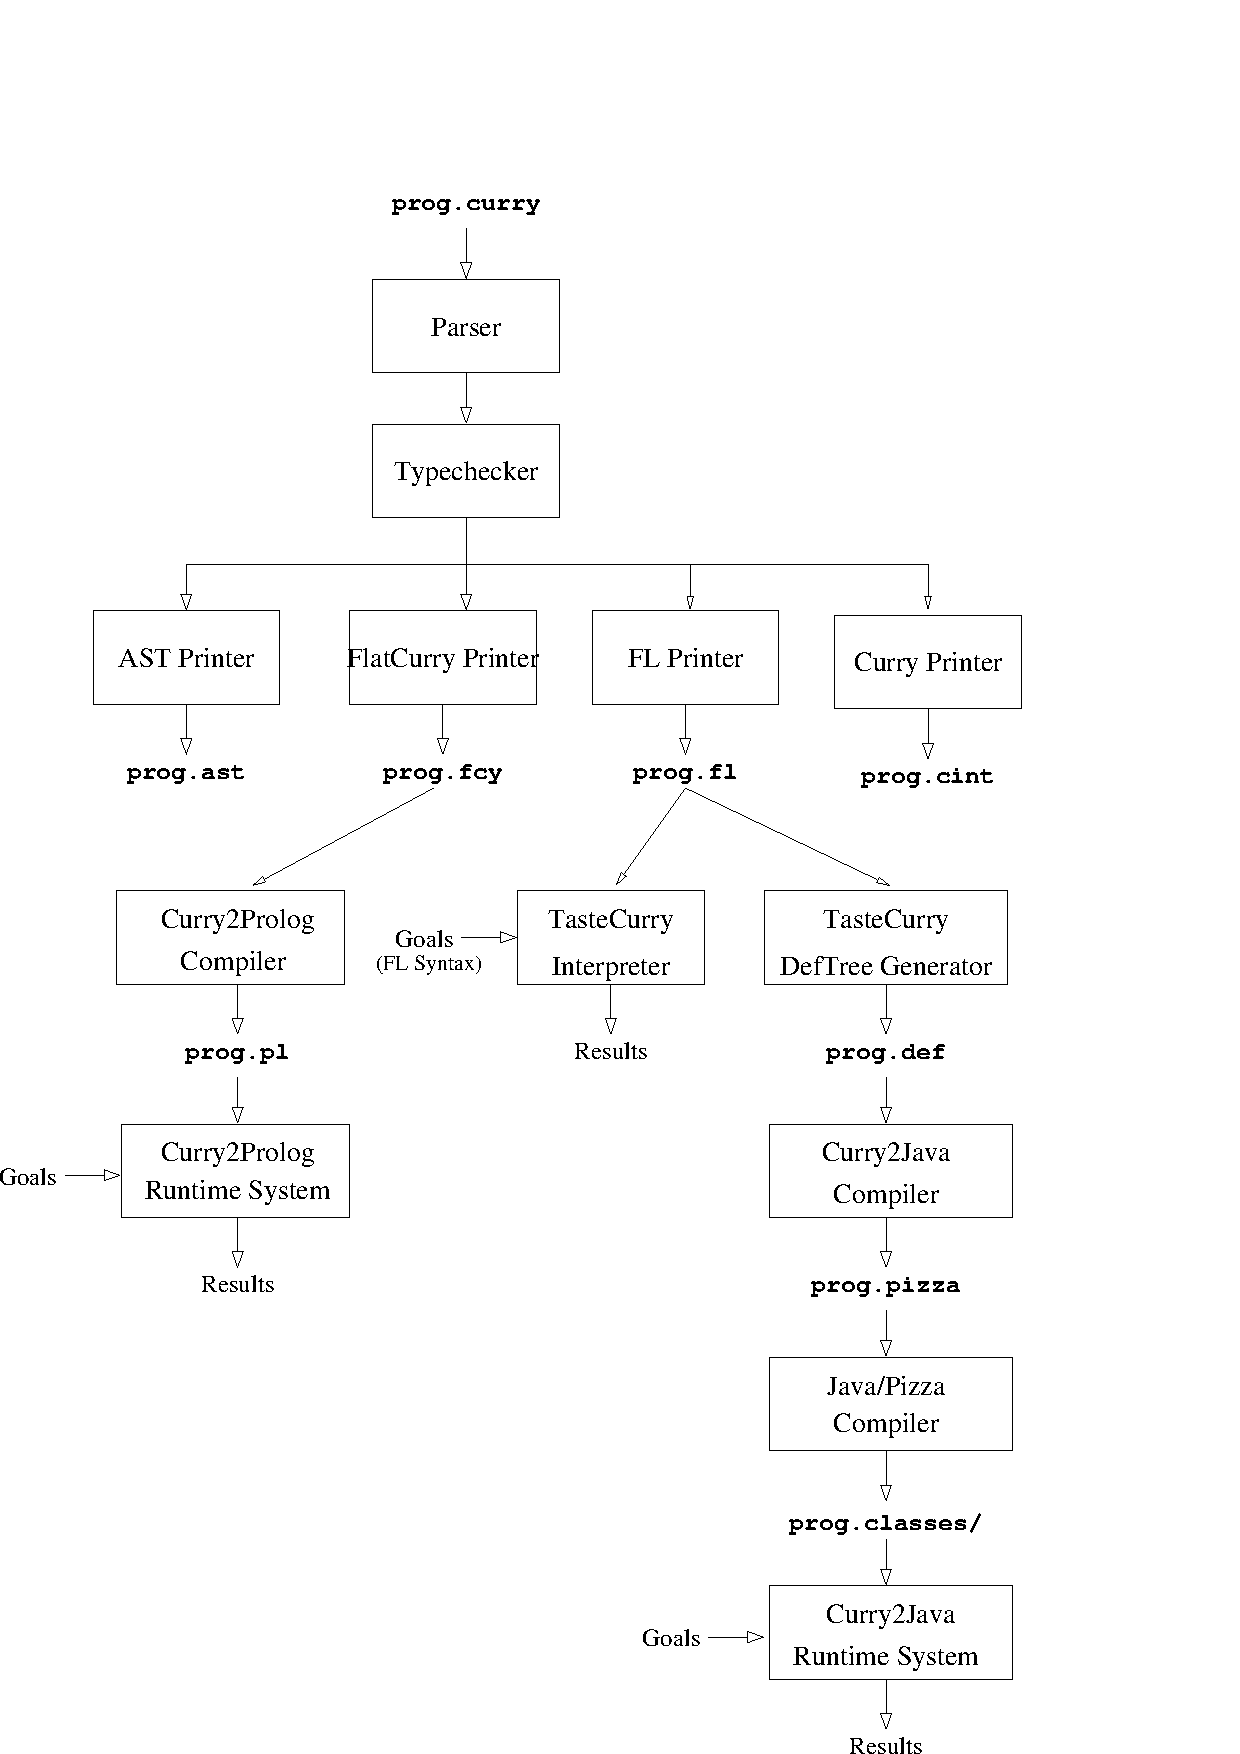
\includegraphics[scale=0.85]{pakcs_overview.jpg}
\end{center}\vspace{-5ex}
\caption{Overview of \CYS\label{fig-pakcs}}
\end{figure}

\section{Overview of the \CYS Distribution}

A schematic overview of the various components contained in
the distribution of \CYS and the
translation process of programs inside \CYS is shown in
Figure~\ref{fig-pakcs} on page~\pageref{fig-pakcs}.
In this figure, boxes denote different components of \CYS
and names in boldface denote files containing
various intermediate representations during the translation
process (see Section~\ref{sec-auxfiles} below).
The \CYS distribution contains a front end for reading (parsing and
type checking) Curry programs that can be also used by
other Curry implementations.
The back end (formerly known as ``Curry2Prolog''\index{Curry2Prolog})
compiles Curry programs into Prolog programs.
It also supports packages with constraint solvers for
arithmetic constraints over real numbers and finite domain constraints,
and further libraries for GUI programming, meta-programming etc.
It does not implement encapsulated search in full generality
(only a strict version of \code{findall} is supported
by the library \code{Control.Findall} which is part of the package
\code{searchtree}),
and concurrent threads are not executed in a fair manner.


%%% Local Variables: 
%%% mode: latex
%%% TeX-master: "manual"
%%% End: 

\section{Auxiliary Files}
\label{sec-auxfiles}

During the translation and execution of a Curry program with \CYS,
various intermediate representations of the source program are created
and stored in different files which are shortly explained in this section.
If you use \CYS, it is not necessary to know about
these auxiliary files because they are automatically generated
and updated. You should only remember the command for deleting
all auxiliary files (\ccode{cleancurry}, see Section~\ref{sec-general})
to clean up your directories.

Usually, the auxiliary files are invisible:
if the Curry module $M$ is stored in directory $dir$,
the corresponding auxiliary files are stored in directory
\ccode{$dir$/.curry/pakcs-$v$} where $v$ is the version of \CYS.
Thus, the auxiliary files produced by different versions of \CYS
causes no conflicts.
This scheme is also used for hierarchical module names:
if the module $D1.D2.M$ is stored in directory $dir$
(i.e., the module is actually stored in $dir/D1/D2/M.curry$),
then the corresponding Prolog program is stored in directory
\ccode{$dir$/.curry/pakcs-$v$/D1/D2}.

\medskip

The various components of \CYS create the following auxiliary files.
\begin{description}
\item[\code{prog.fcy}:] This file contains the Curry program
in the so-called ``FlatCurry'' representation where all functions are global
(i.e., lambda lifting has been performed) and pattern matching
is translated into explicit case/or expressions
(compare Appendix~\ref{sec-flatcurry}).
This representation might be useful for other back ends and
compilers for Curry and is the basis doing meta-programming in Curry.
This file is implicitly
generated when a program is compiled with \CYS.
It can be also explicitly generated by the
front end of \CYS:\pindex{pakcs frontend}
\begin{curry}
pakcs frontend --flat -i$\cyshome$/lib prog
\end{curry}
The FlatCurry representation of a Curry program is usually
generated by the front-end after parsing, type checking and eliminating
local declarations.

\item[\code{prog.fint}:] This file contains the interface
of the program in the so-called ``FlatCurry'' representation,
i.e., it is similar to \code{prog.fcy} but contains only exported
entities and the bodies of all functions omitted (i.e., ``external'').
This representation is useful for providing a fast access
to module interfaces.
This file is implicitly generated when a program is compiled with \CYS
and stored in the same directory as \code{prog.fcy}.

\item[\code{prog.icurry}:] This file contains the interface
of the program used by the front end for modular compilation.

\item[\code{prog.pl}:] This file contains a Prolog program
as the result of translating the Curry program with \CYS.

\item[\code{prog.po}:] This file contains the Prolog program
\code{prog.pl} in an intermediate format for faster loading
with SICStus-Prolog.

\item[\code{prog}:] This file contains the executable
after compiling and saving a program with \CYS
(see Section~\ref{sec:pakcs-commands}).
In contrast to the auxuiliary files, it is stored
in the main directory.

\end{description}


%%% Local Variables: 
%%% mode: latex
%%% TeX-master: "manual"
%%% End: 

\section{External Operations}
\label{sec-external-operations}

\index{function!external}\index{operation!external}\index{external operation}
An \emph{external operation} is an operation which have no defined rules
in a Curry program.
Instead, such an operation must be declared as \code{external}
in the Curry source code
and an implementation for this external operation
must be inserted in the corresponding back end.
In this section we describe how external operations
can be implemented in \CYS.

In general, an external operation is defined as follows
in the Curry source code:
\begin{enumerate}
\item
Provide a type declaration for the external operation somewhere
in the body of the appropriate Curry file.
Note that external operations should not be overloaded,
i.e., the type declaration should not contain any type class constraint.
\item
For external operations it is not allowed to define any
rule since their semantics is determined by an external implementation.
Instead of the defining rules, one has to write
\begin{curry}
f external
\end{curry}
somewhere in the file containing the type declaration for 
the external operation \code{f}.
\end{enumerate}
For instance, the addition on integers can be declared as
an external operation as follows:
\begin{curry}
(+) :: Int -> Int -> Int
(+) external
\end{curry}
Since \CYS compiles Curry programs into Prolog programs,
the actual implementation of an external operation
must be contained in some Prolog code that
is added to the compiled code by \CYS.
This can be done as follows:
%
\begin{enumerate}
\item
The Prolog code implementing the external operations declared
in module \code{M} must be put into the Prolog file \code{M.pakcs.pl}.
This file must be stored in the directory
containing the source code of the corresponding Curry module.
The contents of this file will be automatically added to the
compiler Curry program.

\item
In the general case (see below for exceptions),
the \CYS compiler generates a \emph{standard interface} to
external operations so that an $n$-ary operation is
implemented by an $(n+1)$-ary predicate where the last argument must
be instantiated to the result of evaluating the operation.
If \code{M.f} is the qualified name of the
external operation \code{f} defined in module \code{M},
then the predicate implementing this operation
must have the name \code{'M.f'} (note that this name
must be enclosed in ticks in Prolog).
The standard interface passes all arguments in their current form
to the predicate, i.e., it can be used if it is ensured that
all arguments are fully evaluated.
For the operation \code{(+)} shown above, this might not be the
case: in a call like \ccode{fac 4 + 3 * 7}, both arguments
mube be evaluated to some number before the external code
for the addition is called.
This can be ensured by enforcing the evaluation of the arguments
before calling the actual external operation.
For instance, the external operation for adding two integers
requires that both arguments must be evaluated to
a non-variable head normal form
(which is identical to the ground constructor normal form). Therefore,
the operation \ccode{+} can be implemented in the prelude by
\begin{curry}
(+)   :: Int -> Int -> Int
x + y = (prim_plusInt $\$$# y) $\$$# x

prim_plusInt :: Int -> Int -> Int
prim_plusInt external
\end{curry}
where \code{prim_plusInt} is the actual external operation implementing
the addition on integers.
Hence, the Prolog code implementing \code{prim_plusInt} can be as
follows (note that the arguments of \code{(+)} are passed in reverse
order to \code{prim_plusInt} in order to ensure a left-to-right
evaluation of the original arguments by the calls to \code{(\$\#)}):
\begin{curry}
'Prelude.prim_plusInt'(Y,X,R) :- R is X+Y.
\end{curry}

\item
The \emph{standard interface for I/O actions}, i.e., external operations
with result type \code{IO~a}, assumes that the I/O action
is implemented as a predicate (with a possible side effect)
that instantiates the last argument to the returned value of type \ccode{a}.
For instance, the primitive predicate \code{prim_getChar}
implementing the prelude I/O action \code{getChar}
can be implemented by the Prolog code
\begin{curry}
'Prelude.getChar'(C) :- get_code(N), char_int(C,N).
\end{curry}
where \code{char_int} is a predicate (from the \CYS run-time system)
relating the internal Curry representation of a character
with its ASCII value.

\item
If some arguments passed to the external operations are not fully evaluated
or the external operation might suspend, the implementation must follow
the structure of the \CYS run-time system by using the \emph{raw interface}
instead of the standard interface.
For this purpose, it is necessary to tell \CYS about the
non-standard interface.
Thus, if the Curry module \code{Mod} contains external operations
where the standard interface should not be used,
there must be a file named \code{Mod.pakcs} containing the
specification of these external operations. The contents of this file
is in XML format and has the following general structure:\footnote{%
\url{http://www.informatik.uni-kiel.de/~pakcs/primitives.dtd} contains a DTD
describing the exact structure of these files.}
\begin{curry}
<primitives>
  $\textit{specification of external operation~}f_1$
  $\ldots$
  $\textit{specification of external operation~}f_n$
</primitives>
\end{curry}
The specification of an external operation $f$
with arity $n$ has the form
\begin{curry}
<primitive name="$f$" arity="$n$">
  <entry>pred[raw]</entry>
</primitive>
\end{curry}
where \code{pred} is the name of a predicate
implementing this operation. Note that the operation $f$ must be
declared in module \code{Mod}: either as an external operation
or defined in Curry by equations. In the latter case,
the Curry definition is not translated but calls to this operation
are redirected to the Prolog code specified above.

Furthermore, the list of specifications can also contain entries of the form
\begin{curry}
<ignore name="$f$" arity="$n$" />
\end{curry}
for operations $f$ with arity $n$ that are declared in module \code{Mod}
but should be ignored for code generation, e.g., since they are
never called w.r.t.\ to the current implementation of external operations.
For instance, this is useful when operations that can
be defined in Curry should be (usually more efficiently) are implemented
as external operations.

The suffix \ccode{[raw]} used above indicates that the corresponding Prolog
code follows the structure of the \CYS compilation scheme.
For instance, if we want to use the raw interface for the external operation
\code{prim_plusInt},
the specification file \code{Prelude.pakcs} must have an entry of the form
\begin{curry}
<primitive name="prim_plusInt" arity="2">
  <entry>prim_plusInt[raw]</entry>
</primitive>
\end{curry}
In the raw interface, the actual implementation of
an $n$-ary external operation consists
of the definition of an $(n+3)$-ary predicate $pred$.
The first $n$ arguments are the corresponding actual arguments.
The $(n+1)$-th argument is a free variable which must be
instantiated to the result of the operation call after
successful execution. The last two arguments
control the suspension behavior of the operation
(see \cite{AntoyHanus00FROCOS} for more details):
The code for the predicate $pred$
should only be executed when the $(n+2)$-th argument
is not free, i.e., this predicate has always the
SICStus-Prolog block declaration
\begin{curry}
?- block $pred$(?,$\ldots$,?,-,?).
\end{curry}
In addition, typical external operations should suspend
until the actual arguments are instantiated. This can be ensured
by a call to \code{ensureNotFree} or \code{(\$\#)}
before calling the external operation. Finally, the
last argument (which is a free variable at call time)
must be unified with the $(n+2)$-th argument
after the operation call is successfully evaluated
(and does not suspend). Additionally, the actual (evaluated) arguments
must be dereferenced before they are accessed.
Thus, an implementation
of the external operation for adding integers is as follows in the raw interface:
\begin{curry}
?- block prim_plusInt(?,?,?,-,?).
prim_plusInt(RY,RX,Result,E0,E) :-
     deref(RX,X), deref(RY,Y), Result is X+Y, E0=E.
\end{curry}
Here, \code{deref} is a predefined predicate for dereferencing the
actual argument into a constant (and \code{derefAll} for dereferencing
complex structures).
\end{enumerate}
%
Note that arbitrary operations implemented in C or Java can be connected to
\CYS by using the corresponding interfaces of the underlying Prolog system.


%%% Local Variables: 
%%% mode: latex
%%% TeX-master: "manual"
%%% End: 


% Index
\addcontentsline{toc}{section}{Index}
\printindex

\end{document}
